\chapter{Introduction}
\section{Abstract}
\label{sec:abstract}
Ever since Nvidia released their RTX GPU family, real time raytracing applications rapidly rose to popularity. To allow this, these GPUs feature hardware acceleration for ray traversal. However, acceleration structures are limited to single-level instancing and to a fixed function traversal behavior. This does not allow for techniques like dynamic level of detail that reduces CPU-GPU communication in between frames nor the use of multi-level-instancing to reduce scene size on the GPU.\\ Won-Jong et al. \cite{traversalArticle} proposed the insertion of programmable instances into acceleration structures. In this thesis we will use programmable instances to allow for Multi-Level-Instancing and dynamic Level-of-Detail by using the Vulkan Raytracing API. This will allow us to render the Moana Island production asset by Disney in real time while saving multiple GBs of VRAM.
\section{Preview}
\label{sec:preview}
During this thesis, a raytracing application is developed that is implementing the developed concept. The next two pages are some renders which were made with the definitive version of the application.
\newpage
\begin{figure}
    \centering
    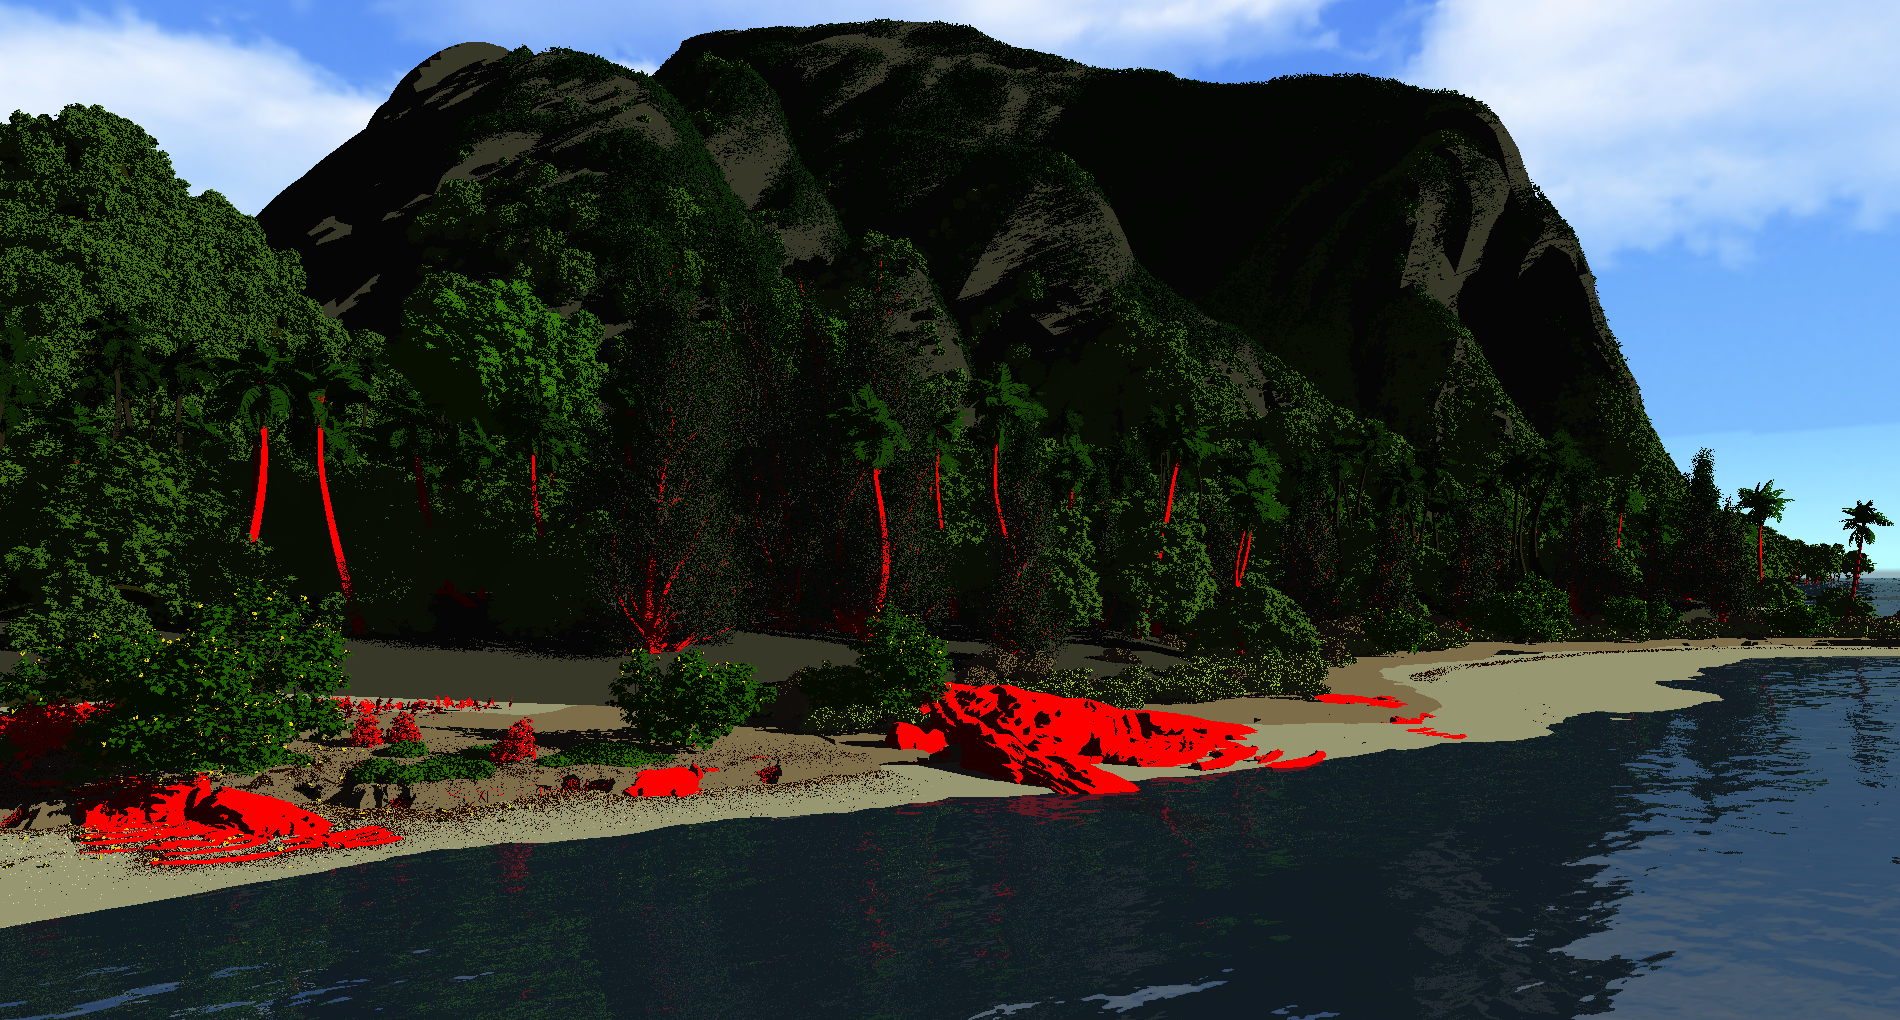
\includegraphics[width=.7\textwidth]{images/preview/Moana Overview.PNG}
    \caption{Overlook of Moana Island.}
    \label{fig:preview-pic3}
\end{figure}

\begin{figure}
    \centering
    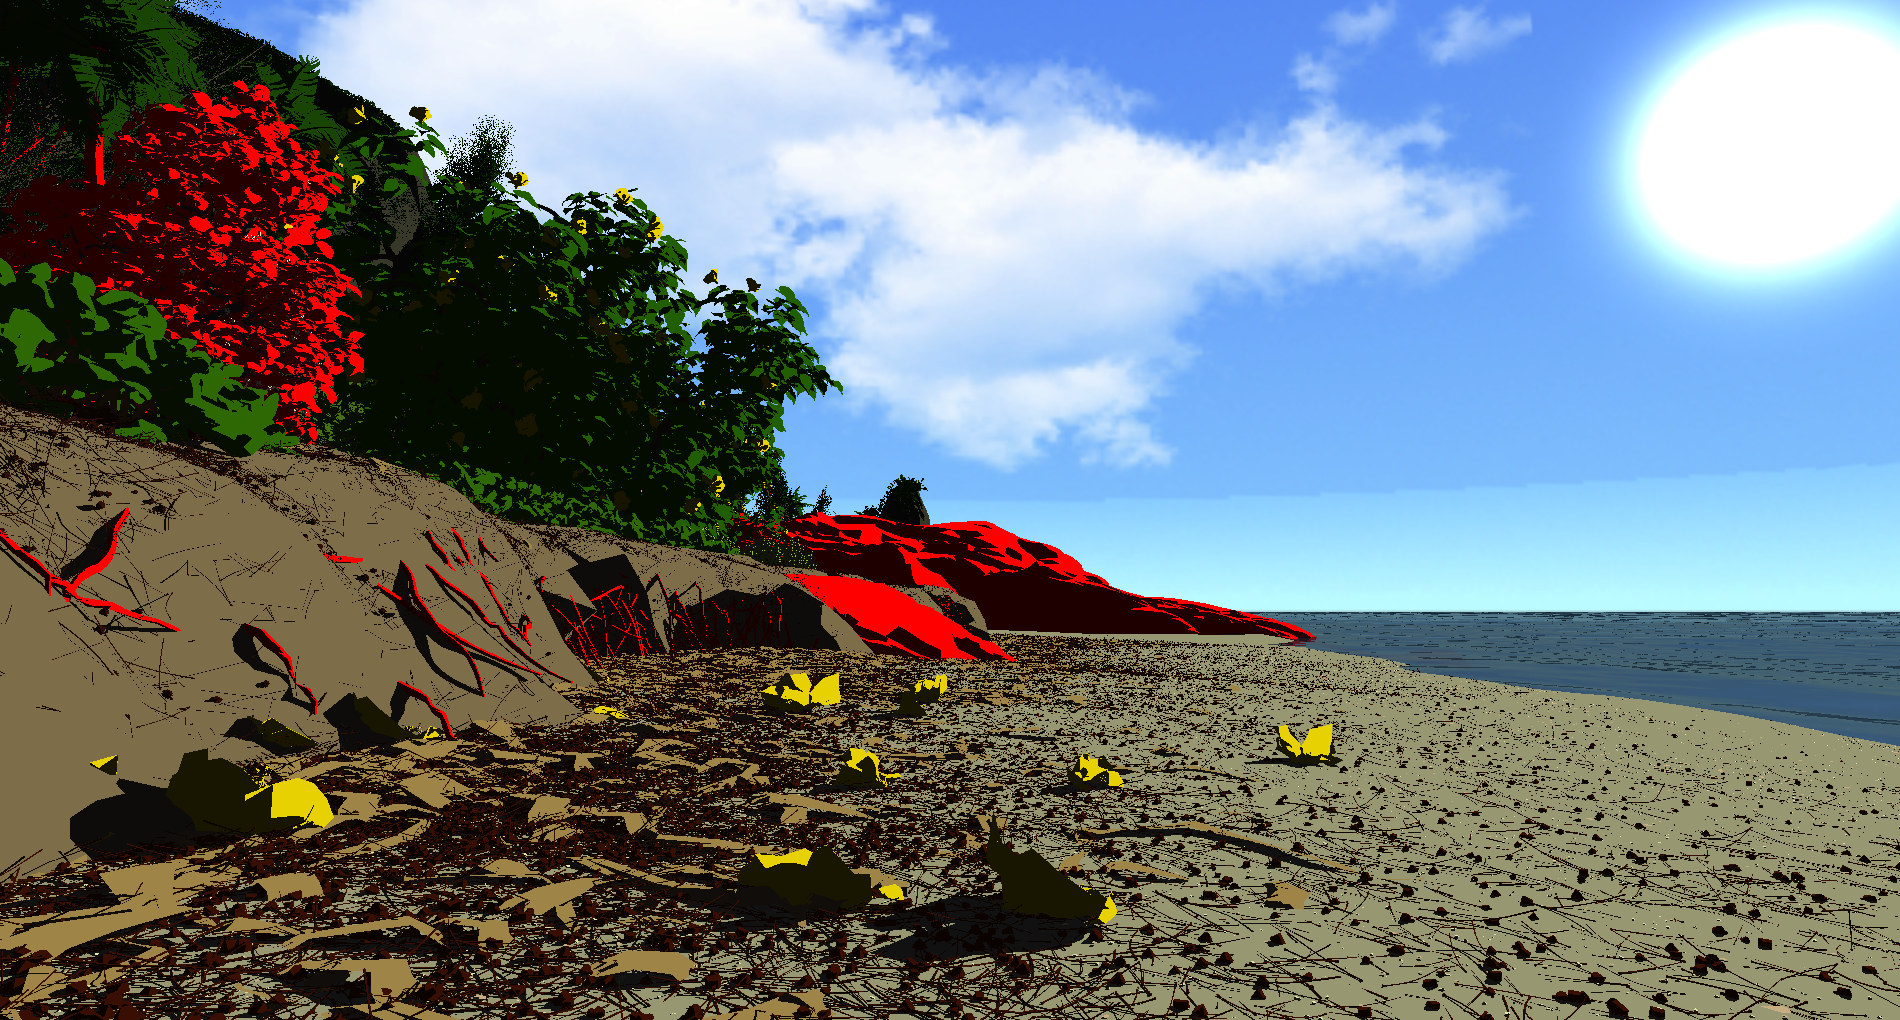
\includegraphics[width=.7\textwidth]{images/preview/Moana Beach.PNG}
    \caption{Moana Island uses millions of instances.}
    \label{fig:preview-pic4}
\end{figure}

\begin{figure}
    \centering
    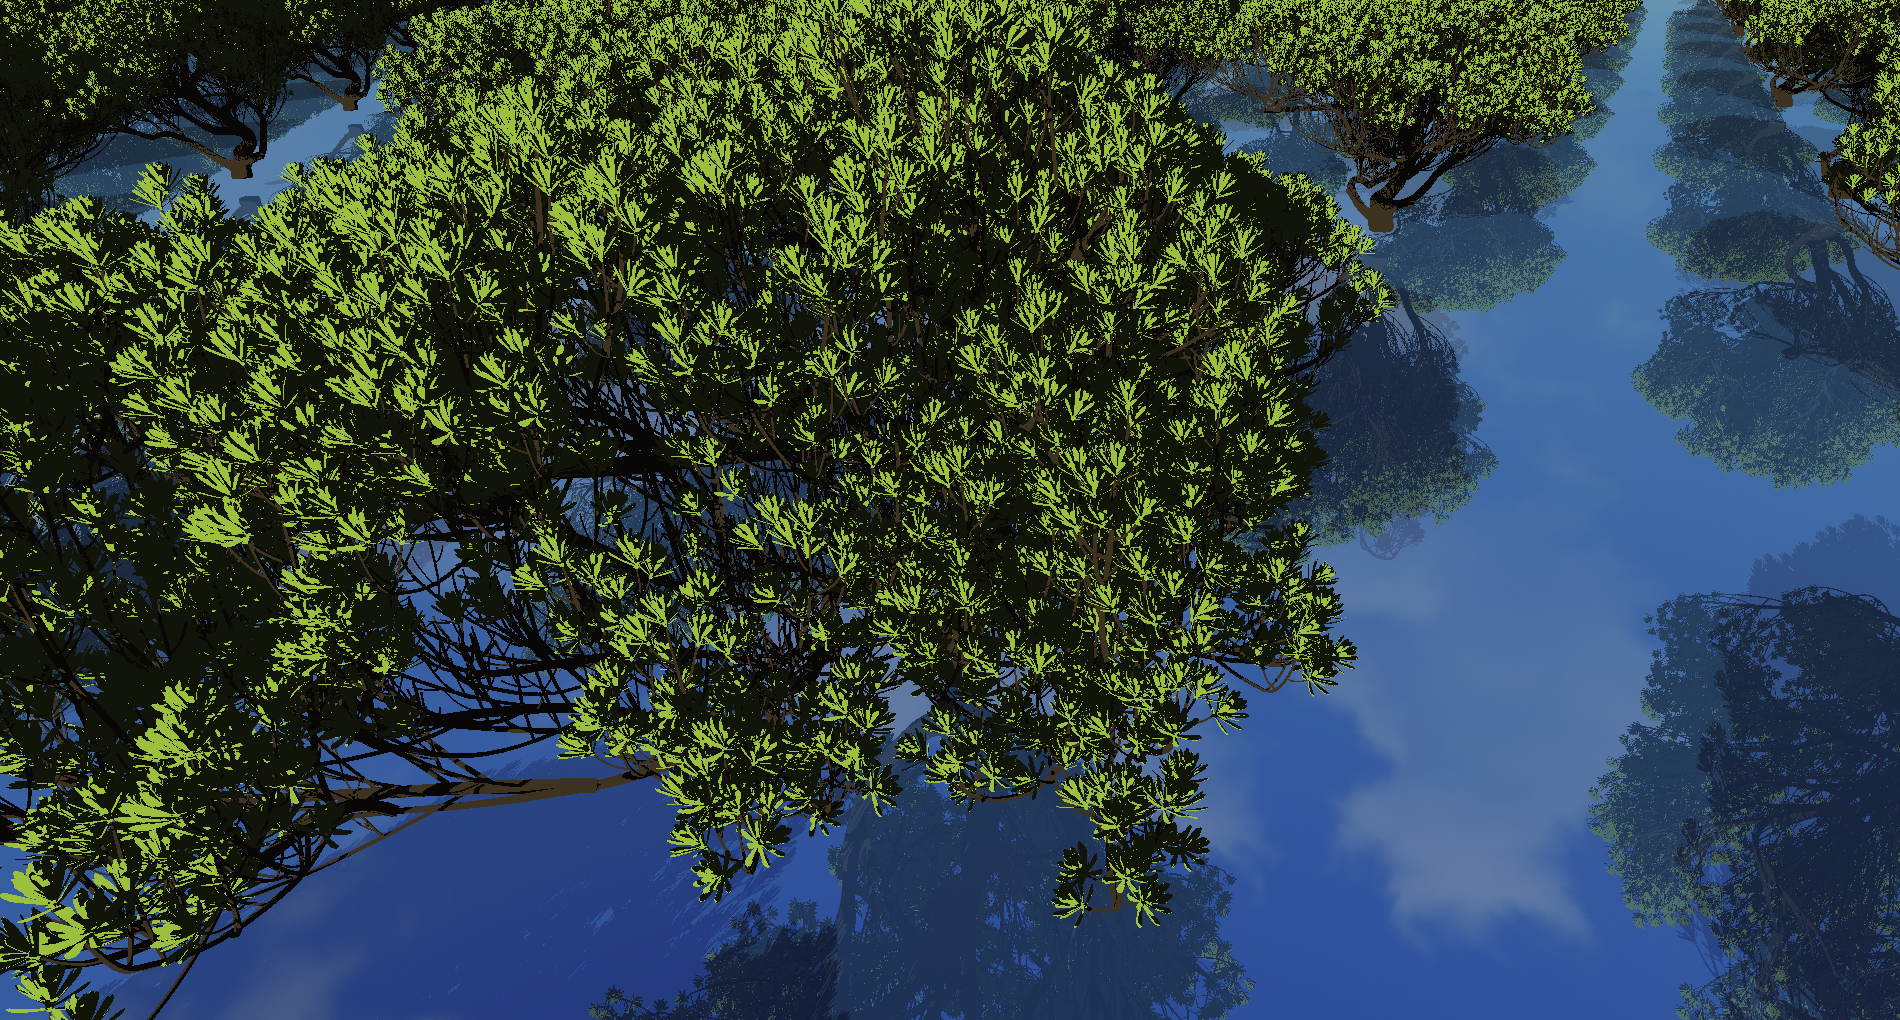
\includegraphics[width=.7\textwidth]{images/preview/Tree.PNG}
    \caption{A tree with instanced leaves in a forest of instanced trees.}
    \label{fig:preview-pic1}
\end{figure}

\begin{figure}
    \centering
    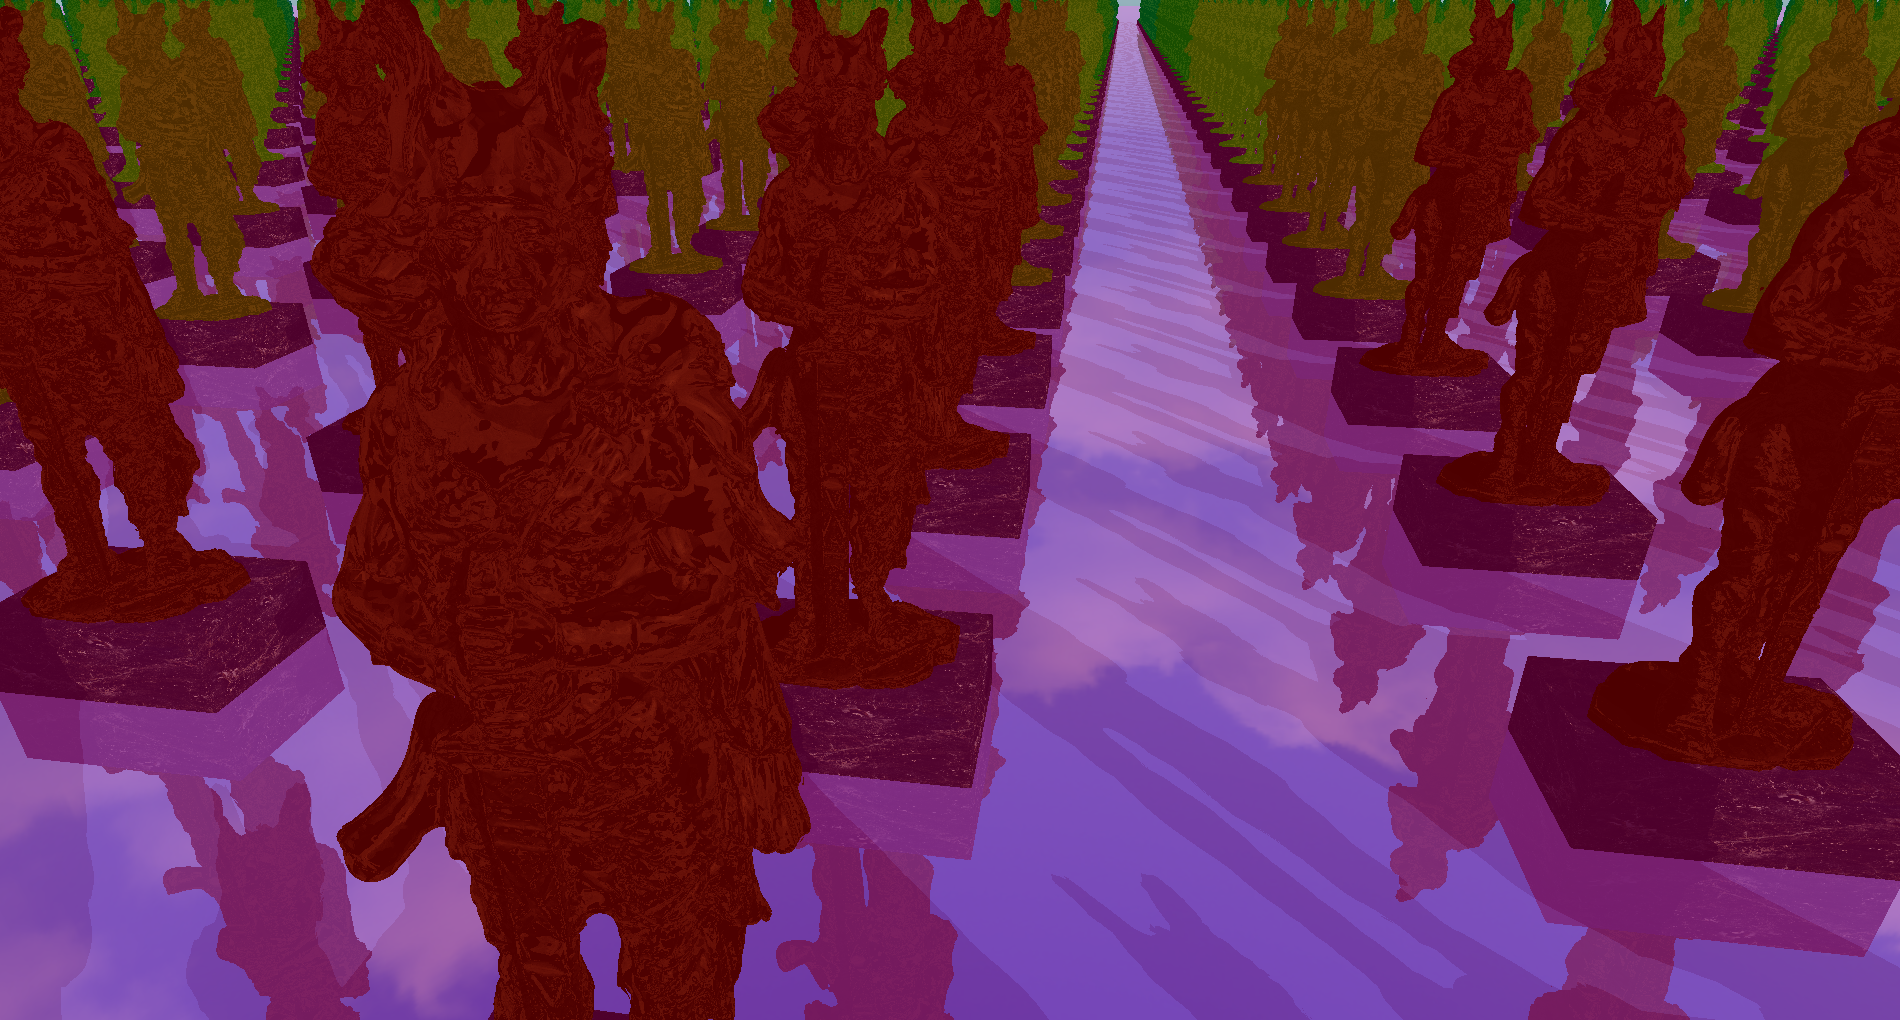
\includegraphics[width=.7\textwidth]{images/preview/LOD-Select.PNG}
    \caption{Dynamic selection for Level-of-Detail.Red:High,Green:Low.}
    \label{fig:preview-pic2}
\end{figure}

\begin{figure}
    \centering
    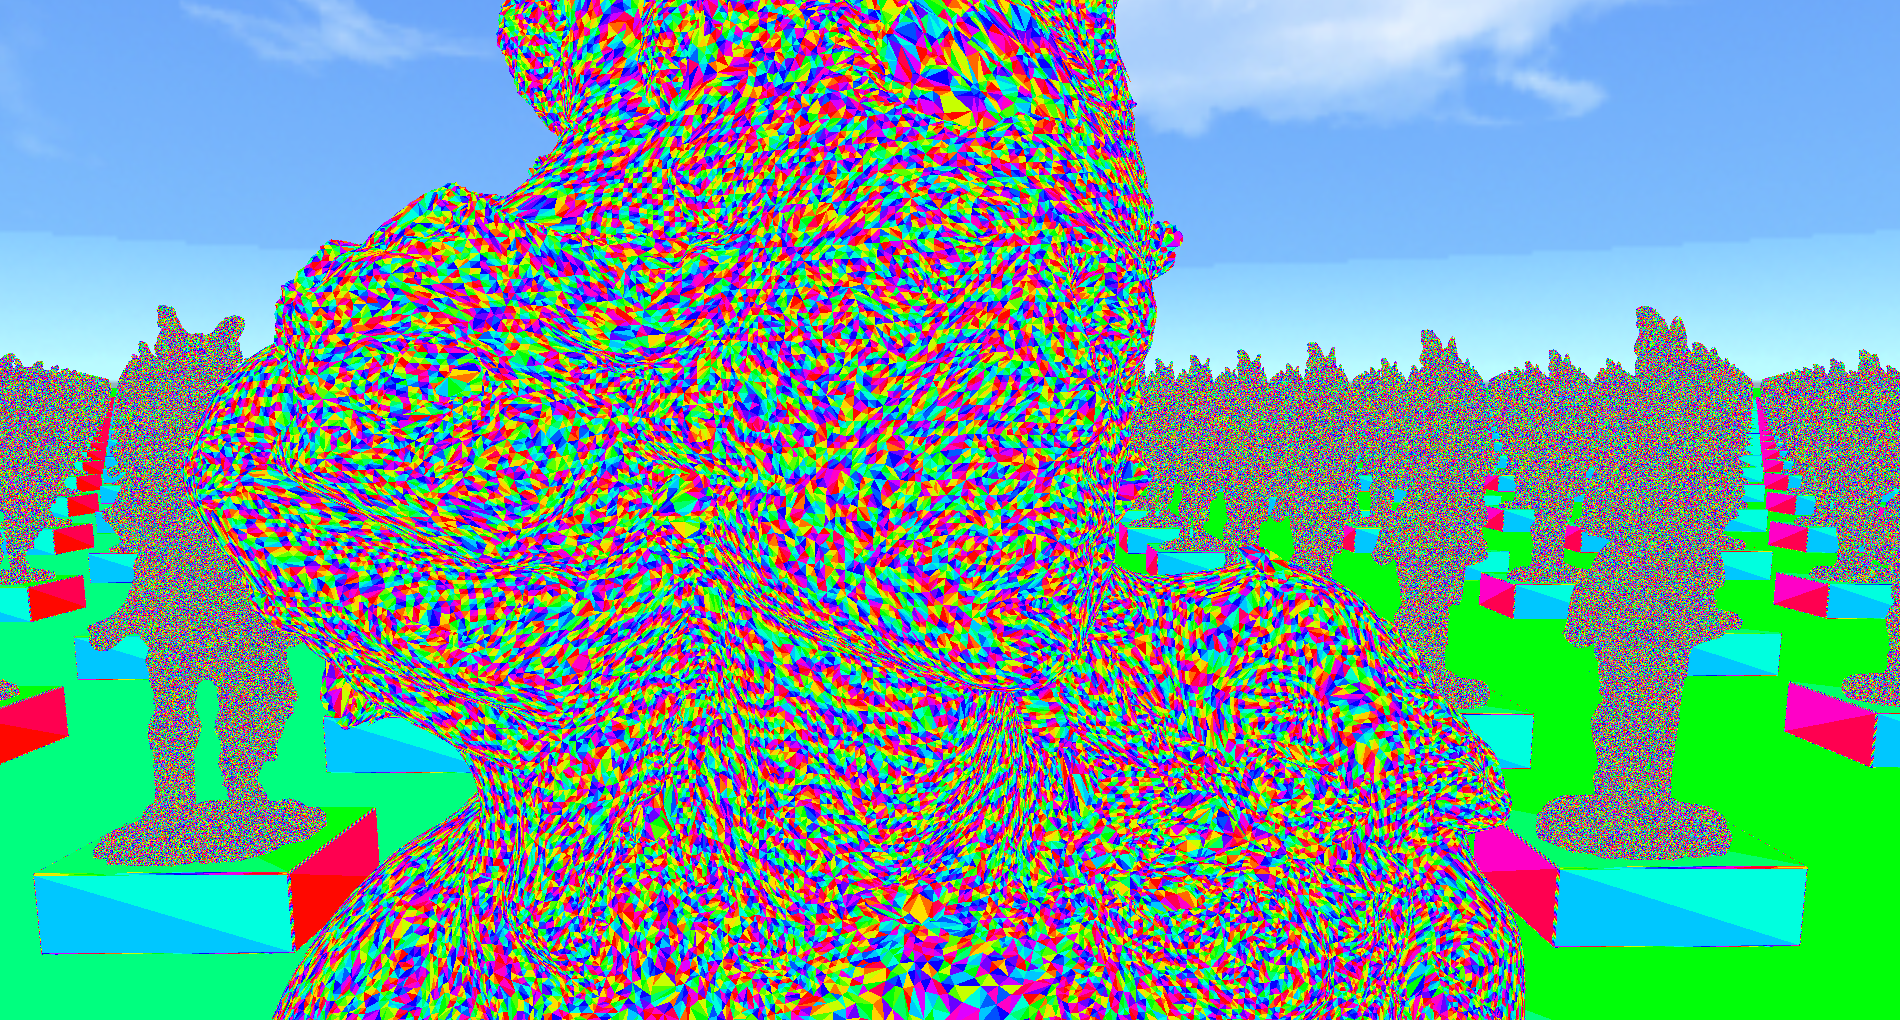
\includegraphics[width=.7\textwidth]{images/preview/LOD-Max.PNG}
    \caption{Mesh in its highest resolution.}
    \label{fig:preview-pic6}
\end{figure}

\begin{figure}
    \centering
    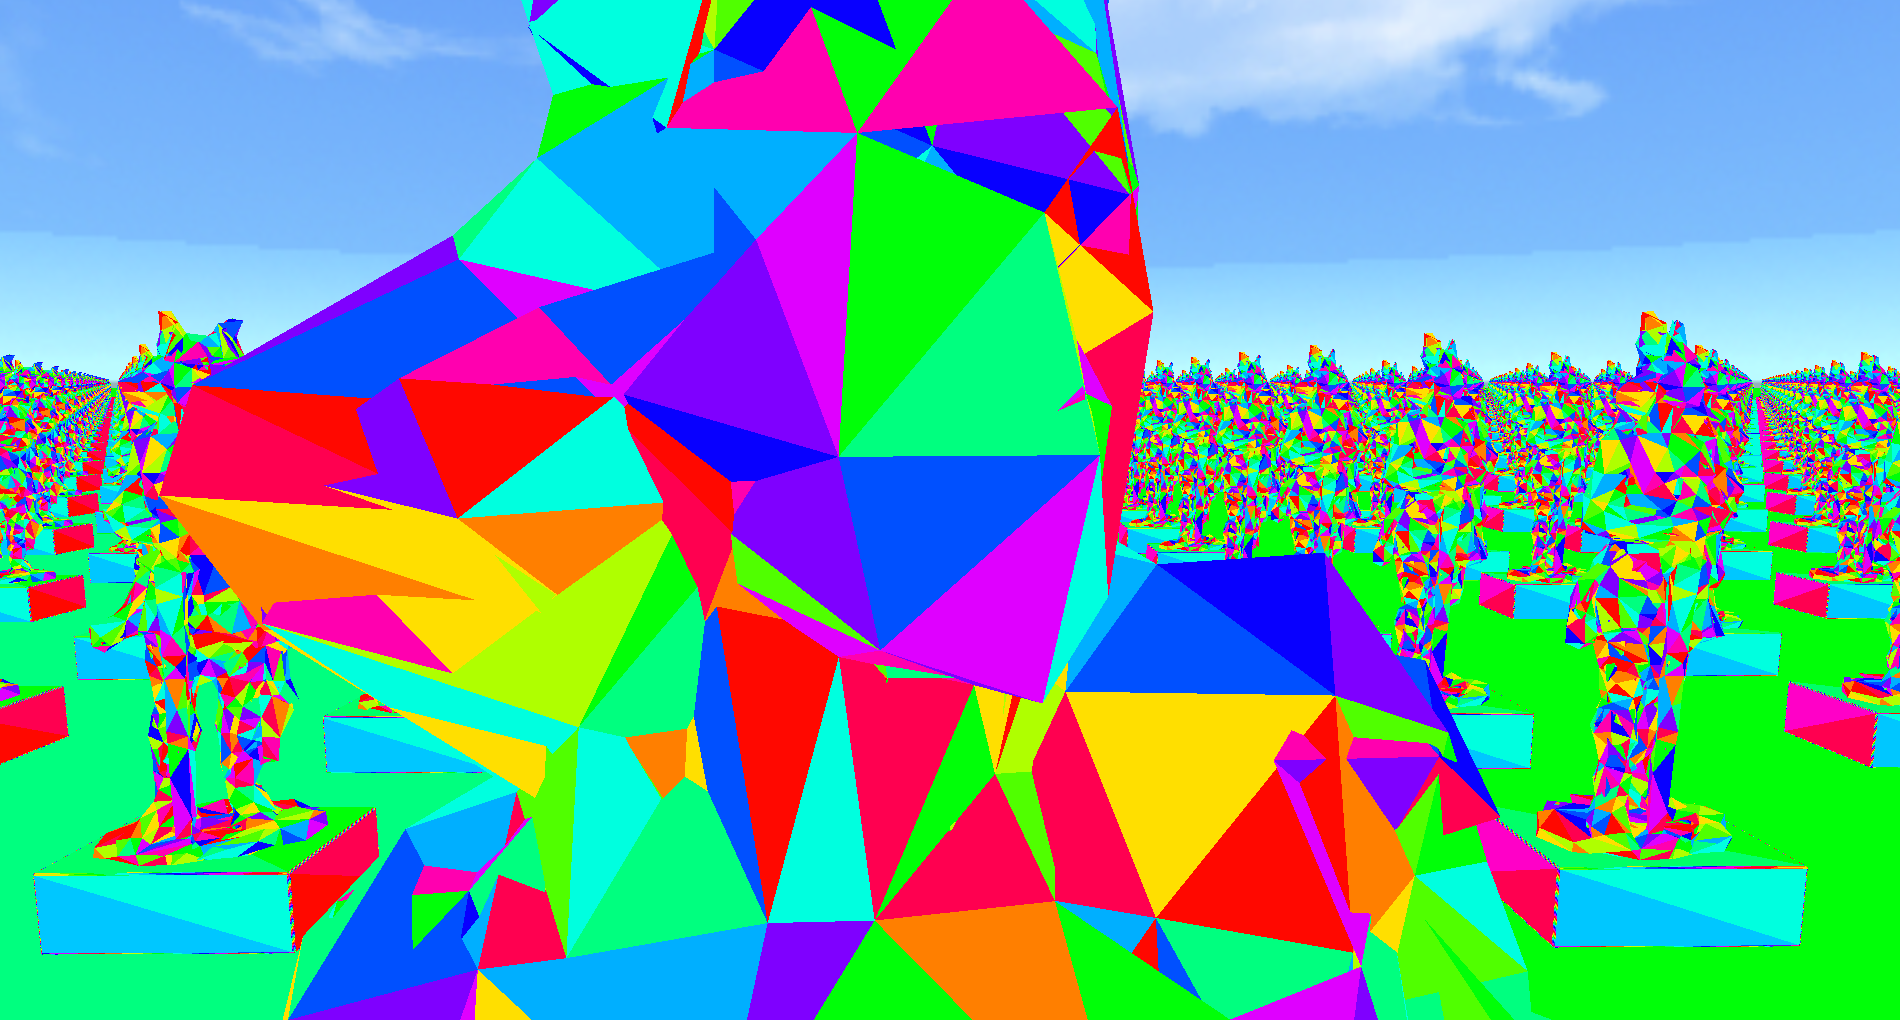
\includegraphics[width=.7\textwidth]{images/preview/LOD-Min.PNG}
    \caption{Mesh in its lowest resolution.}
    \label{fig:preview-pic8}
\end{figure}

\chapter{Basics}
To begin, we will cover basics of computer graphics. In this chapter we will introduce transformations, rasterization, raytracing, and acceleration structures. Later in this chapter we will look at the Vulkan API as well as scene graph processing. Inspiration for this section originates from the CG lecture at KIT. Relevant material is available in the PBRT book \cite{pbrBook} and the scratchapixel website \cite{scrathAPixel}.
\section{Transformations}
\label{sec:transformations}
Transformations are an integral part for any graphics application. Any vector can be rotated and scaled by applying a matrix transform ${T} \in \mathbb{R}^{3\times3}$ to it. This matrix commonly consists of an orthonormal rotation matrix ${R}$ and a diagonal scaling matrix ${S}$.\\
Given those two properties indicates that they are both invertible, which can be used to undo a transform. Using a ${3\times3}$ matrix however has the limitation that it is unable to represent vector translation since it is not a linear operation.\\
A common approach for representing translation using matrices are homogeneous coordinates. They extend the 3D translation into the fourth dimension.\\
Let $v$ be a position in 3D space, $d$ a direction vector, $n$ a normal vector on a surface, ${R}$, ${S}$ as above and $t$ a translation vector. Using homogeneous coordinates applies the three transformations on the three vectors in separate ways. The combined transform ${T}$ can be described as follows:\\
\[
{T} = 
\begin{pmatrix}
1 & 0 & 0 & t_1 \\
0 & 1 & 0 & t_2 \\
0 & 0 & 1 & t_3 \\
0 & 0 & 0 & 1
\end{pmatrix}
\begin{pmatrix}
 \mbox{\LARGE ${R}$} & \begin{matrix} 0 \\ 0 \\ 0\end{matrix} \\
 \begin{matrix} 0 & 0 & 0\end{matrix} & 1
\end{pmatrix}
\begin{pmatrix}
 \mbox{\LARGE ${S}$} & \begin{matrix} 0 \\ 0 \\ 0\end{matrix} \\
 \begin{matrix} 0 & 0 & 0\end{matrix} & 1
\end{pmatrix}
\]
Applying $T$ to a 3D Position:
\[
T
\begin{pmatrix}
 v_1\\
 v_2\\
 v_3\\
 1
\end{pmatrix}
=
\begin{pmatrix}
 v'_1\\
 v'_2\\
 v'_3\\
 1
\end{pmatrix}\]
\newpage
Because of the fourth element the vector is translated by $t$. This is not the case for direction vectors, where a translation is undesired. In short, the homogeneous vector for $d$ needs to have zero as its fourth element.
\[
T
\begin{pmatrix}
 d_1\\
 d_2\\
 d_3\\
 0
\end{pmatrix}
=
\begin{pmatrix}
 d'_1\\
 d'_2\\
 d'_3\\
 0
\end{pmatrix}\]
This results in $d$ being only rotated and scaled by $R$ and $S$ with the translation ignored.\\
Vector transformations are also used for surface normals, which do not behave like positions or directions. Transforming these requires the transposed inverse of the transformation. I will give no prove for this. One can be found on the scratchapixel \cite{scrathAPixel} website. The transformation of a surface normal is shown below.
\[
(T^{-1})^\intercal
\begin{pmatrix}
 n_1\\
 n_2\\
 n_3\\
 0
\end{pmatrix}
=
\begin{pmatrix}
 n'_1\\
 n'_2\\
 n'_3\\
 0
\end{pmatrix}\]
Any transformation matrix $T$ can be seen as a switch in coordinate systems. For better understanding, any transform matrix that will be used from now on will, in most cases, be named as fromToTarget(-Transform) or an equivalent name.\\
Using different coordinate systems is essential for computer graphics as it allows for transforming any object space mesh into world space and into view space. This can go even further and can transform view space objects into a 2D projection with the third coordinate indicating the distance from the 2D projection plane.\\
Homogeneous matrices are quite flexible and for most purposes sufficient to be used in 3D rendering applications, as they describe coordinate system switches, projections, translation, rotation, scaling and even sheering.
\section{Raytracing and Rasterization} 
The two pillars of computer graphics are Rasterization and Raytracing. Both are techniques for image rendering from 3D scenes. However, those two follow drastically different approaches.\\
\subsection{Rasterization}
\label{sec:rasterization}
Rasterization is a rendering processes that projects triangles through a number of transforms onto an image. Its input are triangles in a given coordinate system. They are then transformed though a model-view-projection-matrix into projection space in which the viewable space is a unit cube $[-1,1]^3$. Following this step, any triangles outside of this cube are clipped. Clipping is a way of cutting off parts of a triangle in such a way that only its contents that are inside of the unit cube remain. As the next step, the triangles are rasterized. This can be seen as a kind of drawing process that creates fragments for each pixel that the triangle occupies when it is projected onto the image. For each of these fragments their color can then be computed. Lastly fragments which belong to the same pixel are blended together following a bunch of tests that determine the final color. An example for the projection of triangles can be seen in figure \ref{fig:cgRasterization}.
\begin{figure}
    \centering
    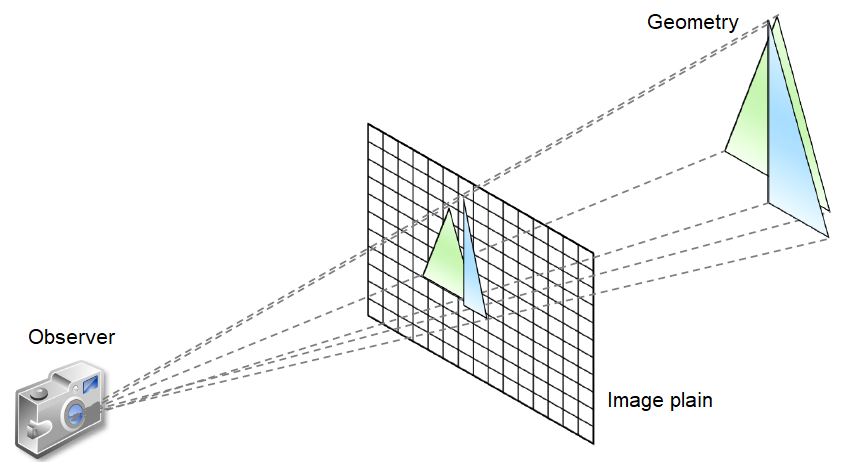
\includegraphics[width=0.9\textwidth]{images/showcase/CgRasterization.PNG}
    \caption{Projection of triangles onto the screen using rasterization. Source:CgLecture@KIT.}
    \label{fig:cgRasterization}
\end{figure}
Rasterization is the industry standard of rendering in real time applications, since each triangle computation is almost independent from each other. In addition to this, rasterizing a triangle onto screenspace is very efficient. A normal GPU can easily throughput a few hundred million triangles every frame. However, rasterization is primarily a projection onto the screen. Selecting the nearest primitive for each pixel means that this approach is lighting independent. This makes calculating shadows quite troublesome and prune to artifacts. Common lighting techniques are for example shadow mapping \cite{computergraphicsAndImageProcessing}.\\
As stated, the biggest advantage is streamlining, given the fact that GPUs are designed with optimizing rasterization as well as it being researched and used to a high degree. However, calculating shadows and more advanced lighting effects does pose quite the challenge to implement. That applications prefer rasterization stems mostly from the history behind the process, as hardware simply was not performant enough to do raytracing on a large scale as real time applications would require.
\subsection{Raytracing}
Raytracing follows a different approach. Instead of projecting triangles onto screen space, it instead tries to model the way light travels around the scene. For every pixel, a primary ray is cast into the scene and the first object it intersects is computed. Using this intersection point, the pixel color is calculated by casting shadow, reflection, and transmission rays into the scene and reading in the triangles texture by mapping the triangle onto a 2D texture. This procedure is called UV-mapping. A visualization can be seen in figure \ref{fig:cgRayTrace}.\\
Raytracing is inherently parallel, which is optimal for GPU computation. However, there are drawbacks when it comes to performance. Tracing a ray for every pixel and then alone compute the first intersected primitive takes $O(w\cdot h\cdot log(n))$ and that is with using an acceleration structure. With $w$ and $h$ being the windows width/height and $n$ being the number of triangles inside of the scene. Acceleration structures can be used to speed up the process of finding an intersection for a ray and allow for $O(log(n))$ for finding an intersection. However, this number is only for using primary rays. The amount of rays can grow exponentially as soon as reflections and transmissions become involved. For the longest time this was unsuitable for most GPUs. These days however and for non-real-time purposes, raytracing is a viable option. This can be used to simulate lighting quite accurately.\\
Now more applications are starting to use raytracing even in the real-time apartment, as GPU retailers (mostly Nvidia) are starting to support more and more raytracing functionality in their drivers and hardware. This goes as far as dedicated raytracing cores whose sole purpose is to traverse acceleration structures as efficiently as possible, which makes even real-time raytracing possible.
\label{sec:raytracing}
\begin{figure}
    \centering
    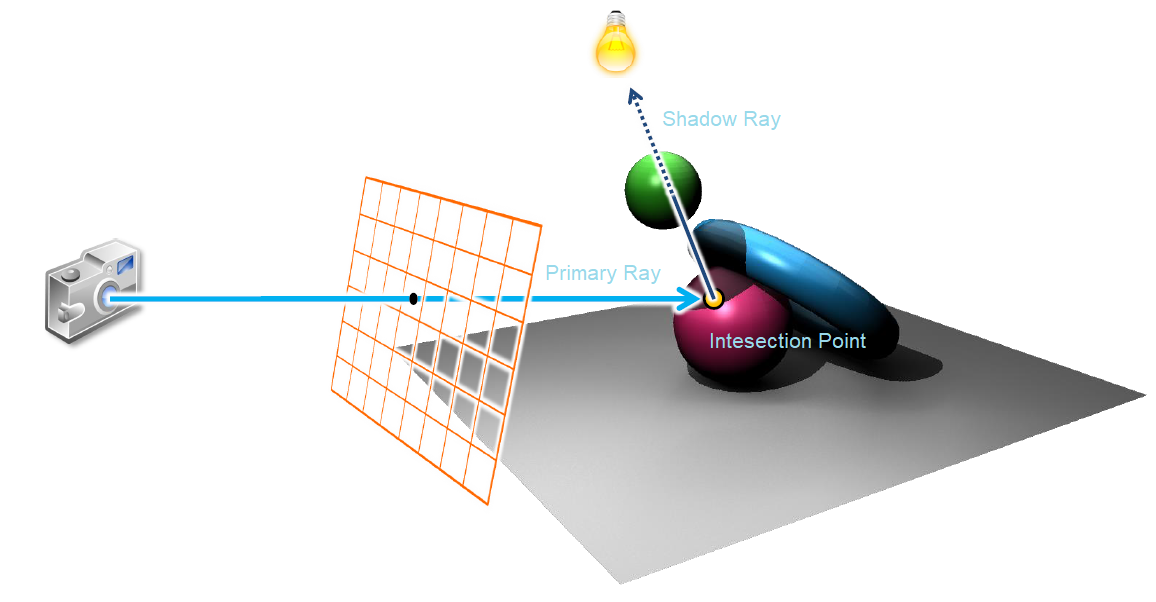
\includegraphics[width=.9\textwidth]{images/showcase/cgRayTracingImg.PNG}
    \caption{Ray Tracing with primary and shadow ray. Source CgLecture@KIT.}
    \label{fig:cgRayTrace}
\end{figure}

\subsection{Usage}
\label{sec:RayRasterUsage}
The decision which technique to use is dependent on purpose. For high framerate renders, that can live with cutting on some realism, rasterization is the go-to option. However, for any non-real-time purposes and, with sufficient processing power even real time applications, raytracing is certainly an option.\\
A common technique right now uses a combination of the two. Casting primary rays is quite expensive, so the visibility technique firstly computes the visible triangles on the screen using rasterization. It might also be used to calculate the shadows using shadow mapping. Raytracing then deals with reflections and transparency.\\
For the application and testing environment that is developed alongside this thesis, I will use only raytracing to assess  the limits of what it can currently do.
\cite{rayRasterNvidiaBlog}
\section{Acceleration Structures}
Raytracing suffers from a high computational requirement to find ray intersections. To speed up the process of intersection computation acceleration structures are used to prevent many unnecessary intersection tests. Typically, they speed up intersection computation from $O(n)$ to $O(log(n))$. Logarithmic growth leads to good traversal speed even for large scenes, as a factor increase in size only represents a constant increase in operations.
In general acceleration structures can be divided into tree-based and grid-based. I will introduce one example of each, the difference being whether it divides either space or primitives in its sub-trees.
\begin{figure}
    \centering
    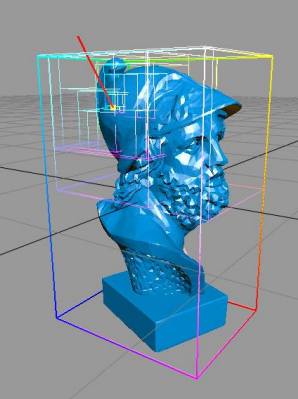
\includegraphics[width=.5\textwidth]{images/showcase/CgLectureBVH.PNG}
    \caption{A BVH for a triangle mesh. Source:CgLecture@KIT.}
    \label{fig:cgBVH}
\end{figure}
\newpage
\subsection{BVHs}
\label{sec:BVH}
A BVH, short for Bounding-Volume-Hierarchy, represents a tree-based layout in which the primitives are contained in bounding volumes, most commonly Axis-Aligned-Bounding-Boxes (AABBs). These in turn are then grouped into other AABBs. The result is a tree of bounding boxes with a height of $O(log(n))$. The most common construction process recursively partitioning primitives. When constructing AABBs for a number of primitives the process normally starts with splitting the primitives for each node in half along a cutting line, for example the axis of the largest extent. Then the primitives are sorted along that axis and inserted either into the right or left sub-tree. This is done is such a way that there are approximately an equal number of primitives on each side. If this is the case the tree can be called balanced. Construction resumes for the sub-trees, until only a predefined number of primitives are left per AABB. These are the leaves of the tree. Figure \ref{fig:cgBVH} shows the intersected AABBs by a ray.
Dividing primitives does not only work for triangles but for all kinds of geometry. In this case smaller AABBs which represent another already constructed BVH. These BVHs are reused multiple times and are instanced with different transformations. In this thesis, there will be occurrences where splitting geometry for a BVH is a requirement. This is the case when the number of geometry is more than the maximum allowed by the driver(Our case: $2^{24}$). Sorting such a large number of instances is inefficient (O(n log(n)). So, a way to split them is along the axis of largest extent. Then the median of all AABBs along this axis is computed. With this median the AABBs are then split into either the left or the right sub-tree depending on which side they are on. When using a median, the split is not 50/50, but still good enough, so that the resulting tree remains balanced. The median works best if the geometry is evenly distributed.\\
\begin{figure}
\subfigure[Overlapping AABBs]{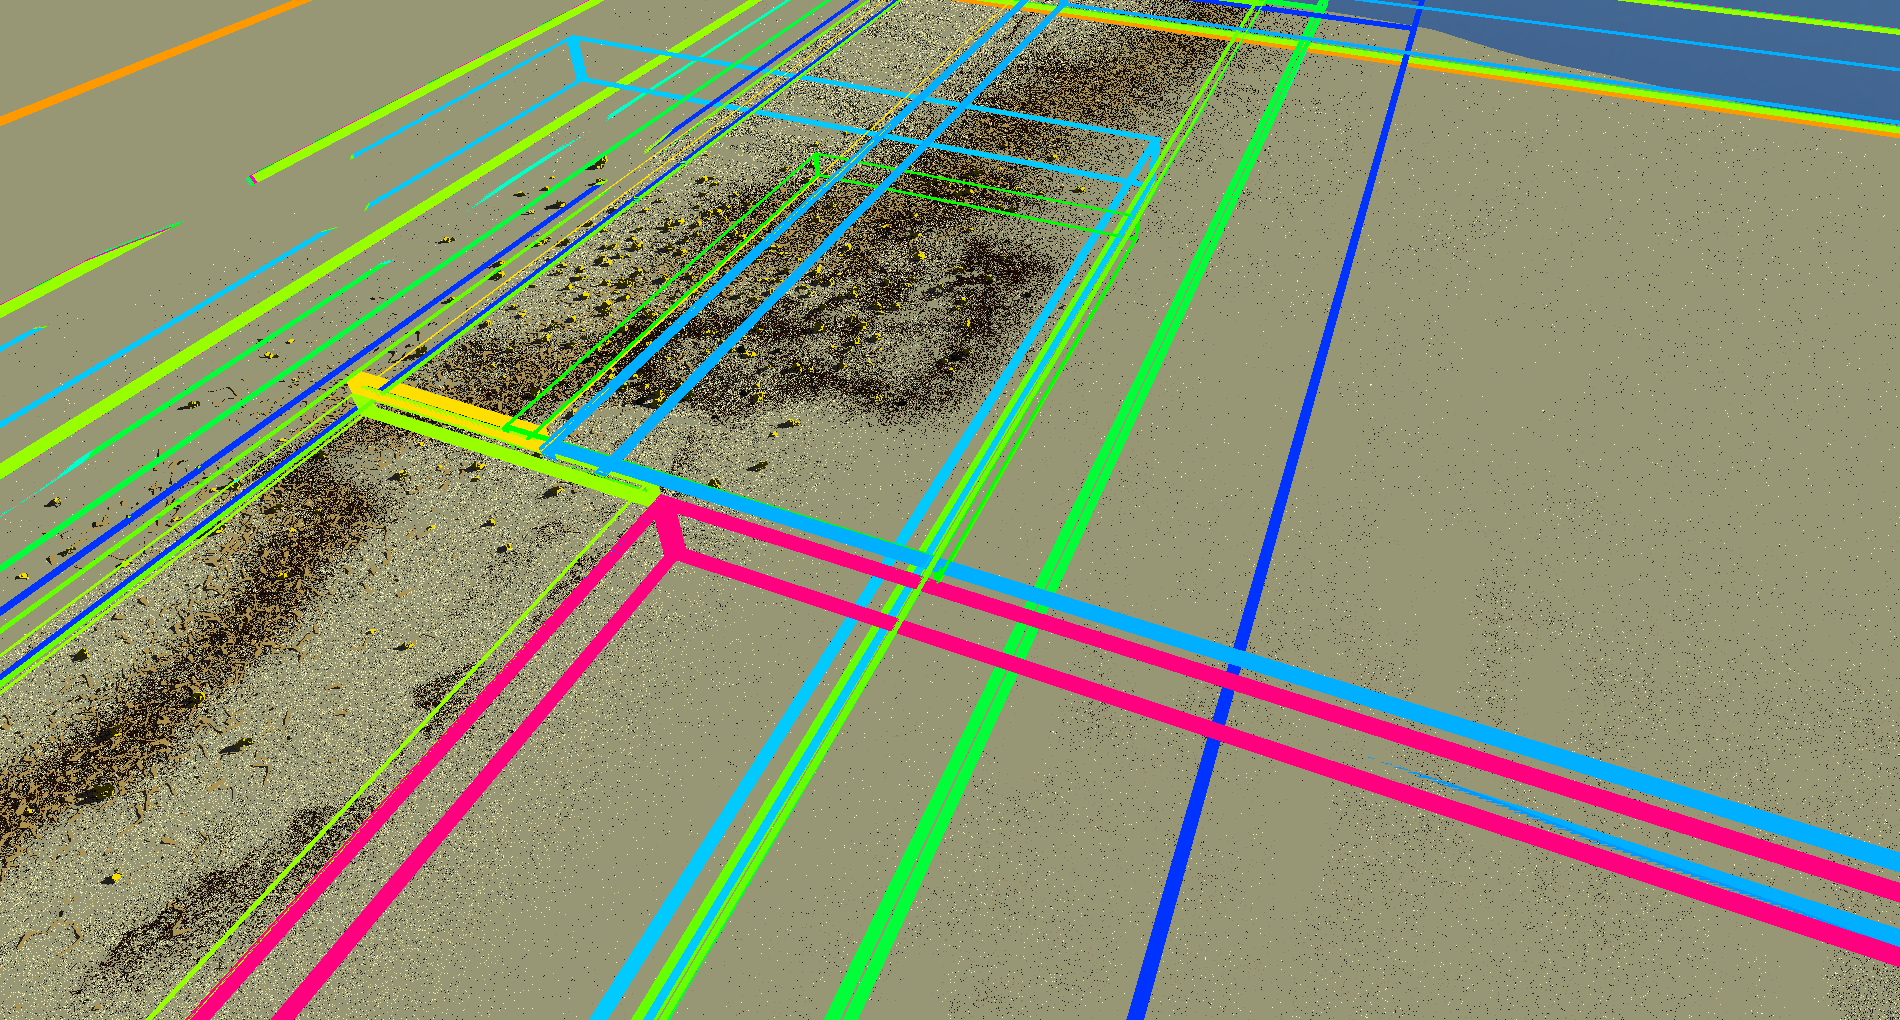
\includegraphics[width=.5\textwidth]{images/showcase/BeachUnmerged.PNG}}
\subfigure[Processed AABBs]{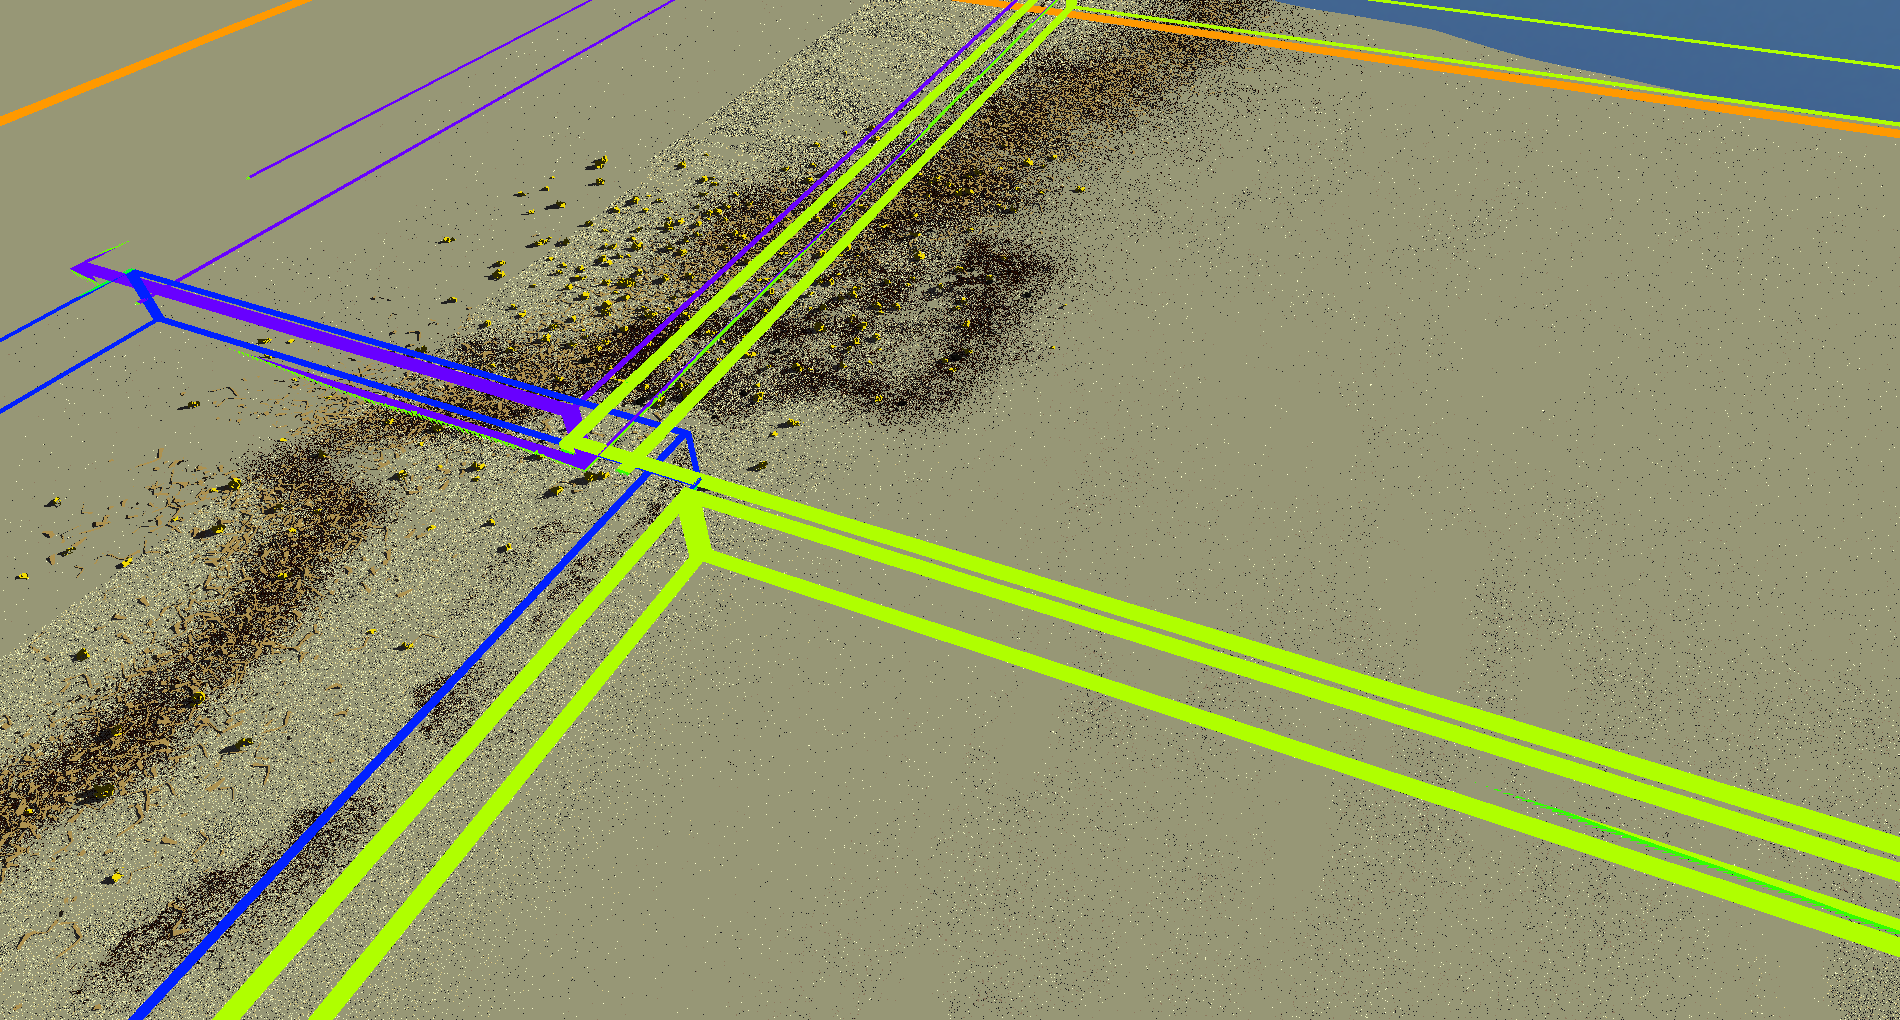
\includegraphics[width=.5\textwidth]{images/showcase/BeachMerged.PNG}}
\caption{Beach Moana Island, 24M instances requires split.}
\label{fig:isBeachFigure}
\end{figure}
Figure \ref{fig:isBeachFigure} shows a case where it is required to split instances, as there are lot of small rocks inside that scene ($\approx 20M$). In fact, these are more instances than the GPU supports inside an acceleration structure. Therefore, it is necessary to split the AABBs into smaller ones. Using a median split delivered sufficient results with only a low AABB overlap. A small AABB overlap is essential for the performance of raytracing, since the AABBs determine which path the traversal takes. If two AABBs overlap traversal needs to traverse both sub-trees, which results in an increase in traversal time.\\
In the best case, traversal time takes the trees height (O(log(n)). For unbalanced trees or with large AABB overlap it can be O(2n) = O(n), since the number of AABBs is at maximum the number of primitives. Then every leaf must be traversed.\\
For GPU traversal, acceleration structures are using optimized BVHs. These prioritize one of the following values.
\begin{itemize}
    \item Construction time - most of the time during construction is spent by sorting primitives into the sub-trees. Using a faster split heuristic results in faster build times. Increasing parallelism can also be of help here. 
    \item Traversal time - the most common case, since this is the one that mostly improves framerate. Traversal time is improved by keeping the tree balanced and minimizing AABB surface along the split axis.
    \item Memory usage - low memory means less AABBs and more children per node. This goes for leaves as well as the number of sub-trees inside a node.
\end{itemize}
\newpage
\subsection{Octree}
\label{sec:Octree}
\begin{figure}
    \centering
    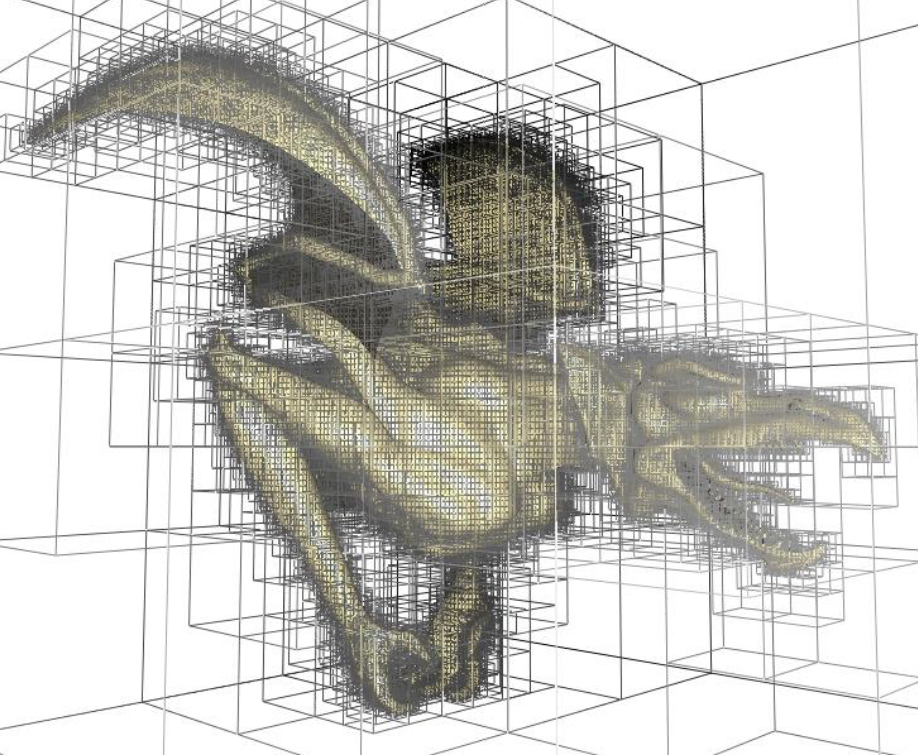
\includegraphics[width=.5\textwidth]{images/showcase/Octree Lefebvre 2004.PNG}
    \caption{Octree for a triangle mesh [Lefebvre 2004].}
    \label{fig:Octree}
\end{figure}
The octree is a grid-based layout. It separates space into sections that do not overlap. Its goal is to keep shrinking the section size until it only contains a predefined maximum of primitives. Octree hereby refers to the number of children that each node in the tree has. An octree therefore has eight children per division. Two for each of the three dimensions. At first the section is large enough to encapsulate the entire scene. After that the nodes keep being divided until only a maximum number of primitives is left. This can be seen in figure \ref{fig:Octree}. A common division axis is the middle point of the extent of the node to be divided. It is also possible to use other ratios and might even improve performance significantly. For evenly distributed geometry the tree reaches a height of $O(log(n))$ resulting in logarithmic traversal times. However, there are cases where the geometry is very dense in a small space. Then the trees height grows quickly up to O(n).\\
Octrees have some advantages when it comes to neighborhood searches, i.e. finding a point in space that is close to another without searching through every point in space. This makes them useful for computing intersections in physic engines.
\subsection{Usage}
Even though Nvidia does not specify which acceleration structure they are using on their GPU, in fact, they are using BVHs \cite{nvidiaTuringArchitecture}. In terms choosing the type of the acceleration structure to execute on card ray traversal it does not make a difference. The application can expect $O(log(n))$ traversal times. So, for this thesis we use BVHs with AABBs. In terms of generality it could really be any type of acceleration structure that has hardware support.
\newpage
\section{Modern GPUs}
\label{sec:GPU}
\begin{figure}
    \centering
    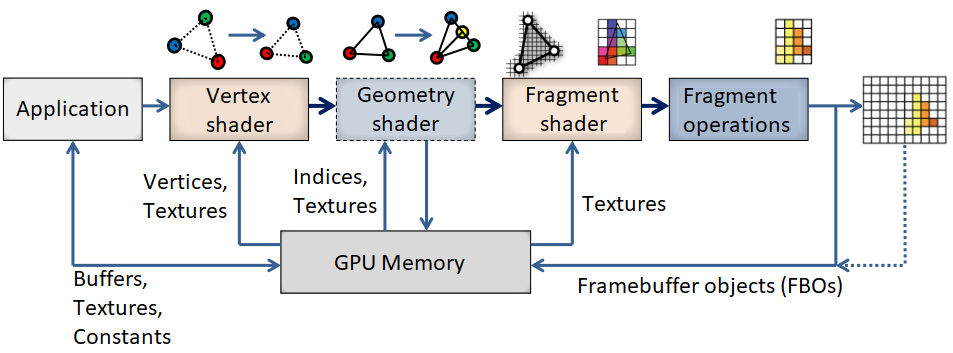
\includegraphics[width=\textwidth]{images/showcase/cgModernGPUPipeline.PNG}
    \caption{Rasterization pipeline. Source:cgLecture@KIT.}
    \label{fig:RasterizationPipeline}
\end{figure}
GPU, short for Graphics-Processing-Unit, is in fact just a very specialized form of multiprocessor CPU. It has a high emphasis on parallel computation, pipelining, and graphics computations. For example, an Nvidia GPU CUDA Core uses 32 Warp slots, which corresponds to 32 parallel executed threads \cite{nvdiaCudaGuide}. A GPU Streaming Multiprocessor executes instructions for each slot in parallel and a GPU can have a thousand of these cores. This makes for high performance for simple tasks that can be executed in parallel, for example computing the colors of a pixel on the screen. In addition to that, the general API of GPUs is highly focused around pipelining GPU operations, especially for rasterization. Figure \ref{fig:RasterizationPipeline} shows such a pipeline.
A modern GPU rasterization pipeline is commonly built as follows:
\begin{enumerate}
    \item Application - is the start point of any pipeline execution. It defines the inputs, global variables, shader programs, pipeline configuration and more.
    \item Vertex shader - is responsible for transforming 3D vertices by multiplying matrices onto them using homogeneous matrices provided by the application.
    \item Geometry shader - operates directly on a primitive and can discard, keep or even multiply it.
    \item Fragment shader - colors color fragments by computing shadows and reading in textures, then passes them on.
    \item Fragment operations - combines the color fragments for a pixel based on different rules. The Z-Test is the most used. It is responsible to bring the fragment in front which has the lowest depth i.e., is closest to the observer.
\end{enumerate}

Shaders are small programs specified for the pipeline to transform primitives through application defined functions \ref{sec:Shader}. 

Between the shader stages there are different inbuilt pipeline functions. These include:
\begin{enumerate}
    \item Clipping - dissects or discards triangles that are partially or fully outside of view.
    \item Tessellation - creates triangles by subdividing them to achieve higher resolution.
    \item Rasterization - creates a color fragment for each pixel that a triangle occupies.
\end{enumerate}

The newest of GPUs also have features that allow hardware accelerated calculation for more complex tasks, which results in a massive performance boost.\\
The best example for this are ray queries \ref{sec:VkRayQuery}, where a ray is shot into the scene and traverses an acceleration structure. This traversal process from the outside is quite simple.
\begin{lstlisting}
RayQuery rayQuery
initRayQuery(rayQuery, origin, minT, direction, ..., maxT)
while(rayQueryProceed(rayQuery)){
    //process the intersection, commit or discard
}
//Handle closest committed intersection
\end{lstlisting}
First up is initializing the ray query with a ray origin, ray direction and in what range intersections are accepted. Then a loop runs until the ray query is finished. In each iteration, the shader is then able to access the ray query data and either confirm or discard the intersection candidate.
The ray query runs while there are primitives left that have an intersection point lower than the currently best intersection. New GPUs support acceleration structure traversal with inbuilt hardware, called ray tracing cores. These make real-time applications possible that use raytracing on a large scale, like this thesis.

\section{Vulkan}
\label{sec:Vulkan}
\begin{quote}
    "Vulkan is a new-generation graphics and compute API for high-efficiency, cross-platform access to GPUs. As the industry’s only open standard modern GPU API, Vulkan is unique in enabling developers to write applications that are portable to multiple diverse platforms. Vulkan includes the latest graphics technologies including ray tracing and is integrated into NVIDIA’s production drivers for NVIDIA GeForce ..."\cite{vulkanNvidia}
\end{quote}
Vulkan is a graphics API by the Khronos Group with a large focus on a precise abstraction of modern graphics cards. This this confers much more control on the developer over his applications at the expense of having to put in a lot more work. It is most suitable for high performance graphics. In this chapter any noun that starts with Vk is a Vulkan struct, for more information about these structs I recommend either Vulkan-Tutorial \cite{vulkanTutorial} or the official Vulkan-Specification \cite{vulkanSpec}.
\subsection{Basics}
\label{sec:VkBasics}
The start for any Vulkan application is the VkInstance. It represents the connection between the application and the Vulkan library. To create a VkInstance it is required to specify API, engine, and application version as well as their names. Instance extensions, for example, using GLFW with Vulkan, must also be defined.\\
Debugging graphics applications can be quite bothersome as well as performance hindering. To this end Vulkan introduced a layer concept that can be toggled on or of depending under what configuration it is currently running (Debug/Release). The best example is the Validation Layer, which is provided by the LunarG-Vulkan-SDK. It performs parameter checking, thread safety, memory leak checks and more. This can be enabled during development and can later be removed at almost no performance cost when releasing the application.\\
VkPhysicalDevice and VkDevice are the next step when working with Vulkan. The Physical device represents the actual graphics hardware device that Vulkan will use.\\
The VkDevice represents the logical device that abstracts from the physical device and provides the working context. When creating the VkDevice the application also specifies the required device extensions. In this thesis the ray tracing extensions are required, which will limit the software to devices (GPUs) that offer the required support. Most notably the RTX family from Nvidia.
\subsection{Presentation}
\label{sec:VkPrensentation}
Presentation requires a VkSurface, it can be provided with by a GLFW window, which in turn interfaces with the Native-Window depending on the executing operating system. Each VkPhysicalDevice also supports different queues, one of these can be the Graphics and Compute queue that is also able to present images onto the screen. An application should retrieve a VkQueue handle, as it is the entry point to issue commands to GPU. Submitted commands are then taken from the queue and executed.\\
The VkSwapchain is an abstraction of the process of rendering to a framebuffer and then presenting on the screen. For its creation it requires setting the image format, presentation mode, surface VkExtent and a max VkImage count. The VkImage count corresponds to the amount of VkFramebuffers that can be exchanged for image presentation, typically two.\\
Once the VkSwapchain is created, the application can retrieve the VkImages that are used for drawing and presentation\\
Last are the VkImageViews, which quite literally allow the program to access specific parts of an image object.
\subsection{Shader}
\label{sec:Shader}
Shaders are executable programs that can be used inside certain pipeline stages. They operate on a certain input and produce an output which can then be passed to other pipeline stages. They are normally written in a human-understandable language, compiled and as bytecode specified for GPU pipeline. One such language is GLSL, and it will be used throughout this thesis. An example for a shader would be the vertex shader that transforms vertices and modifies their properties according to the program code. It for example transforms them from model to projection space by using a transform \ref{sec:transformations}. Shaders have access to the input, output, and global values. The latter being buffers, uniforms and other descriptors.\\
VkDescriptors are a way of defining what buffers, structs and data-structures are accessible to a shader. They each have a binding for these values. Using these bindings applications can then bind the relevant resources to the various descriptors.\\
A classic example for this are textures inside a fragment shader. To shade a pixel, a texture must be read and sampled. For this purpose, a shader must define a texture sampler as well as a texture image. GLSL also allows to combine these two. These must be specified on VkPipeline creation. Before the drawing process starts the application binds the relevant texture and sampler for each mesh it processes. Typically different meshes use different textures. Therefore, a valid approach would be to first bind texture1 for mesh1 and render it and after that binding the texture2 for the mesh2 and rendering it afterwards. However note, that this is not the only approach to this problem, as it is also possible to assign a descriptor for an array of textures that does not require setting a new binding before each draw command. This is also useful for meshes that use multiple textures.\\
Shaders represent the most configurable stages of the pipeline and depending on framework and type must be specified by the application. The execution code can be arbitrary as long as if follows the language specifications and cannot use recursion.
\subsection{Pipeline and Renderpass}
\label{sec:VkPipeline}
The VkPipeline specifies how the GPU pipeline is configured and which shaders and VkDescriptors are used. It also specifies the used fixed functions and how they are configured. The VkPipeline configuration is very flexible and taking a look at all the available settings is definitely worth it. Shaders are passed in Spir-V bytecode. VkDescriptor layout and their bindings are represented with a VkDescriptorSetLayout.\\
The VkRenderpass is responsible for containing the render information. It wraps around the pipeline to define a single draw operation in its whole. Furthermore, it specifies the attachments that are used for rendering, such as images. A VkRenderpass can be seen as one pass through a pipeline, they can also be chained.\\
It is for example possible to define multiple renderpasses, like a visibility and a shading pass to use benefits of rasterization and raytracing \ref{sec:RayRasterUsage}
\subsection{Framebuffers}
\label{sec:VkFramebuffer}
VkFramebuffers represents an image as an attachment for a VkRenderpass. An example is the color attachment for a standard framebuffer.
\subsection{Command Buffers}
\label{sec:VkCommandbuffer}
Command buffers are the principal component when passing work onto the GPU. They are used to record commands and then submitted so Vulkan can process them more efficiently.
\section{Scene graphs}
\label{sec:SceneGraph}
\begin{figure}
    \centering
    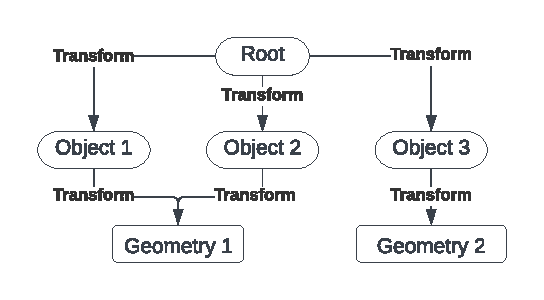
\includegraphics[width=.5\textwidth]{images/showcase/Scenegraph.pdf}
    \caption{A scene graph built out of objects with transforms.}
    \label{fig:SceneGraph}
\end{figure}
Representing a scene graph on a low level with a low memory usage can be quite bothersome, as well as creating a scene in memory from a text file that contains human readable text. When using Vulkan it is advantageous to use a low-level language like C++ or C since explicitness is a main goal of Vulkan. However, many high-level functions for parsing files and optimizing a scene layout are difficult to implement on a low level. For this thesis a static scene is used. This makes it possible to precompute all data necessary for the scene in advance. Furthermore, parsing text files like gltf-embedded for general scenes or .pbrt files for Moana Island requires a lot of time, since they contain text. The way to save the scene would therefore be a byte file. On its advantages it is beneficial to read the blog for the ToyRenderer from \cite{momentsingraphics}. An example for a scene graph can be seen in figure \ref{fig:SceneGraph}
\subsection{Parsing}
First stage is reading the files and putting them into the scene format that was specified. Some tasks can be executed in parallel for example reading in files. Here, high-level functions are advantageous as well as garbage collection. This makes life a lot easier.
\newpage
\subsection{Scene Buffers}
\label{sec:SceneBuffers}
In the common case multiple buffers are required to fully describe a scene. For the purposes of this thesis the following buffers are used:
\begin{itemize}
    \item Vertex Buffer - the 3D coordinates, 3D normal and texture coordinates. A vertex also specifies its used material.
    \item Index Buffer - 3 vertices represent a single triangle.
    \item Node Buffer - the nodes of the scene graph
    \item Transform Buffer - the matrix transforms used by the nodes
    \item Children Buffer - the relations between nodes in the scene graph
    \item Material Buffer - the materials with their lighting properties in addition with the referenced texture
    \item Light Buffer - the lights throughout the scene
\end{itemize}
\subsection{Optimization}
\paragraph{Instancing}
\label{sec:instancing}
Instancing allows to duplicate meshes throughout the scene by inserting multiple scene nodes that all reference the same geometry mesh. This leads to the same mesh appearing multiple times throughout the scene with different location, rotation, and scaling. We can instance the same scene graph multiple times for creating multiple levels of instancing. An example can be seen for Geometry1 in Figure \ref{fig:SceneGraph}
\paragraph{Level of Detail}
\label{sec:LOD}
Level of detail (LOD) is a technique that creates different versions of the same mesh with different resolutions. For this the vcglib\cite{vgcLib} is used, which supports reducing triangle meshes and interfaces with the scene compiler with .ply files and the command line. However, the Tridecimator does not allow for material indices. Instead, the material index is regarded as vertex color when creating the ply file and is preserved throughout the conversion. This is due to a mesh consisting of multiple submeshes that have different materials. This makes it necessary to preserve the material indices during conversion.
\newpage
\paragraph{Reordering}
\label{sec:Reorder}
Having the scene nodes in an arbitrary order also leads to random accesses,  that correspond to low cache hit rates. Therefore, the scene nodes are reordered designed in such a way, when using a depth search through the tree the children of a node children are close in memory. In doing so caching should be improved when traversing the scene for triangle intersections. Let C(n) denote the children of a node n, we initialize all indices with -1. Set the root.Index=0 and call this function for it.
\begin{lstlisting}
int asignIndices(Node n, int offset){
    if(C(n).length = 0)
        return offset
    start <- offset
    foreach(Node c in C(n)) {
        if(c.Index<0){
            c.Index <- offset
            offset++
        }
    }
    if(start=offset)
        return offset
    
    foreach(Node c in C(n)) {
        offset = assignIndices(c,offset)
    }
    return offset
}
\end{lstlisting}
Let us quickly analyze this function. As explained in the previous section \ref{sec:BVH}, an acceleration structure traverses a tree in a depth-first search that always resumes at the AABB with the lowest t-Value. In turn, this requires the calculation of every child's AABB intersection t and therefore access to their data. Furthermore, they will be accessed arbitrarily.\\
This assignment now works on two different assumptions:
\begin{enumerate}
    \item When a node is accessed, all children are probably too. Therefore, a child should always be near its parent.
    \item When a node is accessed, the search will resume in a Depth-First-Search, which corresponds to all sub nodes of this node being contained in its own sub range inside the buffer.
\end{enumerate}
While this is certainly not optimal, for repetitive instancing patterns, it guarantees that all children are quite close to the parents.
\paragraph{Further Optimizations}
The scene graph can then be passed into a processing step that does some operations like removing unused or empty nodes, grouping, and dividing based on some experience during the development. I will talk about this later in more detail as the problems are arising.
\subsection{Writing}
The writing process converts these objects into byte arrays and prepend the count of them before them. The layout matches exactly the structs used by the rendering application in C. This results in quite an easy and fast loading of the scene. It just reads the amount objects, allocates a buffer and copies the file contents into it.
\chapter{Raytracing with Vulkan}
\label{sec:VkRayTracing}
Since early 2018, the Khronos Vulkan Ray Tracing Task Sub Group (TSG) has been working on adding extensions so the Vulkan framework. After two years of work, the Ray Tracing TSG released these new features with the announcement of the Vulkan SKD 1.2.162.0. Due to the extension structure that Vulkan is based on, the extensions integrated quite easily into the Vulkan API.
\begin{quote}
    One overarching design goal was to provide a single, coherent cross-platform and multi-vendor framework for ray tracing acceleration that could be easily used together with existing Vulkan API functionality.
\end{quote}
This was made possible by the very explicit nature of Vulkan which gives the user, and the extension developers sufficient control.\\
The Vulkan ray tracing functionality introduced a number of Vulkan, SPIR-V and GLSL extensions, which allows applications access to these new features. These include:
\begin{itemize}
    \item Vulkan extensions
    \begin{itemize}
        \item VK\_KHR\_acceleration\_structure \ref{sec:VkAccelrationStructure}
        \item VK\_KHR\_ray\_tracing\_pipeline \ref{sec:VkRayPipe}
        \item VK\_KHR\_ray\_query \ref{sec:VkRayQuery}
    \end{itemize}
    \item GLSL extensions
    \begin{itemize}
        \item GLSL\_EXT\_ray\_tracing \ref{sec:VkRayPipe}
        \item GLSL\_EXT\_ray\_query \ref{sec:VkRayQuery}
    \end{itemize}
\end{itemize}
Of particular interest to us, are VK\_KHR\_acceleration\_structure, GLSL\_EXT\_ray\_query. The first one allows us to create VkAccelerationStructures that reside on the GPU. Furthermore they also allow for hardware accelerated traversal, which benefits ray tracing significantly \ref{sec:BVH}. The latter is the extension needed to use acceleration structures inside a GLSL shader. \cite{vulkanRayTracing}
\newpage
\section{Vulkan Acceleration structures}
\label{sec:VkAccelrationStructure}
The Vulkan acceleration structure features two types of acceleration structures: Top-Level-Acceleration-Structure (TLAS) and Bottom-Level-Acceleration-Structure (BLAS). Together they form a 2 Level hierarchy. Each acceleration structure is built over a number of geometries (VkAccelerationStructureGeometryKHR).

\begin{figure}
    \centering
    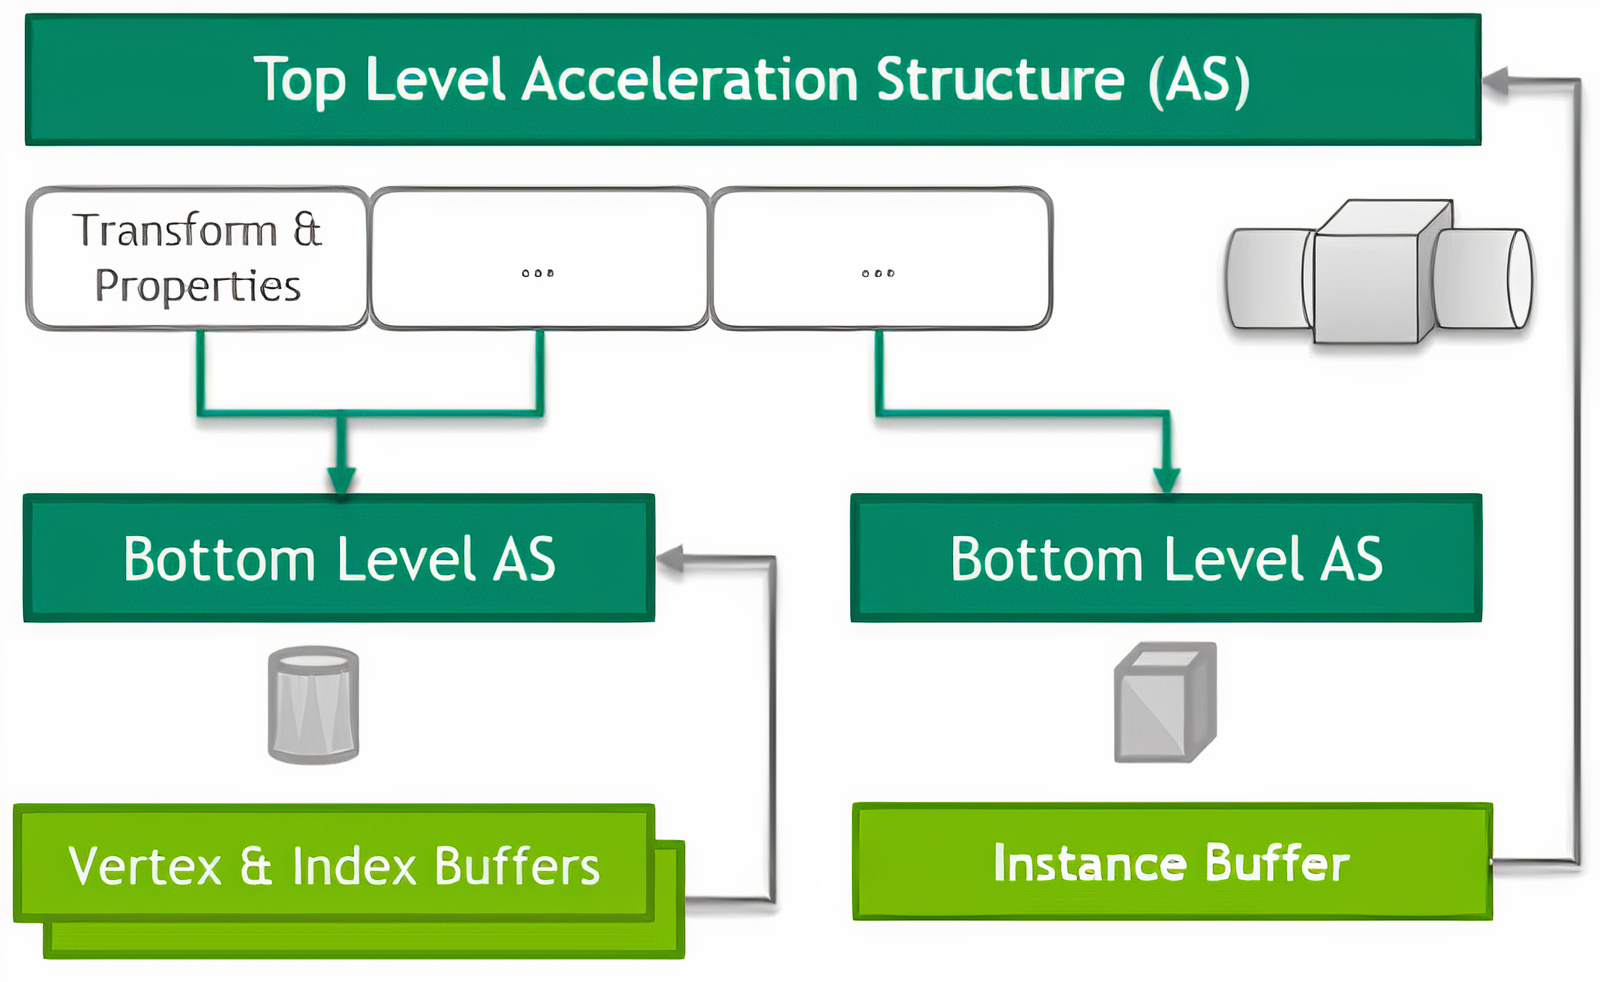
\includegraphics[width=.8\textwidth]{images/showcase/accelerationStrucutres.jpg}
    \caption{Layout of acceleration structures in Vulkan \cite{vulkanRayTracing}.}
    \label{fig:VkASLayout}
\end{figure}
 
A TLAS includes only instances (VkAccelerationStructureGeometryInstancesDataKHR, VkAccelerationStructureInstanceKHR), which corresponds to BLAS references with a transform and specific properties. Basic examples for this would be trees in a forest. The trees are BLAS which contains the trunk, branches as well as the leaves. Then they are instanced as a whole and distributed throughout the scene. Each instance having its own translation, rotation and scale, in short with a $4\times4$ homogeneous matrix. Together with the BLAS references they create an instance. Multiple of these form the top level geometry. Vulkan allows us to give each instance a custom index. This will be useful later, when we try to find out which instance we actually intersected.\\
A BLAS consists of either triangles (VkAccelerationStructureGeometryTrianglesDataKHR), AABBs (VkAccelerationStructureGeometryAabbsDataKHR, VkAabbPositionsKHR) or a combination of the two. Triangles can be passed by using either only positions or using positions and and index buffer. AABBs are specified with their own transform, with a min and max vector.\\
Vulkan does not give access to a custom index here. We will have to rely on the actual index and therefore the order in which we passed the geometry into the acceleration structure build.
\cite{vulkanRayTracing}
\newpage
\section{Acceleration structure construction}
\label{sec:VkASBuild}
The construction process follows the usual Vulkan principle of explicit commands. The basics steps are as follows.
\begin{enumerate}
    \item Create the VkAccelerationStructureBuildGeometryInfoKHR, by allocating buffers for the build and copying the contents into them. It is also possible to use already present vertex and index buffers and then specifying a range for the build. The same principle applies to AABB or Instance Geometry.
    \item Determine the VkAccelerationStructureBuildSizesInfoKHR with vkGetAccelerationStructureBuildSizesKHR(). It contains the required acceleration structure size and build scratch size. The latter being a buffer that the GPU uses for storing data while constructing the acceleration structure. The buffers are then created with the relevant sizes.
    \item Create the VkAccelerationStructureKHR by specifying type, properties, geometry and optionally a build Range and calling vkCreateAccelerationStructureKHR().
    \item Build the acceleration structure by recording a command buffer with a vkCmdBuildAccelerationStructuresKHR() command, then setting a pipeline barrier to re-synchronize the CPU with the completion of the acceleration structure build.
\end{enumerate}
When using ray tracing it is also necessary to specify a descriptor for the acceleration structures. They are created in the same way other descriptors are made. Specify the binding in the descriptor set layout and later creating and updating the descriptor set. Lastly bind the descriptor set to the command buffers \cite{vulkanSpec}.
\newpage
\section{Ray Tracing Pipeline}
\label{sec:VkRayPipe}
\begin{figure}
    \centering
    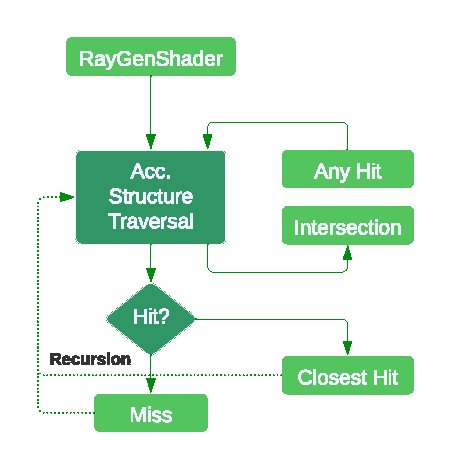
\includegraphics[width=.6\textwidth]{images/showcase/RayPipeline.pdf}
    \caption{Vulkan Ray Tracing Pipeline \cite{vulkanRayTracing}}
    \label{fig:VkRayPipeline}
\end{figure}
One of two ways to use raytracing in Vulkan is using the newly introduced ray tracing pipeline. Which follows the same principles as the traditional rasterization, with a focus on high parallelism and independence of rays, which leads to good usage of GPU resources and with driver/API managed pipeline operations. \\
The pipeline introduces a couple of new shader stages. First up is the ray generation shader, which is used to generate rays and execute raycasts into the scene and finally setting the color of the pixel. Casting rays is done by using GLSL\_EXT\_ray\_tracing with the function traceRayEXT().\\
The closest hit shader gets executed for the closest intersection that the raycast computed, if there was one. Here the shader can either return a value or for example compute transmission, reflection, and other coefficients, by using recursion and tracing more rays.\\
The miss shader is for the case, that a ray does not hit any geometry whatsoever. If this is the case one could return a constant color or fetch the color from an environment mapping with a skybox.\\
Any hit and intersection shaders can modify traversal by discarding hits or computing custom t values for AABBs, one use case for this is raytracing spheres.\\ \cite{vulkanRayTracing}
\newpage
\section{Ray Queries}
\label{sec:VkRayQuery}
Another way of using raytracing is ray queries. Instead of introducing a new pipeline layout, this extension integrates raytracing functionality into the existing rasterization layout. Which can be used to profit from the main advantage that comes with raytracing, that being realism. It allows for very accurate shadows, reflections and transparency while only adding minimal implementation overhead inside the shader.
\begin{figure}
    \centering
    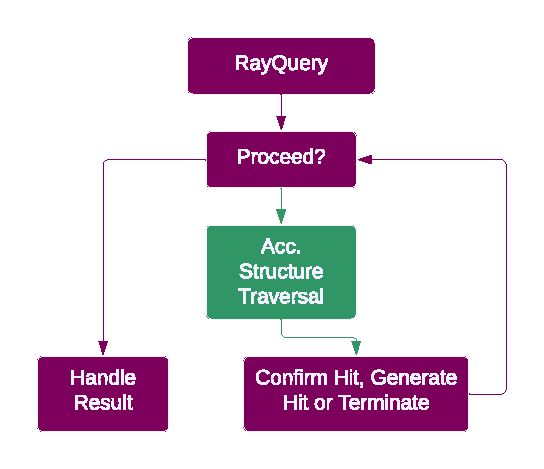
\includegraphics[width=.6\textwidth]{images/showcase/RayQuery.pdf}
    \caption{The Vulkan ray query loop \cite{vulkanRayTracing}}
    \label{fig:VkRayQuery}
\end{figure}
The general structure follows a simple while loop, which looks like this when Using GLSL:

\begin{lstlisting}
rayQueryEXT rayQuery;
rayQueryInitializeEXT(rayQuery, accelerationStructure,
                      flags, cullMask, origin, 
                      tMin, direction, tMax);

while(rayQueryProceedEXT(rayQuery)) {
    if (rayQueryGetIntersectionTypeEXT(rayQuery, false) ==
        gl_RayQueryCandidateIntersectionTriangleEXT)
    {
        ... // Determine if an opaque triangle hit occurred
        if (opaqueHit) rayQueryConfirmIntersectionEXT(rayQuery);
    }
    else if (rayQueryGetIntersectionTypeEXT(rayQuery, false) ==
             gl_RayQueryCandidateIntersectionAABBEXT)
    {
        ... // Determine if an opaque hit occurred in an AABB
        if (opaqueHit) rayQueryGenerateIntersectionEXT(rayQuery, ...);    
    }
}

if (rayQueryGetIntersectionTypeEXT(rayQuery, true) ==
    gl_RayQueryCommittedIntersectionNoneEXT)
{
    // No hit!
} else {
    // Hit!
}
\end{lstlisting}
\cite{vulkanRayTracing}

Line 1 declares a RayQuery GLSL construct, which is then initialized in line 2.
As parameters, the ray query uses the struct as well as an acceleration structure to traverse.
Furthermore, the RayQuery requires a ray origin as well as a direction. tMin and tMax specify which range of intersection t values are allowed, with tMin being the minimum distance the ray hits an object from the origin. tMax is the maximum distance.\\
Line 7 starts the traversal loop. This function returns true for as long as there are any remaining intersections to process.\\
Following this is an if-else statement differentiates which type of intersection took place. With triangle intersections having predefined functions that can extract the appropriate t-value, UV-coordinates and more. For a triangle candidate to be regarded as an intersection it is necessary to confirm the intersection using the function in line 11. The available functions for processing triangle intersections are the following:\\
\begin{enumerate}
    \item rayQueryGetIntersectionTEXT - returns the t value for a triangle intersection
    \item rayQueryGetIntersectionBarycentricsEXT - returns the barycentric coordinates of a triangle hit
\end{enumerate}
When intersecting AABBs the developer must define such functions themselves, as well as the actual intersection test. A basic example for this is raytracing spheres. The application inserts a call to an intersection function to determine whether the sphere was actually intersected by solving a quadratic. For obtaining sphere data, or in more general the data for which type was intersected, the application has to rely on the following functions:\\
\begin{enumerate}
    \item rayQueryGetIntersectionInstanceCustomIndexEXT - for every instance it is possible to define a custom index which can be read for an intersection. This value can in theory be any 32bit value and type, it just has to be cast back to the appropriate type. In our case this will be used as an index into a buffer which directly provides us information about which instanced geometry was actually intersected.
    \item rayQueryGetIntersectionPrimitiveIndexEXT - since a BLAS contains multiple geometries this index provides the position of the geometry in the order it was specified when creating the acceleration structure (VkAccelerationStructureGeometryKHR). There is no custom index available for retrieving the actual primitive.
    \item rayQueryGetIntersectionInstanceShaderBindingTableRecordOffsetEXT - this is used when using the raytracing pipeline. It specifies which shader to execute in the shader table when intersecting primitives in this BLAS. However, it is possible to use this value another way when using ray queries since it is unused in that case. For our purposes we use this value to access another index into a buffer.
    \item rayQueryGetIntersectionInstanceIdEXT - this is the equivalent for rayQueryGetIntersectionPrimitiveIndexEXT, it just returns the index of the instance for the geometry of the TLAS.
\end{enumerate}
When taking the sphere example further, one could imagine a scene node which references n spheres. When creating a BLAS for this node we add the spheres in the same order as they are the nodes children. With the custom index we can identify this node and retrieve it form the buffer. Since the node is an application defined struct, the application can set flags on it. For example, indicating that the children of this node are spheres.\\
With this information the index of the sphere can be determined using the primitive index. It is then possible to retrieve the appropriate structs with the node and the sphere index. This struct then contains a radius as well as a position value, which then can be used to run an intersection test by solving a quadratic equation. Once this has completed what remains is either deciding whether the intersection actually occurred or not. If it did, then the computed tValues are used to generate an intersection at the smallest value that is bigger than tMin.\\
Lastly, once there are no intersections the closest hit is processed. Determine which type of hit occurred, if any. Then finally implement different behavior to change fragment shading.\\
Note that intersection takes place in object space, for this the GLSL extension also provides methods to retrieve ray parameters in world and object space:
\begin{enumerate}
    \item rayQueryGetIntersectionWorldToObjectEXT - retrieves the transform into the coordinate system
    \item rayQueryGetIntersectionObjectToWorldEXT - retrieves the transform from object space to world space
    \item rayQueryGetIntersectionObjectRayOriginEXT - retrieves the ray position the objects coordinate system
    \item rayQueryGetIntersectionObjectRayDirectionEXT - retrieves the ray direction in the objects coordinate system
\end{enumerate}
The user also can terminate the ray query prematurely(rayQueryTerminateEXT) or specifying the any-hit flag which terminates the ray query as soon as either a triangle has been commited or an intersection was generated (gl\_RayFlagsTerminateOnFirstHitEXT). This method is useful for calculating light source occlusion.\\
Ray queries give a lot of control to the calling shader module; however they have a tiny disadvantage: Recursive ray-casts must be made explicitly using its own managed stack, because Spir-V does not allow recursive function calls. This makes them quite handy for computing shadows.\\
What might be worth trying when using ray tracing might be a combination of the two. Since ray queries do not suffer from the overhead that the pipeline does, they can be used to execute AnyHit raycasts to calculate light occlusion. While the pipeline is used for transmission and reflection.
\chapter{Traversal Shader Implementation}
\label{sec:ImplTraversalShader}
The acceleration structures that we currently have at our disposal are limited to two levels. Additionally, there is no option to execute a ray query on a bottom level in of itself. This does not allow for techniques like multi-level instancing, which inherently requires at least three levels. Neither is there any functionality to modify traversal while it is running. Most of the time this requires the scene to fit into one single acceleration structure. In most cases, this is fine, but in extreme cases for exceptionally large or detailed scenes (for example Moana Island) the use of level of detail and multi-level instancing is essential for performance and memory usage. Traversal shaders present a solution for this problem in a more general way. As mentioned before, the goal is to implement traversal shaders on GPUs that allow for multi-level instancing, dynamic Level-of-Detail and more on current GPUs, bypassing the two-level limitation. Won-Jong et al. \cite{traversalArticle} proposed a solution for this with their traversal shader, which we will try to simulate on a modern GPU that has ray query support.
\newpage
\section{Concept}
\label{sec:Concept}
\begin{figure}[h]
    \centering
    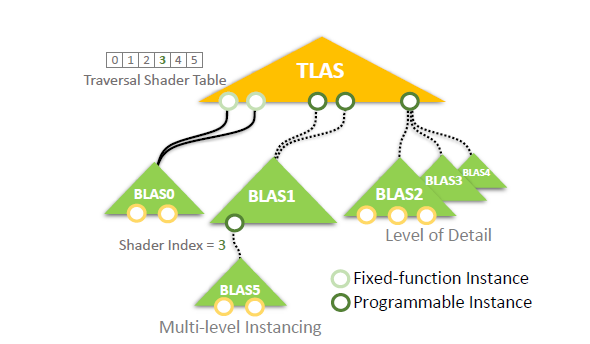
\includegraphics[width=.8\textwidth]{images/showcase/traversal hirarchy.PNG}
    \caption{Traversal shader structure \cite{traversalArticle}.}
    \label{fig:TraversalShader}
\end{figure}
Traversal shaders allow us to modify traversal dynamically (during execution) by inserting a new type of geometry, the programmable instance (PI). It behaves like an AABB, except when it is intersected by query, a shader is called, which is specified during the AS build. The state of traversal inside an acceleration structure can be described by a payload. The programmable instance shader has access to these payloads and can modify them. Therefore, it is able to influence along which nodes traversal resumes. Additionally, the shader can add a new payload on the top of the payload stack. This lets the traversal resume in the newly specified payload first before resuming with other payloads. Programmable instances can be referenced by both TLAS and BLAS. With the traversal shader Multi-Level-Instancing can be implemented by letting traversal continue into a lower-level BLAS \ref{fig:TraversalShader}.\\
As stated, with this model traversal can reach several levels deep. This requires keeping track of the state of traversal in all previous AS. To do this, a stack is required, which will be called traversal stack from here on out. This stack and its contents completely describes the state of traversal.\\
Note that halting and resuming traversal is bad for performance on the current architecture. Therefore, the traversal stack instead contains the acceleration structures that have to be traversed next in our implementation. More on that in the next section.\\
Figure \ref{fig:TraversalShader} shows a basic layout for application of traversal shaders. It features 3 different cases.
\begin{itemize}
    \item Left - This represents the current state. A TLAS instance references a single BLAS (BLAS0) and multiple instances can reference the same BLAS with different flags and transforms.
    \item Middle - shows the structure for multi-level instancing. Firstly, BLAS1 is instanced by using a PI-Shader that adds BLAS1 as a payload to the traversal stack and traversal resumes there. While traversal runs in BLAS1 it can intersect another PI that adds BLAS5 to the traversal stack. Traversal then resumes there before it finishes in BLAS1 and the TLAS.
    \item Right - shows the structure for Level-of-Detail. The PI in the TLAS makes the traversal execute a shader which invokes the selection of a Level-of-Detail to resume traversal. Since this code is executed during traversal, it allows for a dynamic selection of the LOD.
\end{itemize}
Note that traversal does not necessarily occur in this order. An alternate way of describing this traversal process might be a depth first search. When traversing a node, the children are added in ascending t value from the ray origin. The goal for this thesis is to emulate the traversal shader using the newly released Vulkan API and to flag nodes as PIs and implement different shader behavior based on a PIs flags.\cite{traversalArticle}\\
Figure \ref{fig:TraversalOrder} shows the difference in traversal order of the proposed model and our implementation. It is in regard to traversal finishing inside an acceleration structure. There are couple of differences:
\begin{itemize}
    \item The proposed model always finishes with 1 as opposed to ours who finishes with an arbitrary TLAS.
    \item Traversal of a TLAS always finishes all BLAS in its sub-tree before resuming with other TLAS.
    \item The order in which the intersections in 6 are found is reversed in our implementation. This is not optimal as the traversal should always continue with the first intersected PI. The solution to this is reversing the added payloads. See \ref{sec:OptTraversalSpeed}.
    \item In our implementation only BLAS can contain PIs as children, they let traversal continue into a TLAS. For example 2-BLAS to 4-TLAS.
    \item The maximum stack size in a) is the depth of the tree (4).
    \item The maximum stack size in b) is the maximum of all paths with the sum of PIs as children of BLAS along this path. In our example one such maximum path would be 1-2-4-6 and its sum of PIs would be $0+2+0+0=2$. This can grow significantly more than the size in a) and may lead to artifacts. See \ref{sec:BottleStackSize}.
    \item a) only traverses 1 TLAS and b) traverses 3 TLAS.
\end{itemize}
\begin{figure}
    \hfill
    \subfigure[Order:6-4-6-5-2-6-5-3-1]{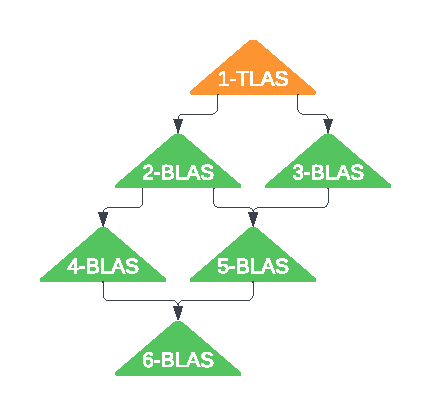
\includegraphics[width=.45\textwidth]{images/showcase/TraversalOrder - Model.pdf}}
    \hfill
    \subfigure[Order:2-3-1-6-5-6-5-6-4]{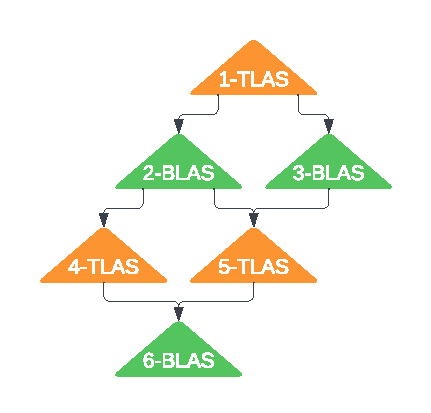
\includegraphics[width=.45\textwidth]{images/showcase/TraversalOrder - Impl.pdf}}
    \hfill
    \caption{The order in which traversal of acceleration structures finishes. Left: Order of the model proposed. Right: Order of our implementation. Intersections are assumed to happen from left to right.}
    \label{fig:TraversalOrder}
\end{figure}

\newpage
\section{Implementation}
\label{sec:Implementation}
As discussed in the Vulkan Raytracing Chapter, the API we are using does not support multi-level instancing, nor anything resembling a traversal shader. So, in this section we will work towards a pseudo-code implementation for the shader that we can translate into GLSL code. The GLSL implementation is presented in the last section of this chapter \ref{sec:FinalLayout}.
\subsection{Considerations}
\label{sec:Considerations}
Before starting with the implementation, let us summarize all that we know up to this point and start thinking about how to implement a traversal shader given the current limitations.\\
First, an acceleration structure consists of one TLAS and multiple BLAS. TLAS can only reference instances while BLAS can reference triangles and AABBs \ref{sec:VkAccelrationStructure}. There is also no apparent way of modifying traversal while it is running.\\
However, the application has the ability to execute arbitrary code for any given intersection. With this, PIs can be modeled as AABBs inside BLAS. Figure \ref{fig:TraversalHierarchy} shows the insertion of PIs into BLAS for different functionality. If a PI is then intersected the intersection data is then saved and processed later. Since PIs are geometry in a BLAS which is in turn referenced by a TLAS, it is required to have a way to retrieve the node that the PI belongs to. This can be solved by using the GLSL functions that retrieve index data for the RayQuery \ref{sec:VkRayQuery}. Thus, requiring to pass buffers to the shader that can retrieve nodes and their children.\\
The node is an application defined struct, which can be flagged in whatever way the application wants. This can be used to model different traversal shader behavior by using a switch statement.\\
\begin{figure}[hbp]
    \centering
    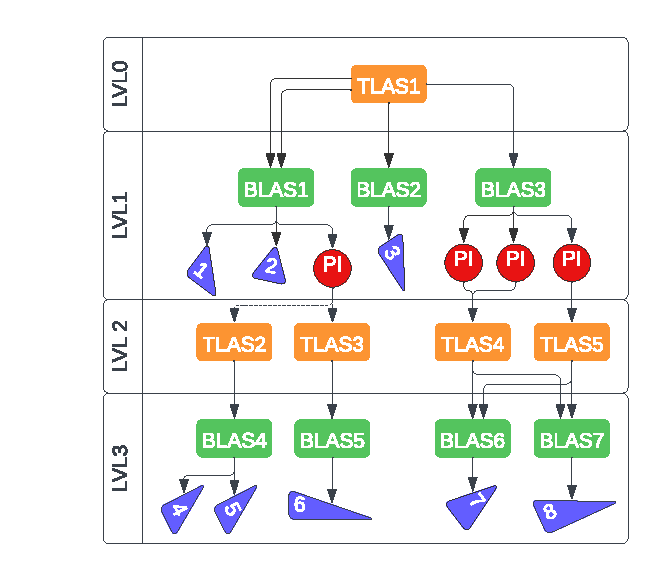
\includegraphics[width=.7\textwidth]{images/showcase/TraversalHierarchy.pdf}
    \caption{A traversal scene graph. Left: PI shows use of LOD. Right: Example for ML-Instancing.}
    \label{fig:TraversalHierarchy}
\end{figure}
\newpage
An intersection is processed inside the loop; however it is not possible to recursively call ray queries because GLSL does not allow for recursion. Thus, the best option is to traverse one acceleration structure after another.\\
To run traversal therefore requires a traversal stack. Any time a ray query intersects a programmable instance, a new payload is added onto the stack. This payload will then be executed at some point after the adding ray query has finished. Notice that every execution of a ray query could thus add to the stack. This makes a breadth-first-search unfeasible, since the size of this stack would always reach the maximum width of the tree at some point. This would make the stack use more memory than required. Therefore this makes a preorder-depth-first search the most feasible option, because it keeps the stack size as small as can be.\\
Every node can be contained inside an AABB. This is also the case for programmable instances. Therefore, any AABB for a programmable instance gives a lower and upper bound for any intersection t in its added payload. This can be taken advantage of to avoid traversing though payloads in which the lower bound is higher than the current best t-Value. This makes a DFS even more important, since it is likely that any geometry would be in the lower levels of the tree. This approach gives us an estimate for the t-Value faster than a BFS. Figure \ref{fig:TraversalStackTable} show an example for a tree traversal of \ref{fig:TraversalHierarchy}. The figure shows cases where a BLAS is intersected multiple times, the selection of a LOD with TLAS2 \& 3 and multi-level instancing with BLAS6 \& 7 as well as TLAS4. It also shows the ability to skip payloads if the current best intersection is before any possible intersection inside of a PI. Traversal finishes with query 6, since the stack is empty there.\\
To avoid a few edge cases, it is also beneficial to keep the relation between nodes. I.e., a TLAS can only reference BLAS and traversal can only start from a TLAS. It means: If we map the scene graph one to one to acceleration structures and a PIs only function would be to resume traversal into another TLAS, then it makes sense to assume every PI must be a TLAS. We can therefore split the scene graph into even nodes which can reference a TLAS and odd nodes which can reference a BLAS. Any node can only reference children with a different parity. To avoid edge cases this parity constraint will be carried on from here on out. Any odd-level node corresponds to a BLAS and every even-level node corresponds to a TLAS. This always gives the ability to map every node to an acceleration structure that only references its children and still obtain a valid and traversable scene graph.
\begin{figure}
    \centering
    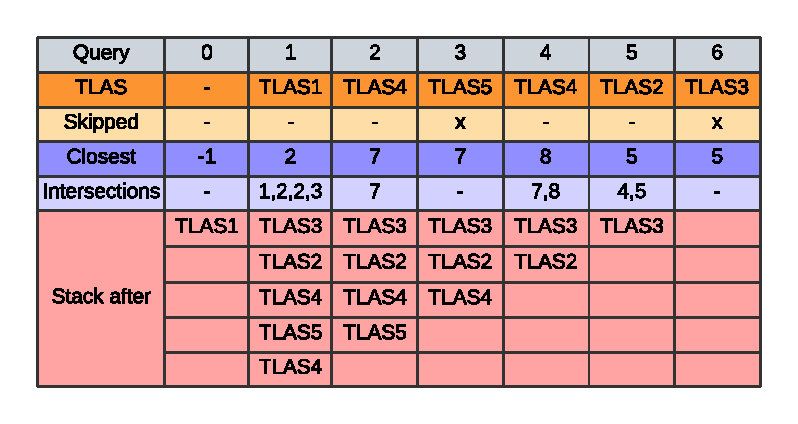
\includegraphics[width=.7\textwidth]{images/showcase/TraversalTable.pdf}
    \caption{Example of stack states during traversal of \ref{fig:TraversalHierarchy}.}
    \label{fig:TraversalStackTable}
\end{figure}
\newpage
\subsection{Scene Layout}
\label{sec:SceneLayout}
In this subsection I will describe the scene in a mathematical way. Section \ref{sec:SceneBuffers} and \ref{sec:Considerations} already gave an idea of which buffers and values will be required to access the data.
For traversal, a minimum of four buffers is needed, as well as an additional descriptor for the array of acceleration structures $\mathbf{TLAS}$.
\begin{enumerate}
    \item $\mathbf{V}$ - the Vertex buffer, with each vertex containing a 3-Dimensional vector representing Object-Space Position.
    \item $\mathbf{T}$ - the triangle indexbuffer, any triangle is identified by an Index $i$ with $0 \leq i<|\mathbf{T}|$ and $i = 0$ $\mathbf{mod}$ $3$. The three vertices that make up the triangle are $\mathbf{V}[i]$,$\mathbf{V}[i+1]$ and $\mathbf{V}[i+2]$
    \item $\mathbf{N}$ - the node buffer, it contains every scene node of the graph.
    \item $\mathbf{C}$ - the children indexbuffer, it contains indices $i$ into the node buffer with $0\leq i < |\mathbf{N}|$ that represent a node's children.
\end{enumerate}
Next, I will describe how the node and children index-buffer relate to each other.\\
The scene graph is a directed acyclic graph with a root node, which represents the entire scene. A node $n$ in the scene graph has a positive number of following children $c$ that have an edge from $n$ to $c$ in the graph. Since structs must always have a fixed size, the children of a node are obtained by accessing the node children buffer $\mathbf{C}$. To obtain the $i$-th child $c_i$ of $n$, use the child offset $C_{off}(n)$ of the node $n$ and 
\[c_i = \mathbf{N}[\mathbf{C}[C_{off}(n) + i]].\]
We also define the access to a node's triangles in a similar way. The vertices $v_0,v_1,v_2$ of the triangle $t_i$ are obtained with the IndexOffset $T_{off}(n)$ and
\[v_j = \mathbf{V}[\mathbf{T}[T_{off}(n) + i \cdot 3 + j]]\]
and
\[t_i = (v_0,v_1,v_2)\]
The triangles $T(n)$ of $n$ are therefore defined by the number of triangles $\#T(n)$, which is a value in the scene node struct, and
\[T(n) = (t_0,t_1,\dots,t_{\#T(n)})\]
\[T(n,i) = t_i\]
This also goes for the Children $C(n)$ of $n$, $\#C(n)$ with
\[C(n) = (c_0,c_1,\dots,c_{\#C(n)})\]
\[C(n,i) = c_i\]
We will also need to access some other Data for a node $n$:
\begin{itemize}
    \item I(n) - the index of the node inside the node buffer. $\mathbf{N}[I(n)] = n$
    \item L(n) - the level of the node in the scene graph
    \item M(n) - the objectToWorld transform as a homogeneous matrix $\mathbb{R}^{4\times4}$.
    \item B(n) - the AABB bounding box of the node that contains all children
    \item TLAS(n) - the acceleration structure index in the TLAS array descriptor, or -1 if the node has no TLAS
\end{itemize}
\subsection{Scene Constraints}
\label{sec:Constraints}
From the previous chapters, we know there are a few constraints that we must follow for our scene graph to use traversal shading. I will list all necessary constraints that a node $n$ in the scene graph must follow. They are also enforced in that order.
\begin{enumerate}
    \item Level - must be strictly increasing.
    \[\forall c \in C(n): L(c) > L(n)\]
    \item Geometry - every node must reference any type of geometry.
    \[\#C(n) + \#T(n) > 0\]
    \item Parity - an odd-level node can only reference even-level-children and vice versa.
    \[\forall c \in C(n): L(c) \neq L(n) \modtwo\]
    \item Triangles - only odd-level nodes can reference triangle geometry.
    \[L(n) = 0 \modtwo \Rightarrow \#T(n)=0\]
    \item AABBs - let $f(M,b)$ be the function that transforms the bounding box $b$ by the matrix M. For the AABB $b=B(n)$ the following must hold:\\
    $\forall c \in C(n)$ $b$ must entirely contain the transformed bounding box $f(M(n),B(c))$.
\end{enumerate}

Note that when transforming AABBs, the new max and min values are computed out off all vertices of the AABB. Otherwise, the AABB might shrink. This is due to rotation setting a new maximum bounding vertex, as when rotating a cube by 90° in any way the maximum vertex changes. To solve this, all eight vertices are transformed and their maximum and minimum components are used.\\
All these restrictions can be enforced by inserting dummies into the scene graph and properly building the index and child index buffers. Whenever a scene is compiled with the scene compile program, these constraints are checked to spot errors in the scene graph.
The constraints are enforced by the following schematic.
\paragraph{1. Level}
The scene graph is assumed to be a directed acyclic graph with a node root. Therefore, there must be a path from the root to every node. Furthermore, there are no cycles. Thus, when assigning levels as $L(c) = Max(L(c),L(n)+1)$ the level constraint must hold. They can be computed recursively by first initializing all levels with -1 and then setting the L(root) = 0. The assignment is then computed for all children of n and then recursively continued for all children. A pseudocode implementation could look like this:
\begin{lstlisting}
void AssignLevels(Node root){
    foreach(n in (*$\mathbf{N}$*))
        L(n) <- -1
    L(root) <- 0
    LevelRecursion(root)
}
void LevelRecursion(Node n){
    foreach(c in C(n))
        L(c) <- Max(L(c),L(n)+1)
        
    foreach(c in C(n))
        LevelRecursion(c)
}
\end{lstlisting}

\paragraph{2. Geometry}
When assigning the levels to each node it is possible to calculate the total number of triangles in the scene. Any node that does not have children must instead reference triangles. Thus, all leafs of the scene graph have triangle geometry. Thus, the total triangles TT(n) of a node $n$ can be calculated with:
\[TT(n) = \#T(n) + \sum_{c \in C(n)}TT(c)\]
This recursion can be started from the root and finally all nodes with TT(n) = 0 can be removed once the calculation finishes.
\paragraph{3. Parity}
There might be cases where the graph that was parsed from a file does not fulfil the parity constraint. For every node $n$ that conflicts with the parity constraint, do the following:
\begin{enumerate}
    \item Determine conflicting children and put them in a list.
    \item Insert a new node $d$ as a child of $n$ with a level of $L(d) = L(n)+1$. This keeps the level constraint.
    \item Add conflicting children of $n$ as children of $d$ and remove them from as the children of $n$. This fulfils the parity constraint since the parity of the conflicting children is the same as $L(n) \modtwo$ and since the parity of $d$ is different from $n$, the parity of the children must also be different.
    \item $M(d)$ must be the identity transform, since it should not change the resulting scene graph.
\end{enumerate}
We need to pay attention here. There might be cases where we inserted a dummy into the scene graph for a conflicting parity node already, but it has multiple parents. In that case we can loop though all added dummies and try to find a match. If none is found, add a new one.
\paragraph{4. Triangles}
For every node $n$ that does not fulfil this constraint, i.e., it has even parity and references triangles we create a new node with the level of $L(n)+1$, an identity transform and move the geometry to that node, and add this as a child of $n$.
\paragraph{5. AABBs}
The AABBs can be computed by using a post-order-traversal, calculating all children AABBs, the node's own geometry AABB, and then using a max/min over its own and child AABBs. There are two things to consider here. Firstly, the AABB is always in its own object space, therefore requiring to be transformed first before being used to calculate a parents AABB. Furthermore, the AABBs are calculated along every path, which can be quite expensive when using multi-level instancing. Therefore, it is beneficial to flag AABBs as computed to avoid redundant calculations.
\newpage
\subsection{Building the Acceleration Structures}
\label{sec:TraversalTreeBuild}
Next comes constructing the acceleration structures which are used for traversal.

The construction follows a recursive algorithm which builds the acceleration structures using a post-order-depth traversal. This guarantees that all child AABBs and child acceleration structures are already constructed when a parent is being built. Note that in the first two lines there is an early out, due to multiple paths that lead from the root to the node. Thus, the algorithm only builds the structure if it was not already built.\\
Following that, all children are constructed and then the algorithm switches the type of acceleration structure depending on what level it is. Remember here that the parity constraint guarantees that all children of TLAS are BLAS and vice versa.\\
\begin{lstlisting}
void BuildAccelerationStucture(Node n){
    if(n.accelerationStructure != null)
        return
    foreach(c in C(n))
        BuildAcclerationStructure(c)
    if(L(n) % 2 = 0)
        BuildTLAS(n)
    else
        BuildBLAS(n)
}
\end{lstlisting}

Since a TLAS only references instance geometry this method is quite simple. Note that the custom index is set to the index of the node inside the NodeBuffer. This is one of the most important reasons why we need to keep track of this value.\\
Furthermore, note that the transform of a node specifies its transformation in relation to all its parents. Lastly, the acceleration structure is referenced via a device address. For more info see the VulkanRaytracing Chapter \ref{sec:VkASBuild}.
\begin{lstlisting}
void BuildTLAS(Node n){
    primitiveCount <- #C(n)
    InstanceGeometry[primitveCount]
    for(i = 0;i<primitveCount;i++){
        c <- C(n,i)
        InstanceGeometry[i] <- {
            Transform <- M(c),
            CustomIndex <- I(c),
            ASReference <- Address(c.structure)
        }
    }
    // For the creation of the AS see (*\ref{sec:VkASBuild}*)
    // Copy contents of InstanceGeometry[] to Buffer on GPU
    // Calculate Build Size
    // Allocate Build and Scratch Buffer
    // Create Acceleration Structure
    // Run build command
    // Synchronize with CPU
    // Free Resources
    TLAS(n) = (*$|\mathbf{TLAS}|$*)
    TLAS.PushBack(AcclerationStructure).
}
\end{lstlisting}
\newpage
The algorithm for constructing a BLAS is similar, but using AABBs, Vertex and index buffers make it a bit more difficult. The code below should give an idea for its implementation. Line 3-7 creates the AABB structs that later will be passed to a buffer during build. These follow the same schematic of the instances for TLAS.\\
Line 8-18 is responsible for creating the buffers for vertices and triangle indices. Note that the indices inside the index buffer are offset, since all vertices are contained inside of it. Therefore, it is required to undo the offset and to only copy the relevant vertices into the buffer.
\begin{lstlisting}
void BuildBLAS(Node n){
    primitiveCount <- #C(n)+#T(n)
    AABBs[#C(n)]
    for(i = 0;i<#C(n);i++){
        c <- C(n,i)
        AABBGeometry[i] = B(c)
    }
    Indices[#T(n) (*$\cdot$*) 3]
    MaxIndex = max((*$i \in \mathbf{T}[T_{off}..T_{off}+\text{\#}T(n)*3]$*))
    MinIndex = min((*$i \in \mathbf{T}[T_{off}..T_{off}+\text{\#}T(n)*3]$*))
    numVertices = MaxIndex-MinIndex+1
    for(i = 0;i<#T(n)*3;i++){
        Indices[i] = (*$\mathbf{T}[T_{off}+i] - \text{MinIndex}$*)
    }
    Vertices[numVertices]
    for(i = 0;i != numVertices;i++){
        Vertices[i] = (*$\mathbf{V}[i+\text{MinIndex}]$*)
    }
    // For the creation of the AS see (*\ref{sec:VkASBuild}*)
    // Copy contents of AABBs, Indices, Vertices to Buffers on GPU
    // Create Geometry Structs 
    // AABBGeometry{AABBs}, 
    // TriangleGeometry{Vertices,Indices}
    // Geometries {AABBGeometry, TriangleGeometry}
    // Calculate Build Size
    // Allocate Build and Scratch Buffer
    // Create Acceleration Structure
    // Run build command
    // Synchronize with CPU
    // Free resources
}
\end{lstlisting}

\newpage
\subsection{Traversal shader}
\label{sec:TraversalShader}
In this subsection, I will present a layout of the traversal shader in pseudo code using the functions of the previous chapters and describe how we will translate that into GLSL code.\\
\paragraph{Payload}
The traversal payloads define where traversal proceeds. As in the section above any PI is equivalent to an even-level scene node. Traversal behavior for a payload is therefore defined by the node's values, which in turn requires every payload to have the PI as a value. Furthermore, any acceleration structure is in the object space of the node for which it has been created requiring to pass either a worldToObject transform or the transformed ray data on in traversal. This leaves us with the following payload for now:
\begin{itemize}
    \item Node or node index - the programmable instance for which to execute the shader
    \item Transformed origin - the ray in object space of the PI
    \item Transformed direction - the ray direction in object space of the PI
\end{itemize}

\paragraph{Traversal Loop}
\label{sec:TraversalLoop}
Next the traversal loop is implemented. In GLSL a traversal stack can be implemented as an array with an int that indicates the size. This stack has a maximum size and represents one of the bottlenecks of the traversal shader as it is a major occupant of register space. Therefore, only a maximum of PIs can be intersected, any more have to be ignored.\\
Initializing the Query for a payload in GLSL is done with:
\begin{lstlisting}
Node n = (*$\mathbf{N}[\texttt{payload.nodeIndex}]$*)
rayQueryEXT ray_query;
rayQueryInitializeEXT(ray_query, (*$\mathbf{TLAS}[TLAS(n)]$*), 0, 0xFF,
	payload.transformedOrgin, min_t,
	payload.transformedDirection, best_t);
\end{lstlisting}
As parameters the TLAS number of the node is required, as well as the ray parameters. 0 and 0xFF are the flags and the cull mask, both are not used.\\
The traversal then loops while there are payloads left in the stack. It has finished once the stack is empty. Every time a PI is intersected, a traversal shader is invoked which has access to the stack and can modify traversal.\\
Triangle hits are saved and converge to the closest triangle hit. This is also the reason the ray query only runs up to best\_t, because any hit after that would be occluded by the current best triangle.
$\mathbf{TLAS}$ is the array descriptor for the acceleration structures. For dynamic access array into a descriptor array the GLSL extension \texttt{GL\_EXT\_nonuniform\_qualifier} is required.
\newpage
\begin{lstlisting}
bool TraversalLoop(vec3 origin, vec3 direction,int rootIndex, 
                    out int triangle, out float bestT) {
    triangle <- -1
    best_t <- max_t
    TraversalStack.Push(new Payload(origin,direction,rootIndex))
    while(TraversalStack.Size>0){
        Payload <- TraversalStack.Pop()
        Node <- (*$\mathbf{N}[\texttt{Payload.nodeIndex}]$*)
        RayQuery <- InitRayQuery(
            (*$\mathbf{TLAS}[TLAS(n)]$*)
            Payload.OrignObject, min_t
            Payload.DirectionObject, best_t)
        while(RayQueryProceed()){
            if(RayQueryCandidateType=Triangle)
                // can check if the triangle hit is opaque
                CommitIntersection(RayQuery)
            if(RayQueryCandidateType=AABB)
                InstanceShader(RayQuery,Payload)
        }
        if(RayQuery.IsTriangleIntersectionCommited){
            if(intersectionT<bestT){
                // use query result to determine 
                best_t <- intersectionT
                triangle <- triangleIndex
            }
        }
    }
    return triangle != -1
}
\end{lstlisting}
InstanceShader() is a function which implements the traversal shader which I will elaborate next.

\paragraph{InstanceShader}
\label{sec:InstanceShader}
The traversal shader adds the option to let traversal continue in another TLAS. This function gets called for every intersected PI. The most basic variant is an implementation of Multi-Level-Instancing. It transforms the ray and lets traversal continue inside another TLAS.\\
The first line retrieves the PIs form the node buffer using the RayQuery intersection values, while the next line retrieves the matrix that transforms the ray into object space of the PI.
Lastly the new payload is added onto the stack, which leads to the TLAS being traversed at some point after this payload has finished.
\begin{lstlisting}
void InstanceShader(RayQuery,ParentPayload){
    n <- (*$C(\mathbf{N}[\text{RayQuery.CustomIndex}], \text{RayQuery.PrimitveIndex})$*)
    WorldToObject <- (*$M(n)^{-1} \cdot \text{RayQuery.WorldToObject}$*)
    TransformedOrigin <- WorldToObject (*$\cdot$*) ParentPayload.OriginObject
    TransformedDirection <- WorldToObject (*$\cdot$*) ParentPayload.DirectionObject
    TraversalStack.Push(
        new Payload(TransformedOrigin, TransformedDirection, I(n))
}
\end{lstlisting}
\newpage
\paragraph{What comes next}
We now have a model for a traversal shader. However, there is still a lot of room for improvement. Let us recap the most important things in the previous chapters.
\begin{enumerate}
    \item Traversal order - When executing traversal, the ray query tends to give the closest intersections first. Therefore, it is beneficial to traverse lower nodes in the order they are added.
    \item Number of Acceleration structures - The approach of constructing an acceleration structure for every single node works fine as long as the number of nodes remains low and the tree has a low height. Also, Vulkan only allows for up to 4096 memory allocations on our device \cite{vulkanSpec}.
    \item Skipping - During the DFS it is common that early on the traversal obtains a new lower bound for best\_t, that way the traversal can skip any traversal payloads for which the t-Near of the AABB intersection is higher than best\_t. This t-value has to be computed manually in the InstanceShader() function.
    \item Traversal modification - The main reason why someone would be using traversal shader is to, as the name suggests, modify traversal. Therefore, there has to be a way to actively modify traversal in the loop. This is the responsibility of the InstanceShader() function.
    The necessary traversal modifications are:
    \begin{itemize}
        \item Keep - This is the easiest. Just keep the method as it is right now and it selects the TLAS for the lower node. This already is a Multi-Level-Instancing implementation.
        \item Discard - To be able to discard an AABB hit, the InstanceShader can modifying the payload and set its t-Near Value to bigger than max\_t. Then the payload gets skipped by the raytrace loop. All other payloads are still executed since it runs until the stack is empty.
        \item Add - This is perhaps the most troublesome of the three. The current implementation allows for adding a number of new Payloads in the order that they are hit. By extension, this means that the traversal order remains in place. It is necessary to pay attention to the t-Values and try to keep the convergence speed by adding the payloads to the stack in ascending t-Near order.
    \end{itemize}
    \item Hardware - The ray queries run on hardware RT-cores which are much faster than software. Therefore, an essential approach is to only execute traversal shader code when it is absolutely necessary. This goes hand in hand with compiling the scene in a layout in such a way that does not require additional shader functionality, which I will be talking about in the next section.
\end{enumerate}
\newpage
\section{Bottlenecks}
\label{sec:Bottlenecks}
There are a couple of bottlenecks that limit the speed of the application.
\subsection{Register Usage}
\label{sec:BottleRegisterUsage}
If a thread uses more and more register space, the SM-Register space gets quite full, especially when using an array like the traversal stack, even with only 64byte space per element, occupies quite a bit of memory. A thread has up to 255 32 registers \cite{nvidiaAmpereGpu}. The used register space can be viewed using debugging tools like Nvidia Nsight Graphics, as can be seen in Figure \ref{fig:SMProfile}
\begin{figure}[h]
    \centering
    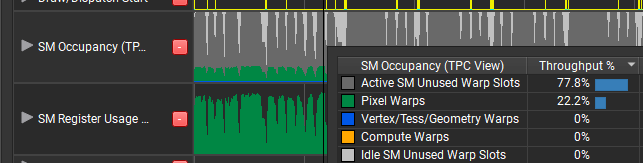
\includegraphics[width=.8\textwidth]{images/showcase/SMProfile.PNG}
    \caption{SM-Profile for a Moana Island test \ref{sec:MOANATEST} shows register and SM usage.}
    \label{fig:SMProfile}
\end{figure}
\subsection{Traversal Stack Size}
\label{sec:BottleStackSize}
AS have a weakness when it comes to geometry that contains many holes or is transparent: they lead to the traversal intersecting the PI but not intersecting the contained geometry. If there is perhaps a forest with a lot of trees of the same height and the observer is slightly above the tree line, then he intersects and traverses a substantial number of PIs that are all false positives. This leads to the issue of too small stack size. What if there are too many intersections? Then the buffer runs full, because the stack keeps growing as long as PIs are hit, which results in the traversal responding with a false negative. This occurs if there is a way to look into a number of PIs, such that the geometry inside is not intersected but the PI is. This is a significant problem and can not only be observed with the traversal shader but with only ray queries themselves, while not as significant. Therefore the question arises: How big should the traversal buffer be? Small enough to prevent register spilling but large enough so no artifacts like in \ref{fig:stackSizeLow} occur. This must be determined experimentally and on a use case basis.
\begin{figure}[h]
\subfigure[Stack runs full]{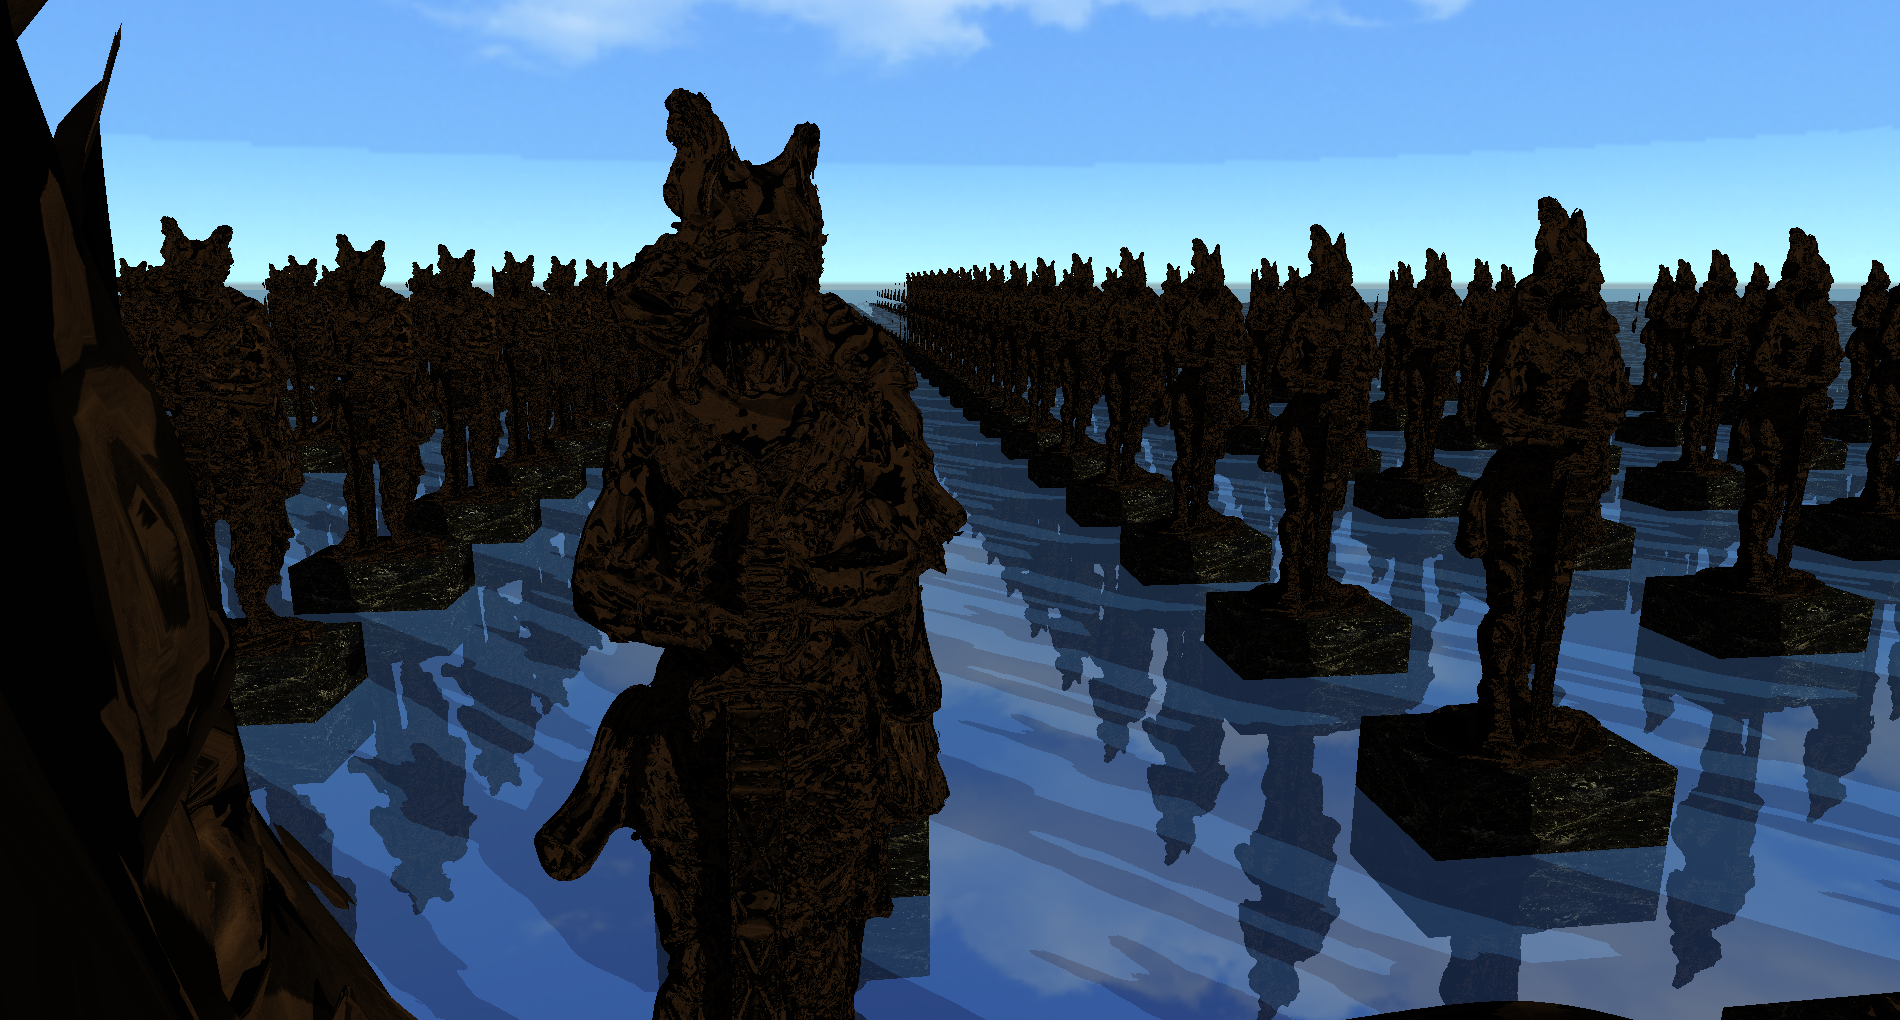
\includegraphics[width=.5\textwidth]{images/showcase/StackSizeToLow.PNG}}
\subfigure[Zoomed in view]{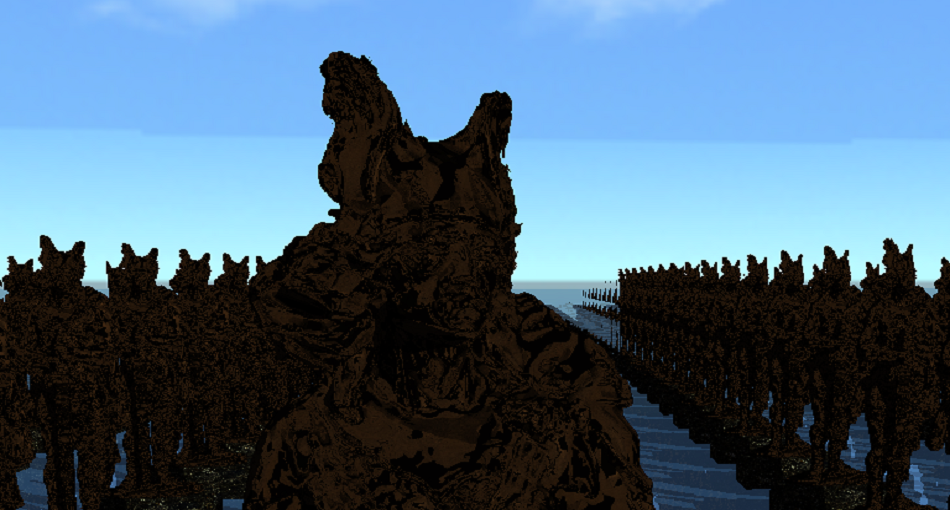
\includegraphics[width=.5\textwidth]{images/showcase/StackSizeToLowZoom.PNG}}
\caption{Ray Query for the scene intersects more PIs than the stack size allows. Size:10}
\label{fig:stackSizeLow}
\end{figure}
\subsection{Instance Overlap}
\label{sec:BottleInstanceOverlap}
AABB overlap is another problem, it occurs when the traversal hits AABB that all represent different geometry but they are tightly packed together. That way, any intersection point t in these AABBs does not necessitate a closest hit. Instead, all other geometries must also be traversed. There is no best way to resolve this issue with traversal as it stems from the scene graph and its layout itself. A possible solution would be to pack overlapping geometry into a single mesh. Therefore, the computation of a closest hit in this mesh is equivalent to a closest hit when using overlapping AABBs.\\
Another point of view is that the traversal graph can not exchange nodes and therefore cannot group overlapping geometry into the same sub-tree. Say for example two BLAS A and B contain geometry and they are to be regarded as separate geometry, but they also have a high overlap. This leads to the BLAS of A and B also overlapping, but they are not able to be merged unless they are the same mesh.
\subsection{RayQuery Speed}
\label{sec:BottleQuerySpeed}
Ray queries are fast enough to allow for up to 10-20 per pixel before any significant slowdown occurs. When using an acceleration structure with eight million instances and each having an instance of say a million triangles it is still quite fast. However, as soon as primary, shadow, reflection, and transmission rays become involved the ray queries start to reach their limit. Therefore, it is beneficial to avoid a ray query when possible.
\subsection{Shader overhead}
\label{sec:BottleShaderOverhead}
Computing an AABB intersection, multiple matrix multiplications, accessing a buffers and multiple if statements can also represent a significant slowdown. Mostly this pales in comparison to the overhead the ray queries represent. However, there are cases (ML-Instancing \ref{sec:INSTTEST}) where this becomes an issue.
\subsection{Device Limits}
\label{sec:BottleDeviceLimits}
Vulkan and by extension GPUs impose a few limitations on us. For example, a top level acceleration structure can only reference up to $2^{24}$ instances on an RTX 3060, which for our purposes might be easily surpassed. There is also buffer allocation size as well as allocation counts, GPU memory and much more. It is necessary to pay attention to these limitations, since we are trying to go as far as possible with this concept. Resulting in us exceeding these limits once the scenes start to grow larger and are no longer feasible for single-level instancing.
\newpage
\section{Shader Optimizations}
There are a couple of building blocks that can be improved. These deal with the issues described in the previous section.
\subsection{Query speed}
\label{sec:OptQuerySpeed}
To speed up the ray query as few operations as possible have to be used inside the loop. This necessitates to move the InstanceShader() function out of the while-loop. However, this function requires query values that are only obtainable as long as the PI is the current intersection candidate. Instead, the traversal payload of the parent, the custom index, primitive index and shader index offset values with the ray query candidate intersection values can be pushed onto the stack and can then let the InstanceShader run afterwards.
Then, after the RayQuery has finished, the InstanceShader function is run for all added payloads. This however complicates adding new payloads, as when adding more than one it is either necessary to move all elements to the right or to add them at the end, which in turn destroys t-Value order. This leads to the conclusion, that if the PI-Shader needs to add more than one payload, the programmable instance shader must be called from inside the while loop. This is a necessary trade off, since moving all buffer elements to the right is not very performant, especially if there are multiple instance hits, which is the common case.
\subsection{Traversal Speed}
\label{sec:OptTraversalSpeed}
\begin{figure}[b]
\hfill
\subfigure[The rendered image]{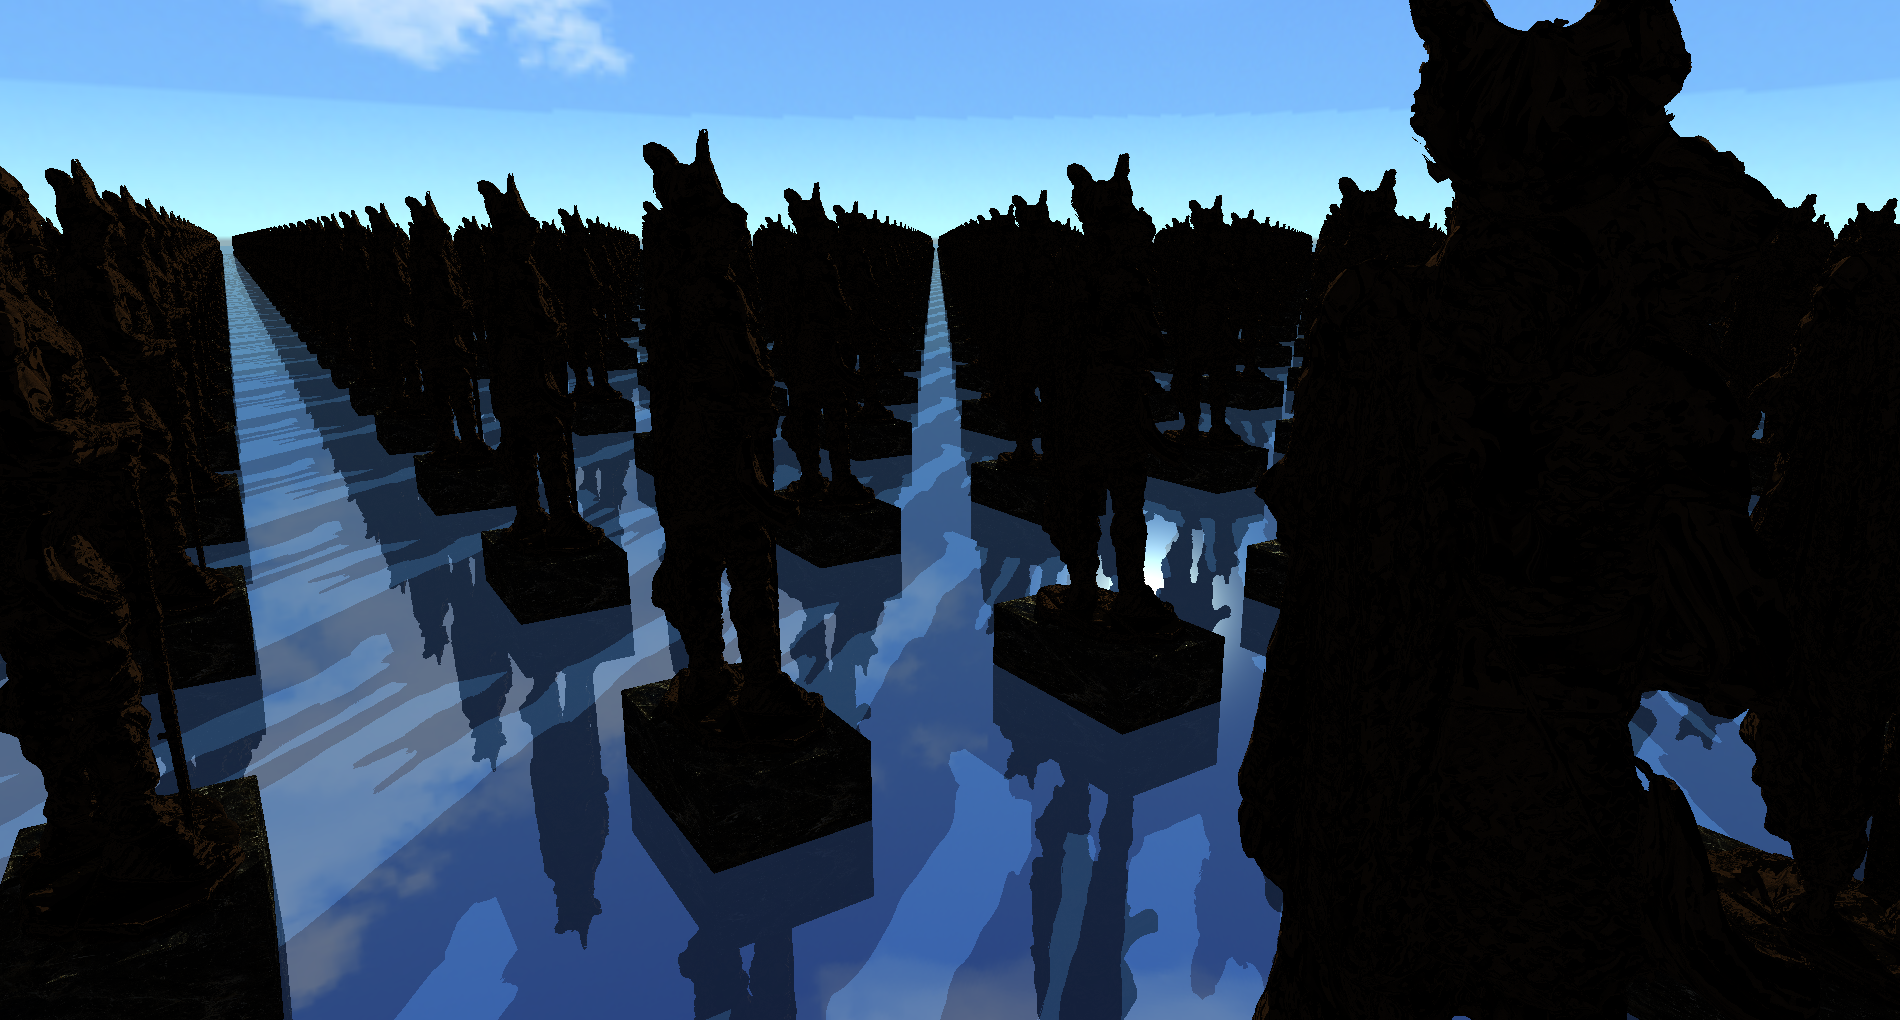
\includegraphics[width=.3\textwidth]{images/showcase/TraversalSpeedRender.PNG}}
\hfill
\subfigure[Before reversing@52FPS]{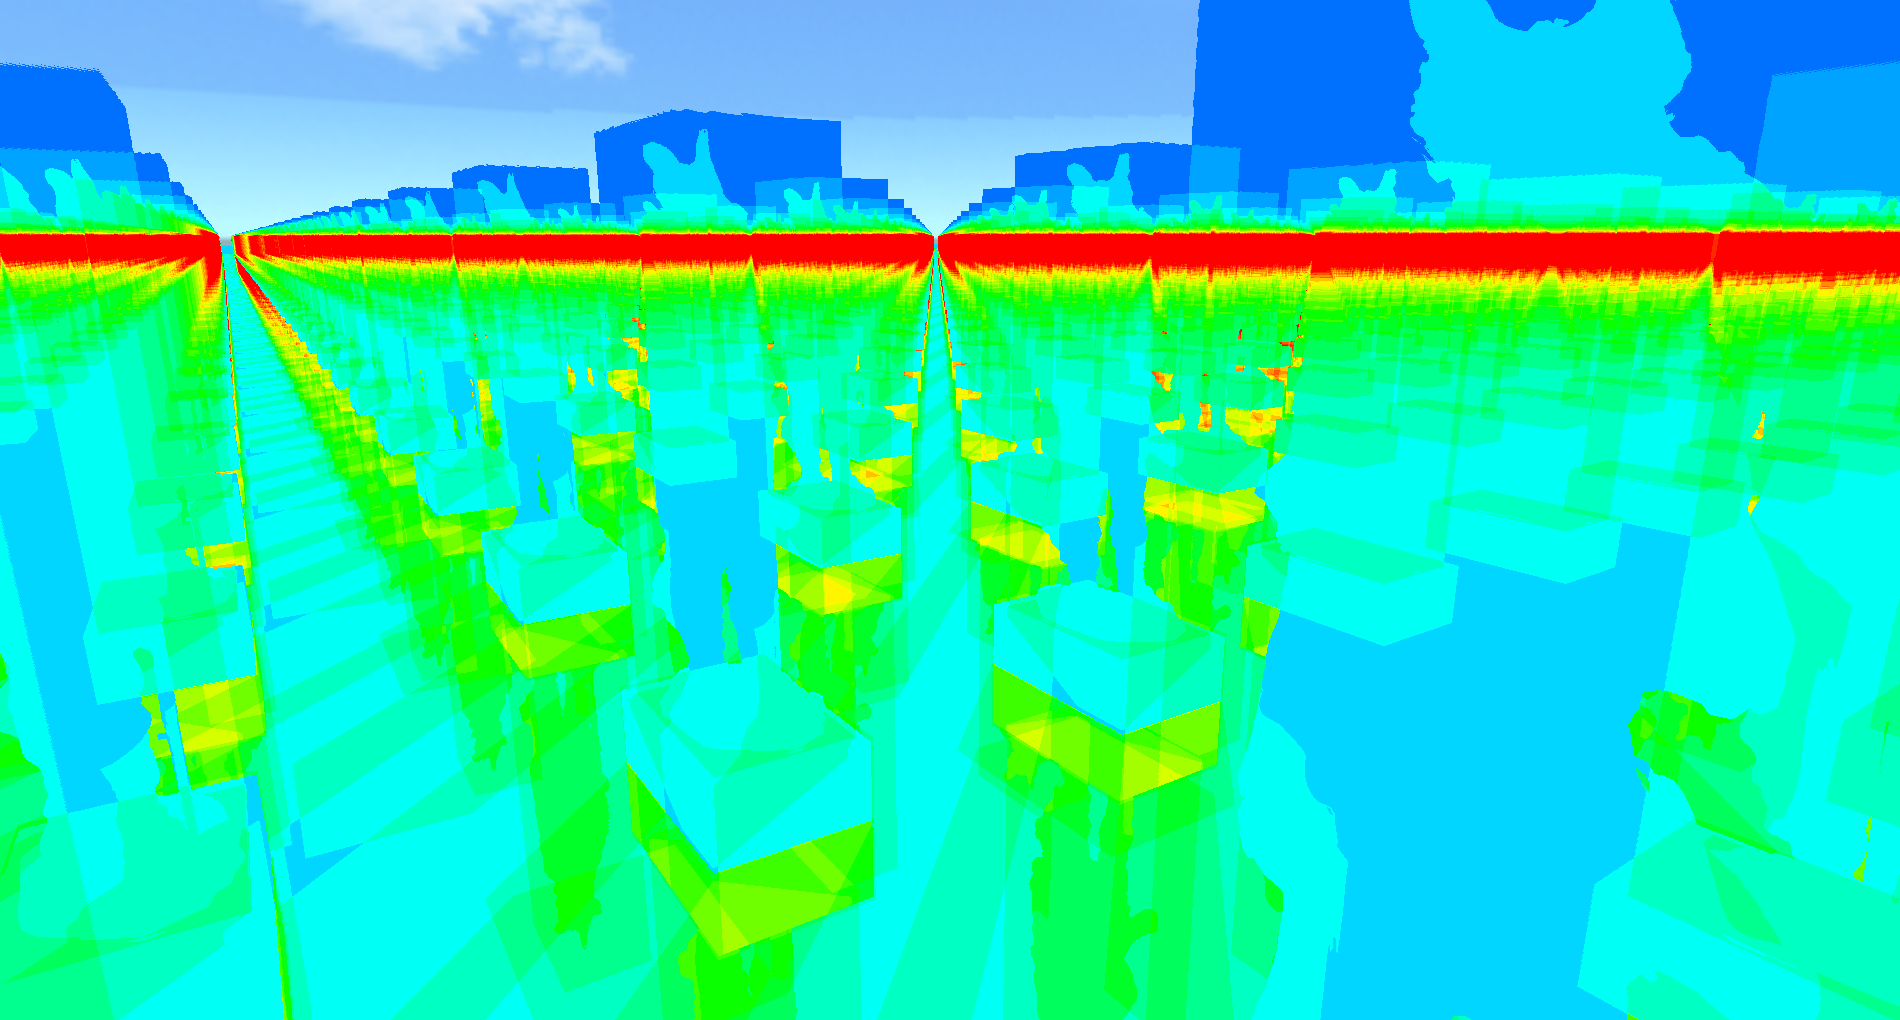
\includegraphics[width=.3\textwidth]{images/showcase/TraversalSpeedUnreveresed52FPS.PNG}}
\hfill
\subfigure[After reversing@60FPS]{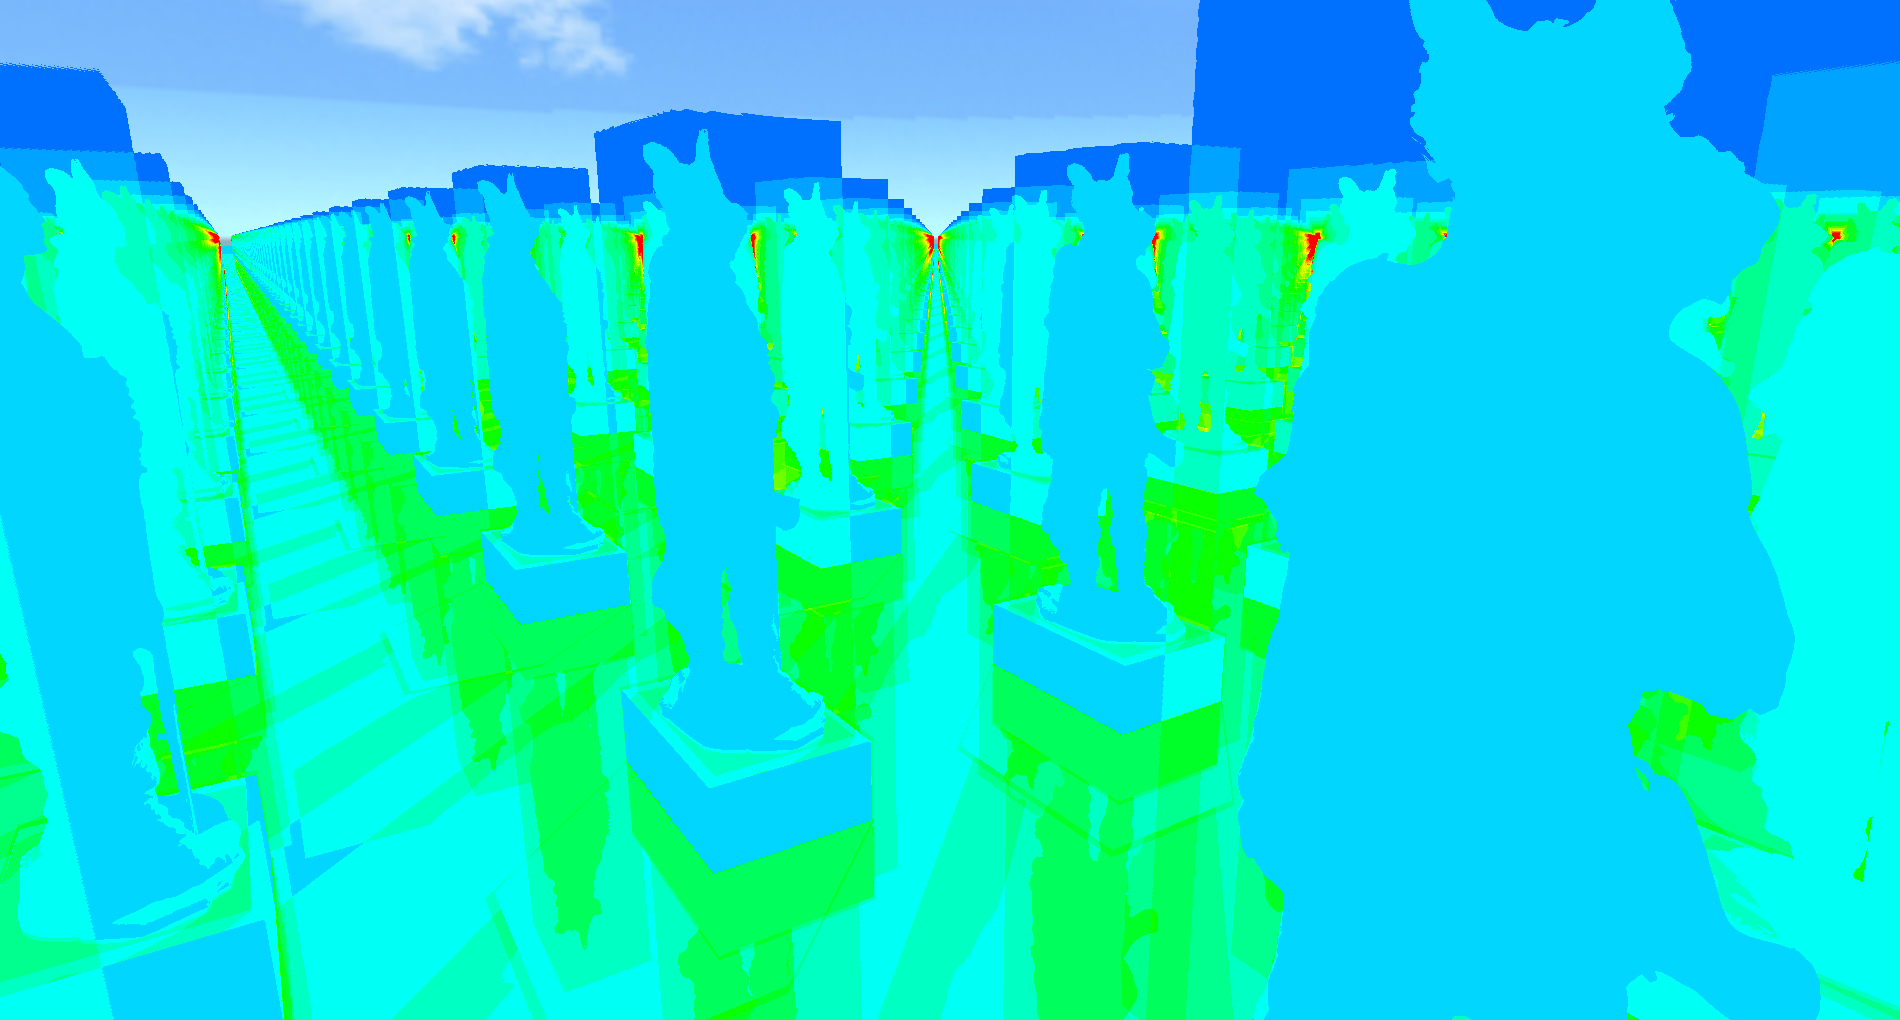
\includegraphics[width=.3\textwidth]{images/showcase/TraversalSpeedReveresed60FPS.PNG}}
\hfill
\caption{Reversing the added payloads significantly decreases query count where geometry occludes other AABBs.}
\hfill
\label{fig:TraversalSpeedQueryCount}
\end{figure}
To increase traversal speed, it is beneficial to look at the results of the ray query. The traversal tends to give low t-Values first, which leads to the conclusion that the payloads are added in ascending t-Near order. However, a fast convergence requires a depth-first search, as only on higher depths the triangles are to be found. Additionally, when using a breath first approach, the traversal buffer size will keep expanding massively with every level. So, the goal is to find better values for best\_t as fast as possible.\\
To do this, the first step is reversing the added traversal loads after the query has finished, so that the last element is the one with about the lowest t-Near value. This leads to the algorithm most likely choosing an AABB with a t-Value that is as low as can be. Next, the DFS chooses that payload to continue traversal first. If there then happens to be a triangle intersection, we then have a good lower bound for the traversal. This makes it possible to skip quite a lot of payloads that have a t-Near value worse than best\_T. The improvement in query count can be seen in \ref{fig:TraversalSpeedQueryCount}\\
Note:\\
In testing, I found that Vulkan does not guarantee for ascending t-Values for intersected AABBs. I noticed the strange behavior that for positive t-Near values the order of intersections is strictly increasing, but once negative t-Near values become involved, i.e. the query is started from inside the AABB, they can be intersected quite late, which, if the traversal Stack size is too low can lead to artifacts.

\subsection{Traversal Buffer Size}
\label{sec:OptStackMemorySize}
One big question was how to represent the transform of the ray in the traversal stack. The first approach was using two Vec3 to save origin and direction of the transformed ray. However, it quickly became apparent that this was not a suitable solution. This is due to the issue of transforming surface normals from object to world space. I the end, this made it necessary to keep a full transform of scale, rotation, and translation to properly transform all necessary values into their respective coordinate systems. Next comes the question of how to represent this transform.\\
The final layout is using a mat4x3, in question were also quaternions, but since a Vec3 is 16 byte aligned in the end it did not make a difference regarding traversal buffer size. Instead, it was better to opt for fewer operations. To improve ray query speed, it is also required to keep track of t-Values and ray query intersection candidate values\ref{sec:OptQuerySpeed}. A payload then requires 64bytes and looks like this:
\begin{lstlisting}
struct TraversalPayload {
	mat4x3 world_to_object;
	float tNear;  // the t for which this aabb was intersected
	int cIdx_nIdx;// after compute: node index
	              // before compute: custom index
	int pIdx_lod; // after compute: LOD
	              // before compute: primitive index
	int sIdx_un;  // after compute: unsused
	              // before compute: shaderOffset (grandchild)
};
\end{lstlisting}
Notice that the three int fields have different uses depending on if the InstanceShader() function was already called for this payload \ref{sec:OptTraversalSpeed}.\\
Thus, with less memory usage it is possible to increase the stack size, which in turn can deal with the problem of a to small stack size in \ref{sec:BottleStackSize}. However, the amount of queries in \ref{fig:stackSizeHigh} is far too much. A way to prevent this is not to use the traversal shader to handle multiple instance hits. Instead, the ray query handles these types of instances, since it is solved by the fixed function ray traversal. This will be talked about next.
\begin{figure}
\subfigure[Correctly rendered figures]{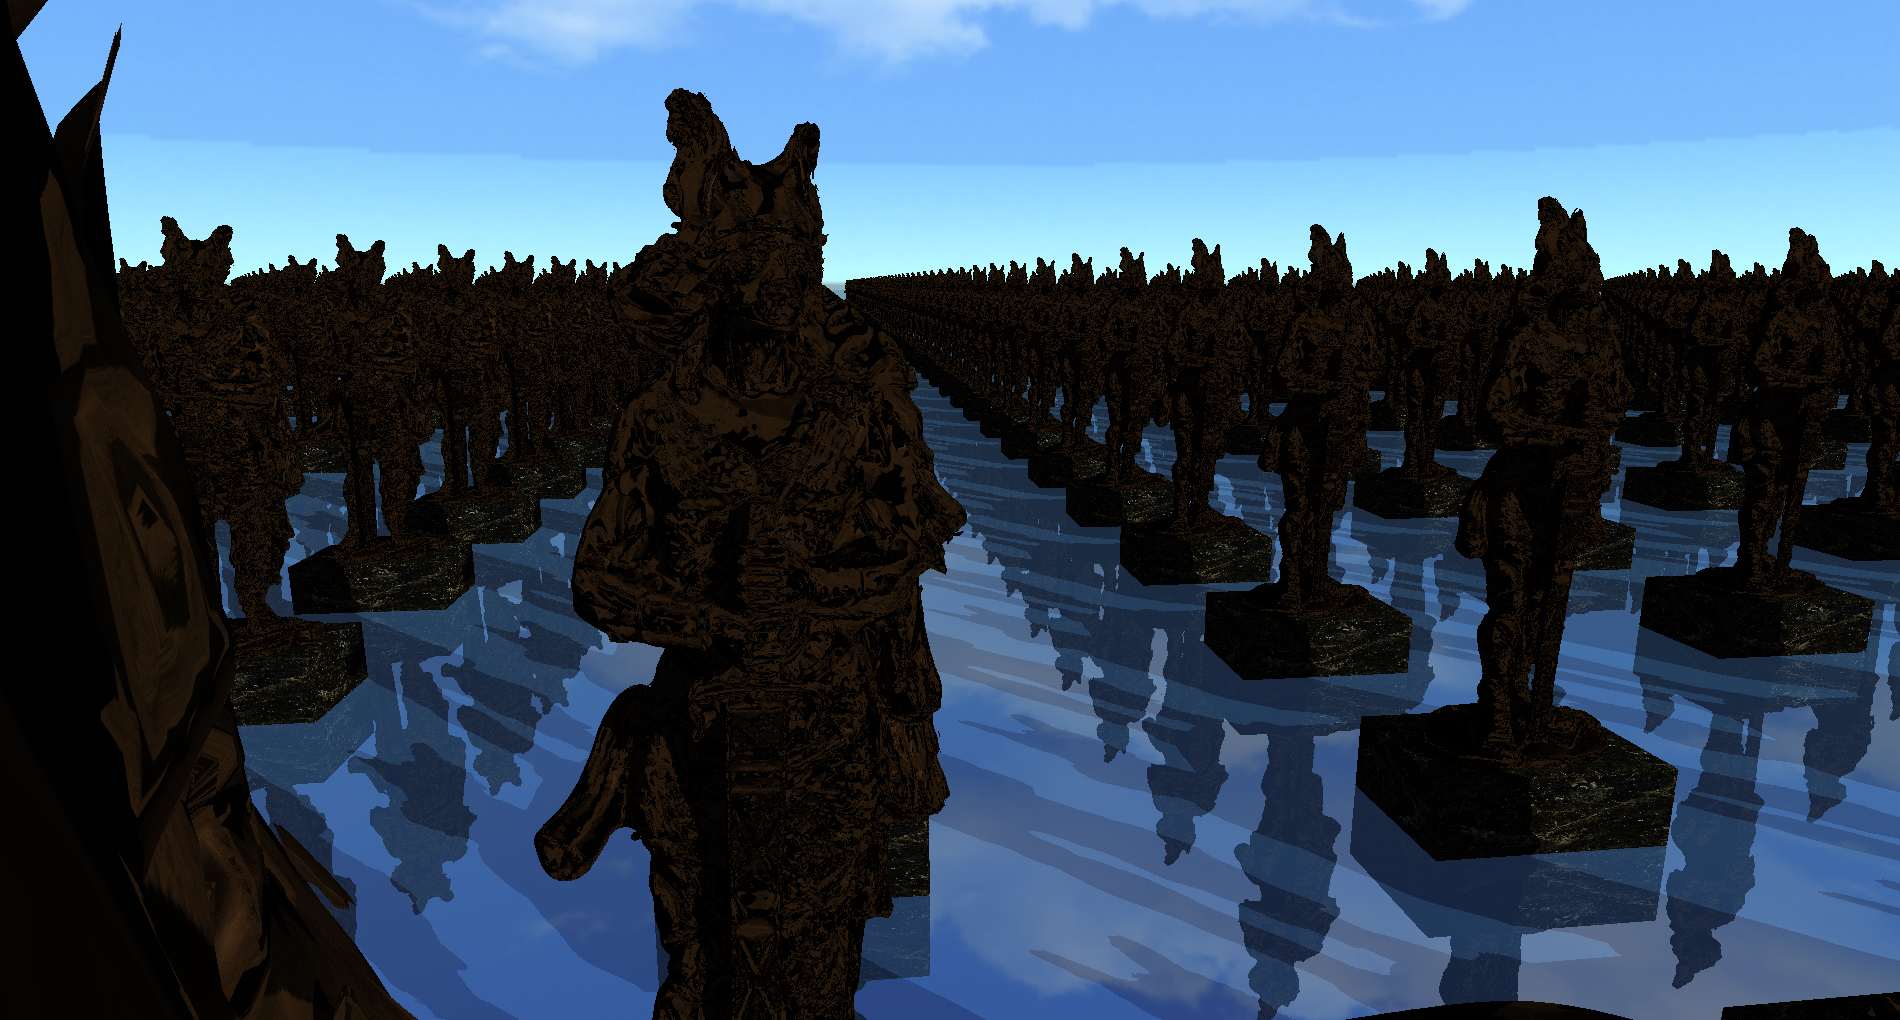
\includegraphics[width=.5\textwidth]{images/showcase/StackSizeLargeEnough.PNG}}
\subfigure[Ray query count per pixel]{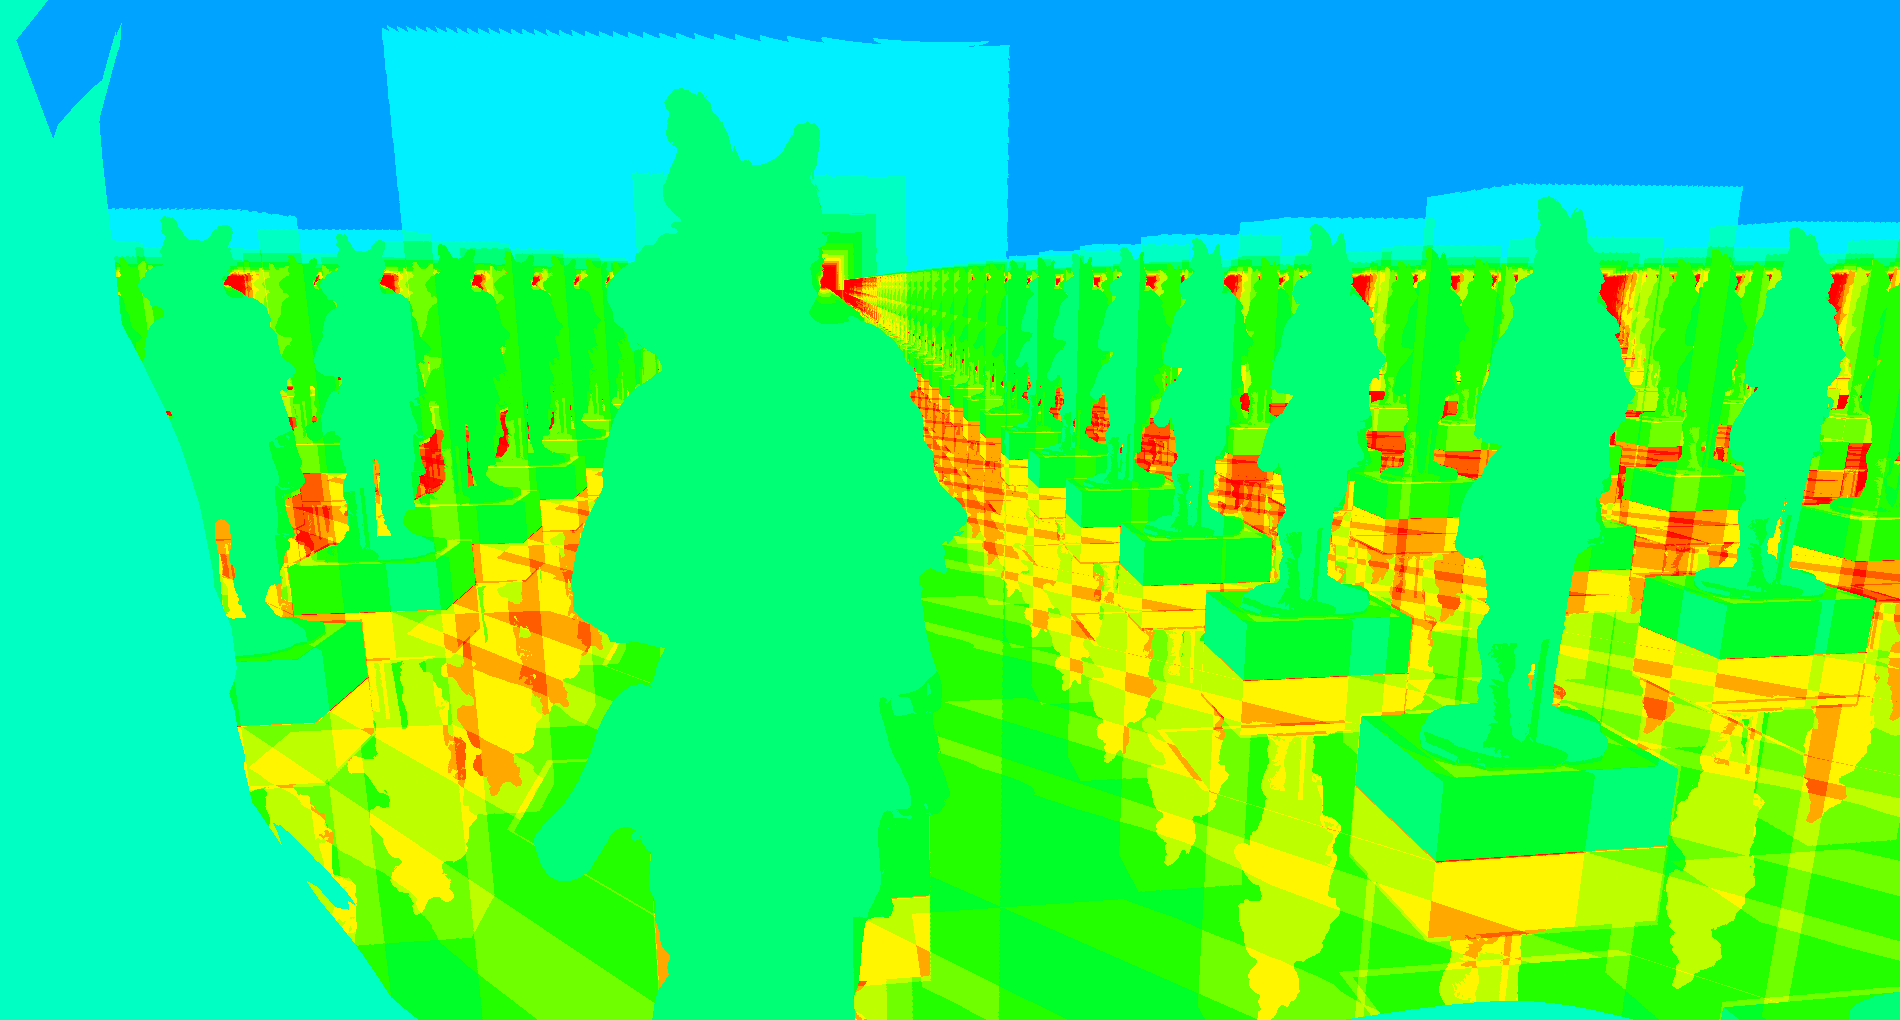
\includegraphics[width=.5\textwidth]{images/showcase/StackSizeQueryCount.PNG}}
\caption{Other than in \ref{fig:stackSizeLow} the stack size is now large enough to prevent the artifacts.}
\label{fig:stackSizeHigh}
\end{figure}

\newpage
\subsection{Traversal stack size}
\label{sec:OptStackSize}

\begin{figure}
    \centering
    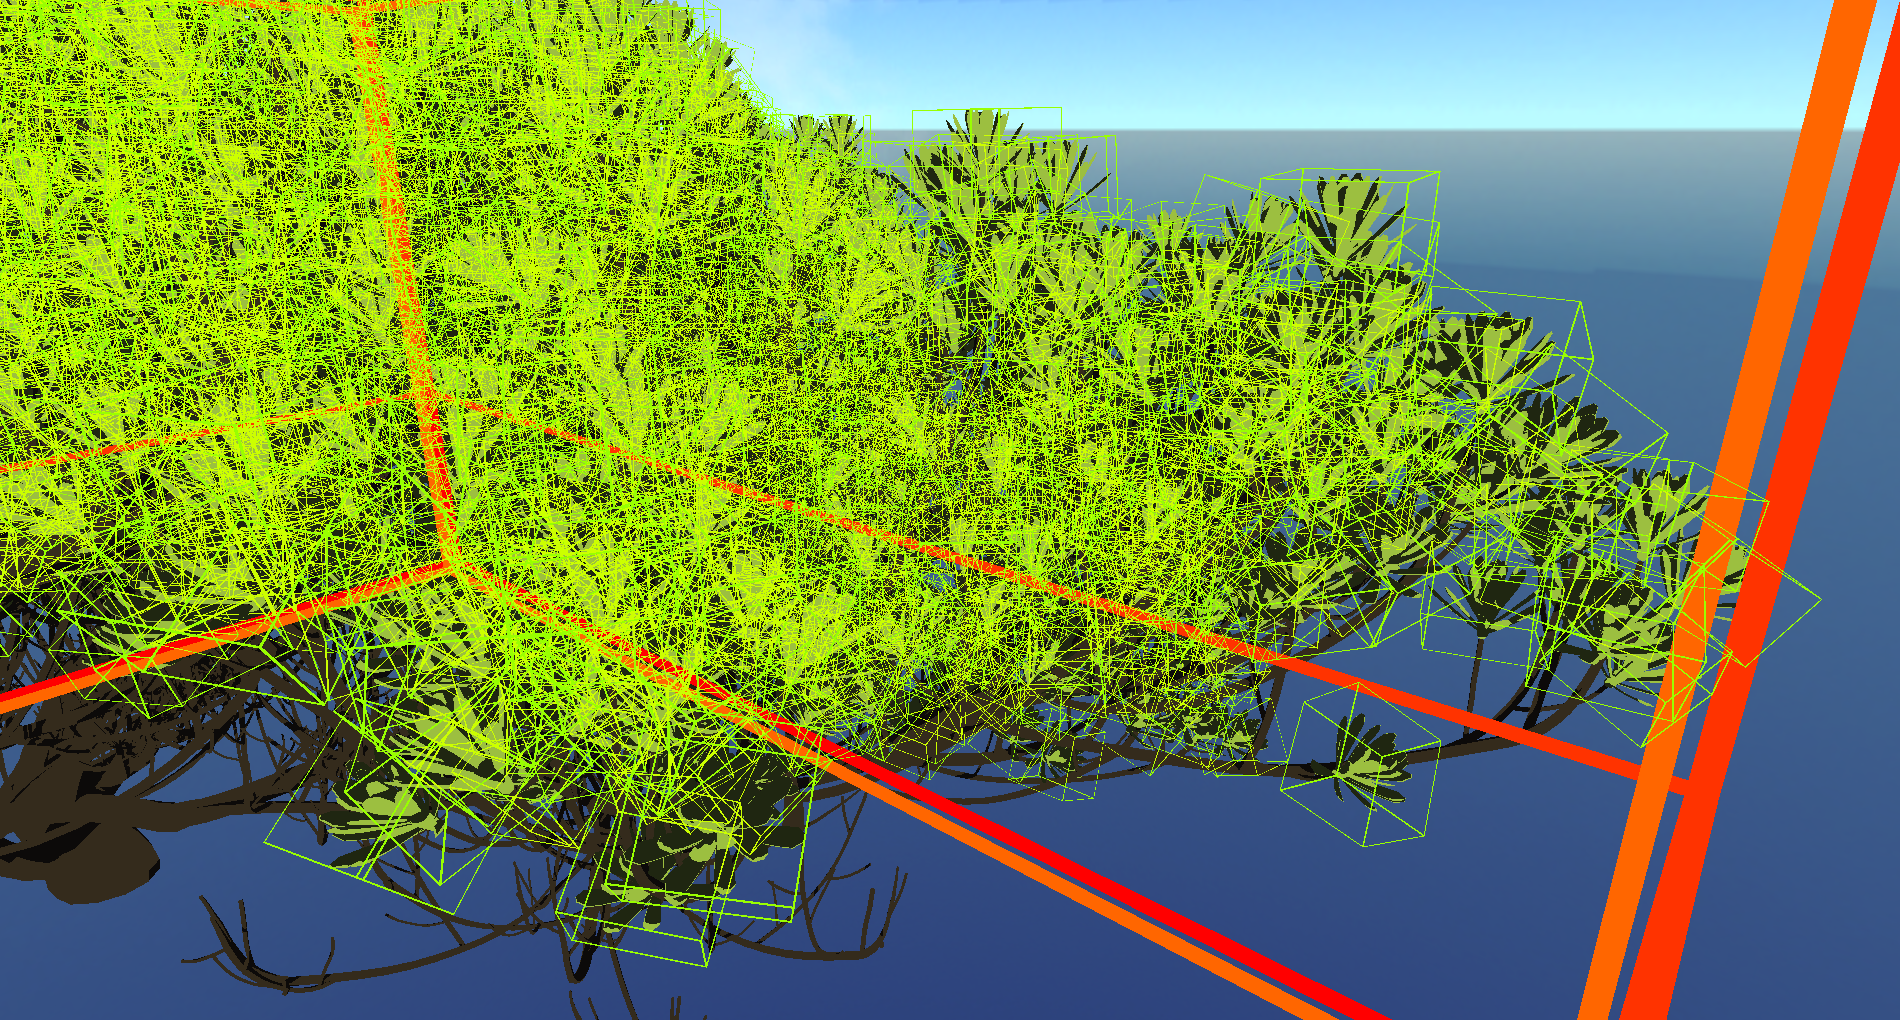
\includegraphics[width=.8\textwidth]{images/showcase/ManyAABBs.PNG}
    \caption{Too many PIs.}
    \label{fig:manyAABBs}
\end{figure}

\begin{figure}
    \centering
    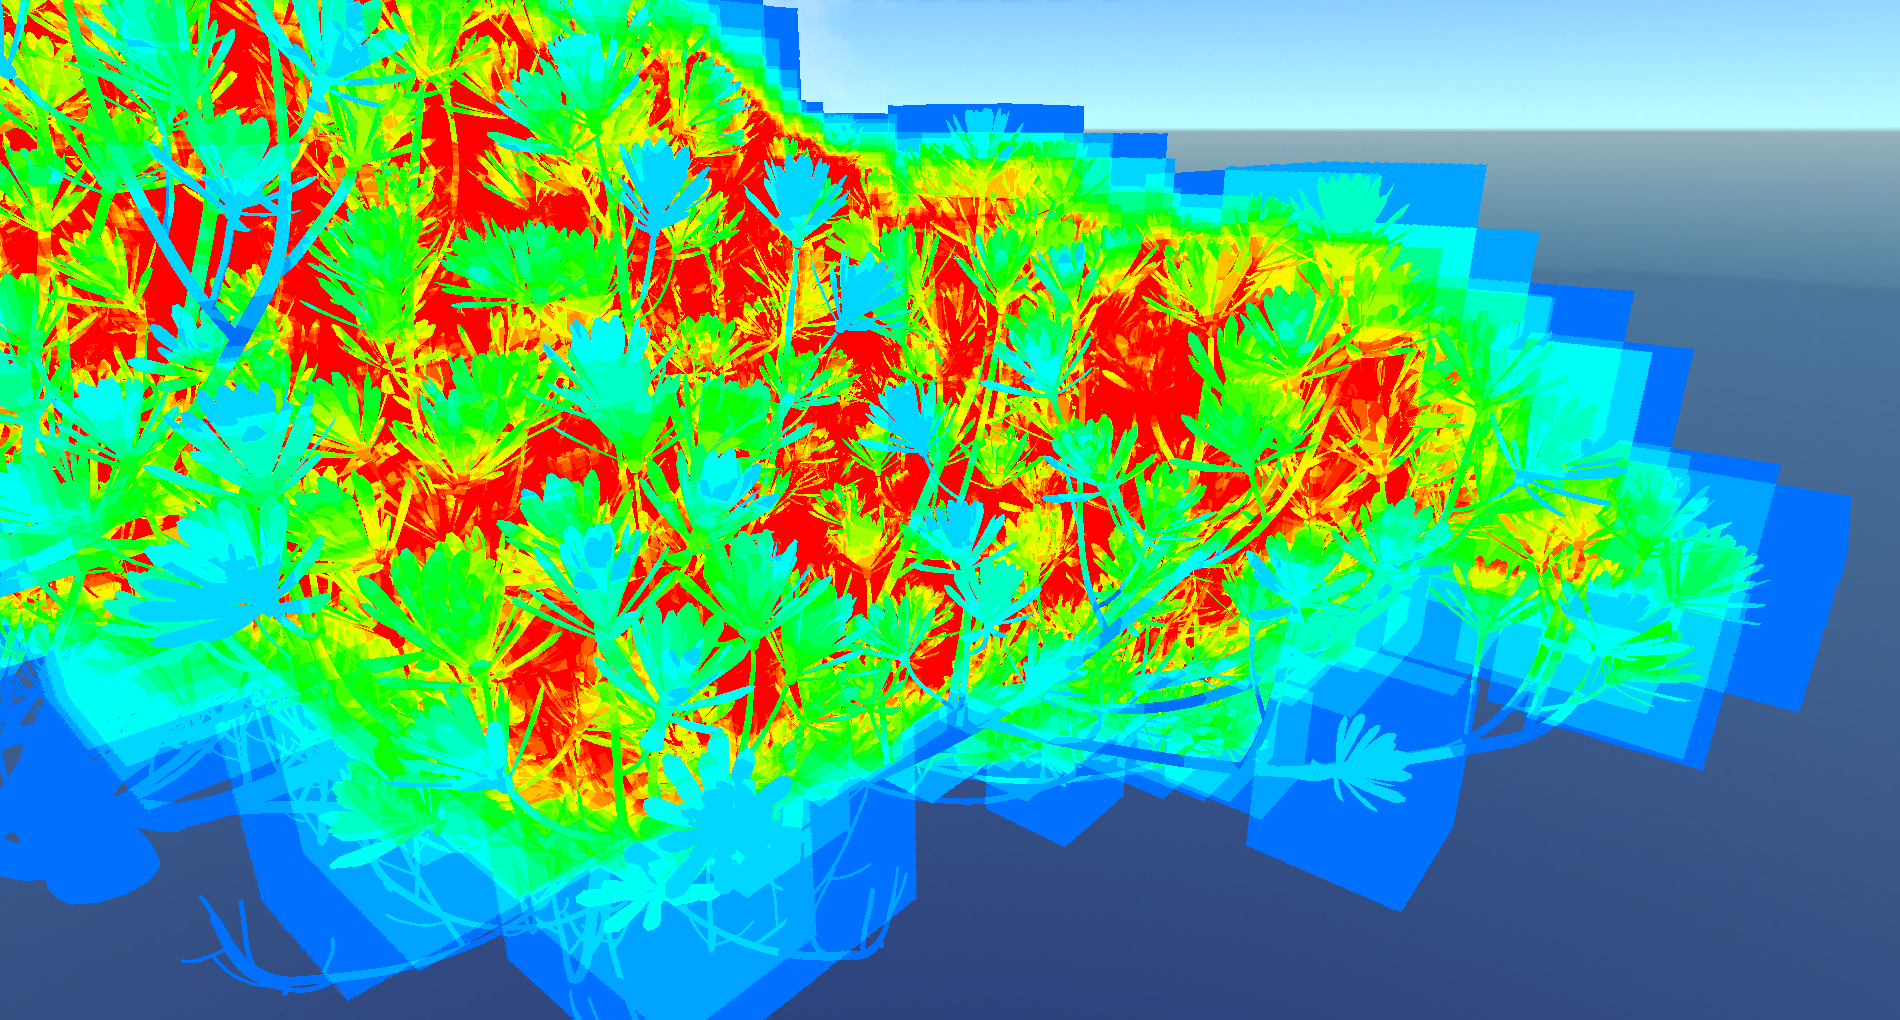
\includegraphics[width=.8\textwidth]{images/showcase/ManyAABBsQuery24FPS.PNG}
    \caption{Ray Query count slows application down to 24FPS.}
    \label{fig:manyAABBQueryCount}
\end{figure}
Currently there is the method to construct an acceleration structure for every single node. This is, to put it mildly, highly inefficient. A better way to do it is to flag a node that its children are only to be regarded as transforms to lower nodes. We will call this type of node InstanceList. The first time this occurred was when dealing with a high instance intersection count. What happened is that many AABBs were the leaves of a tree and the traversal proceeded to add all leafs to the payload stack. This in turn lead to many invocations of the InstanceShader(), because the tree was represented by an even node with a TLAS. This node had an odd child that represented the tree geometry and about 8000 odd children for the leaves. These, in turn, referenced another even node that contained the geometry (another TLAS). This resulted in an  InstanceShader() invocation for each added payload, which easily was about 70-80 in some cases. See \ref{fig:manyAABBs} and \ref{fig:manyAABBQueryCount}.\\
This brings us back to the principle: Only call the InstanceShader() when it is necessary! In this case it is not. It is just a list of instances inside an acceleration structure. The solution to this is to incorporate the transforms into the TLAS instead and to only regard them as transforms to the BLAS which contained the leaf geometry. Resulting in the traversal to instead invoke the InstanceShader not a single time instead of 60-80 times. See \ref{fig:instanceListAABB} and \ref{fig:instanceListQueryCount}\\
It is also possible to introduce the same principle for odd nodes. Flag them as InstanceLists, and to regard all their children only as transforms. There is a small constraint here though: An instance an odd node must reference exactly one child. This is due to the fact that there is no way to properly retrieve the intersected instance with the given ray query index functions \ref{sec:VkRayQuery}, unless the shader should add all intersected children. However, when using InstanceLists on an odd level with more than one children leads to the problem with adding more than one payload \ref{sec:OptQuerySpeed}.
\begin{figure}
    \centering
    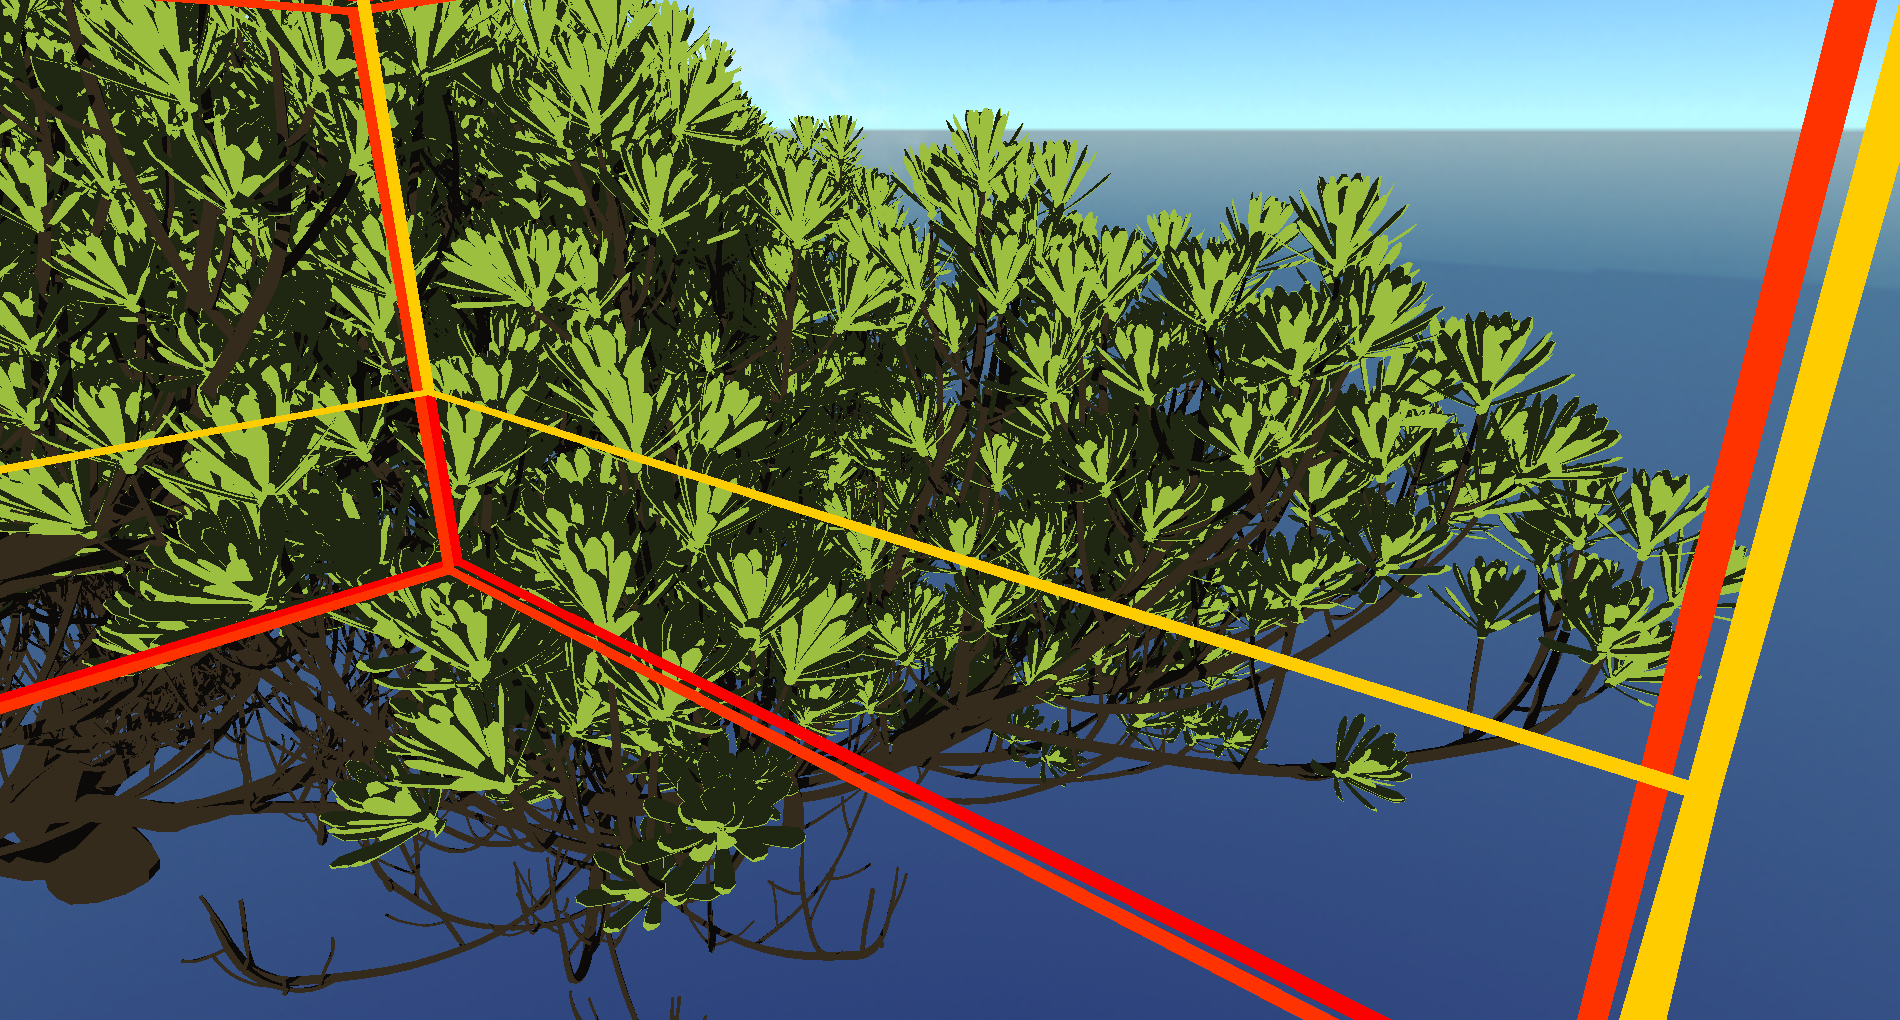
\includegraphics[width=.8\textwidth]{images/showcase/InstanceListAABB.PNG}
    \caption{The PIs are merged into the higher level.}
    \label{fig:instanceListAABB}
\end{figure}

\begin{figure}
    \centering
    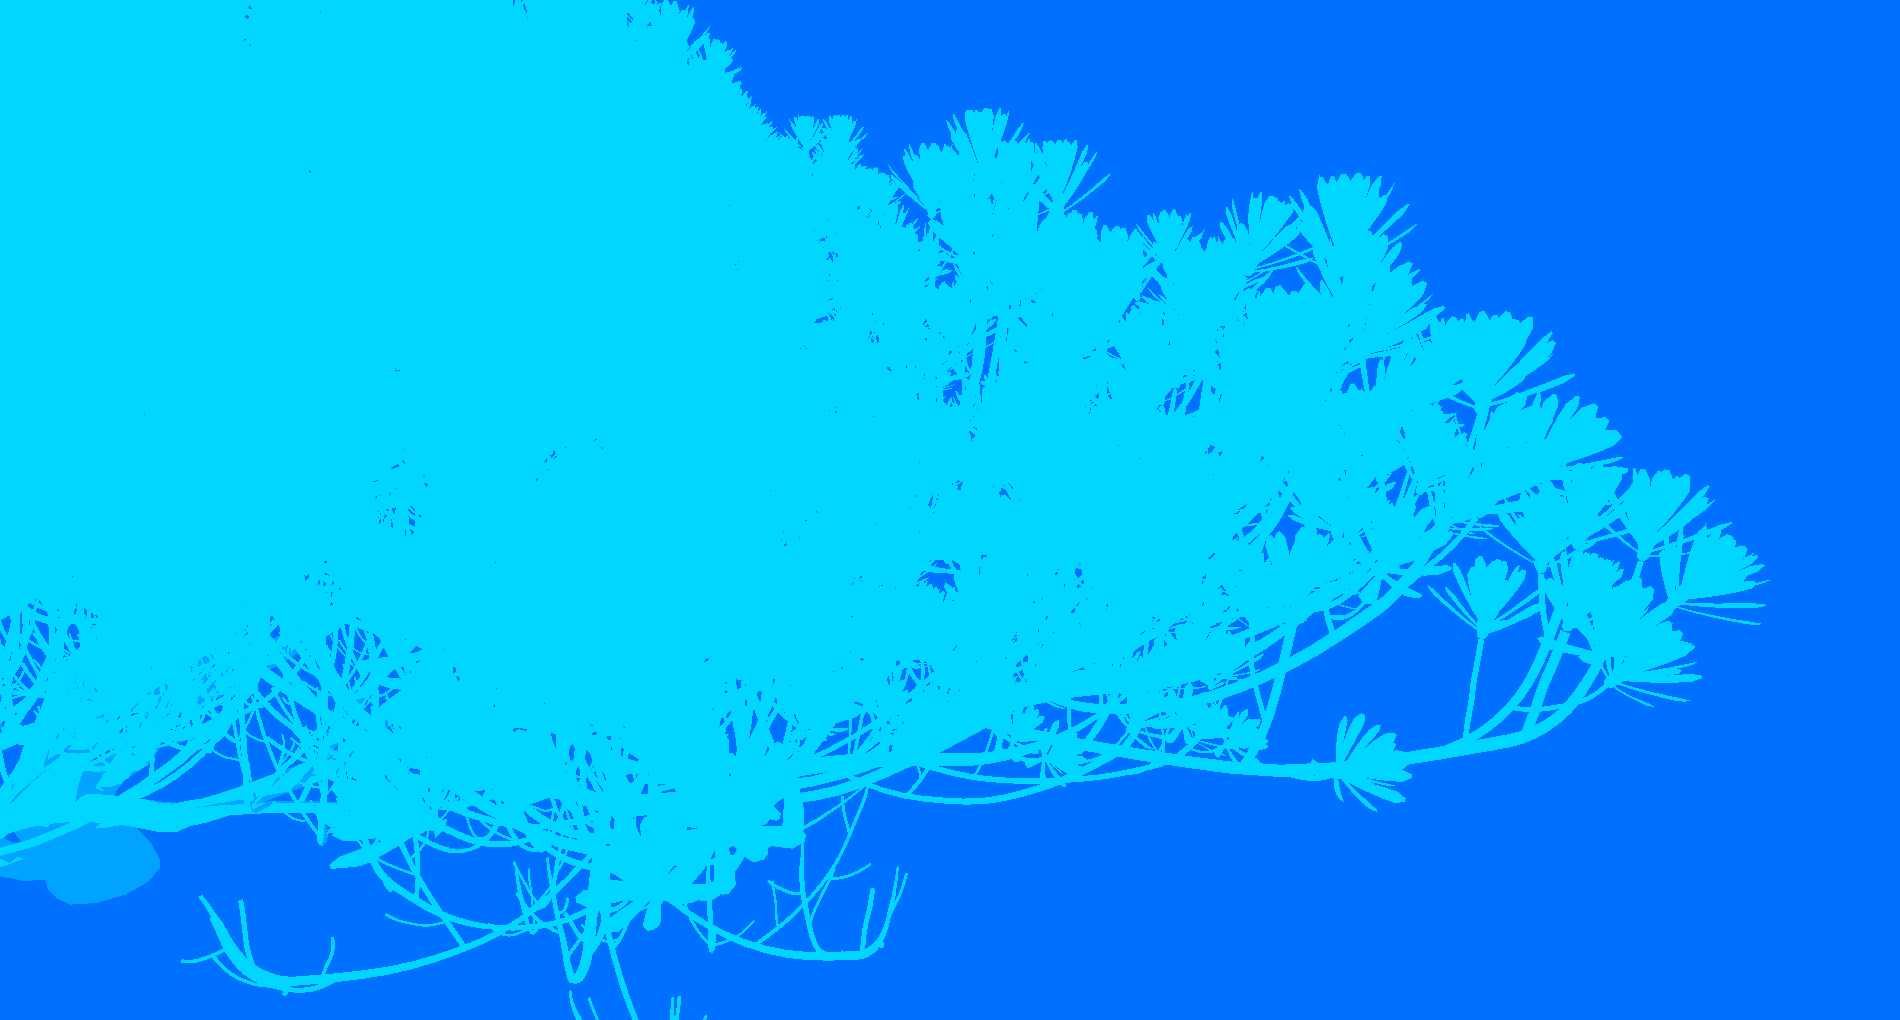
\includegraphics[width=.8\textwidth]{images/showcase/InstanceListAABBQuery220FPS.PNG}
    \caption{Ray Query count decreases and now runs at 220FPS instead of 24FPS.}
    \label{fig:instanceListQueryCount}
\end{figure}

\newpage
\subsection{AABB Overlap}
\label{sec:OptInstanceOverlap}

\begin{figure}
    \hfill
    \subfigure[Unmerged AABBs]{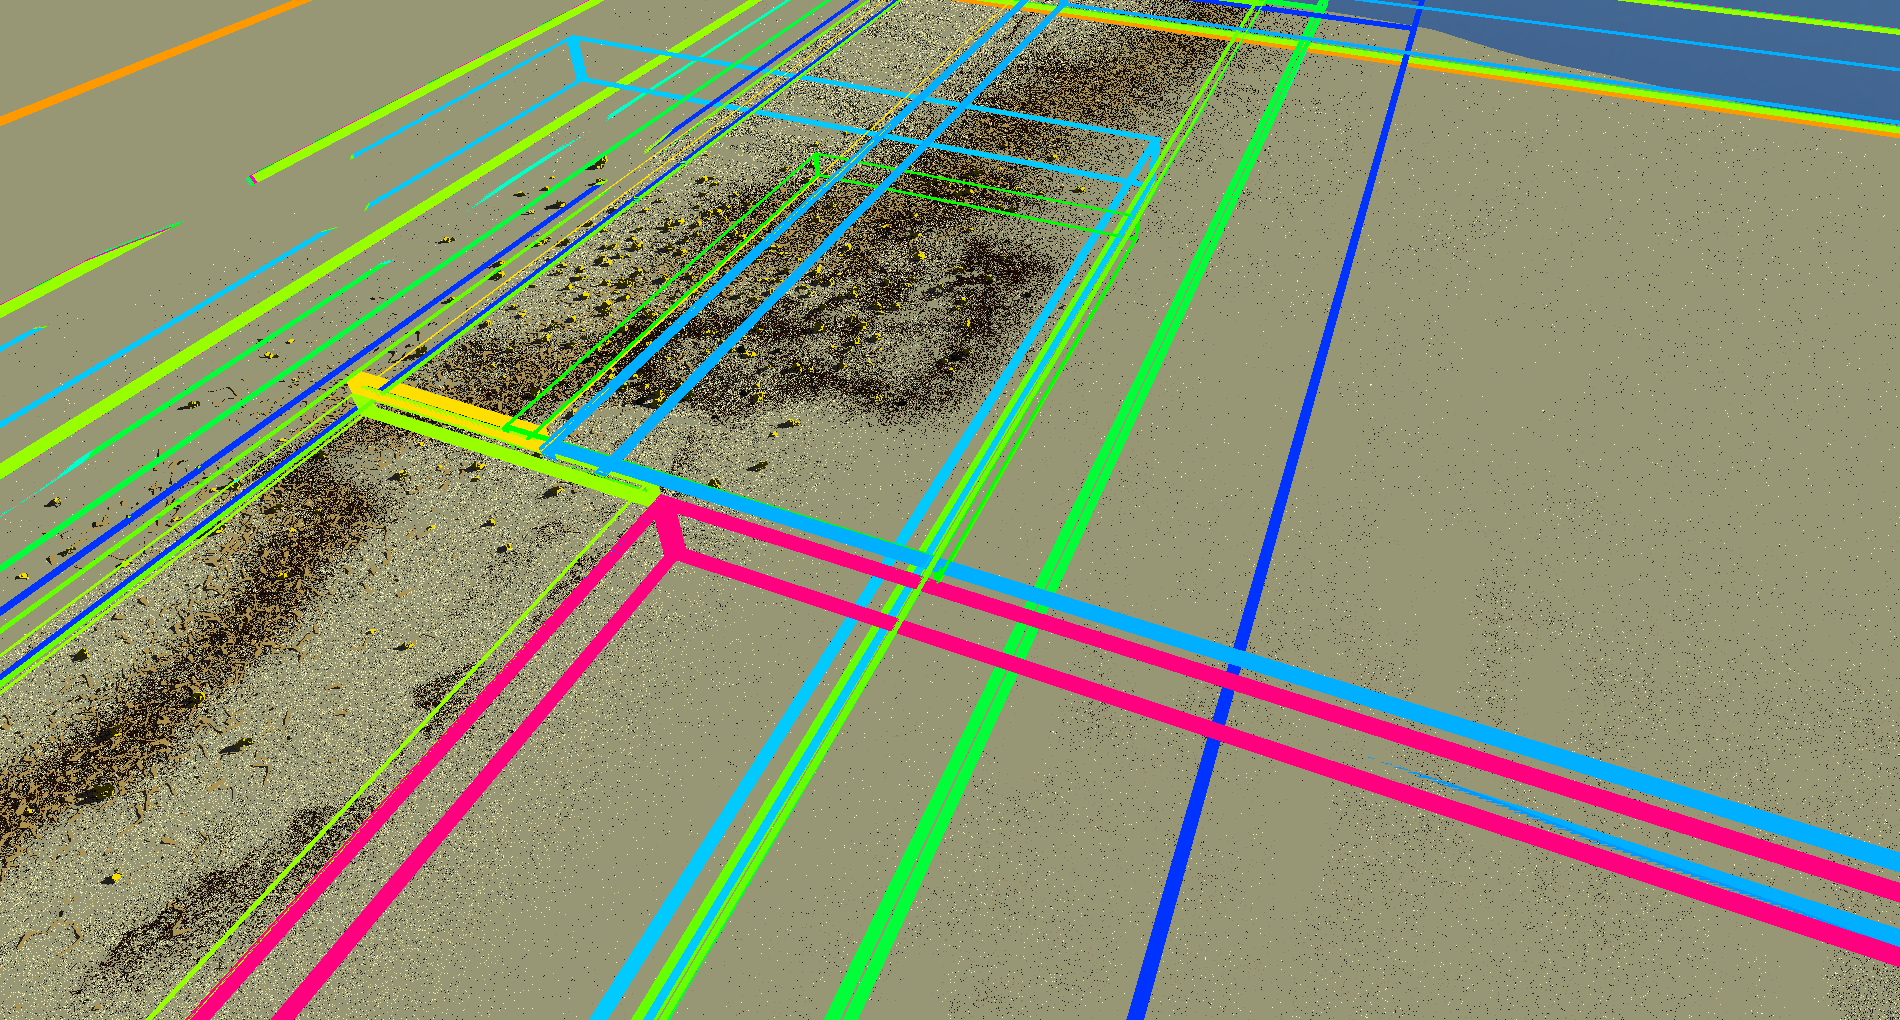
\includegraphics[width=.45\textwidth]{images/showcase/BeachUnmerged.PNG}}
    \hfill
    \subfigure[Ray query count]{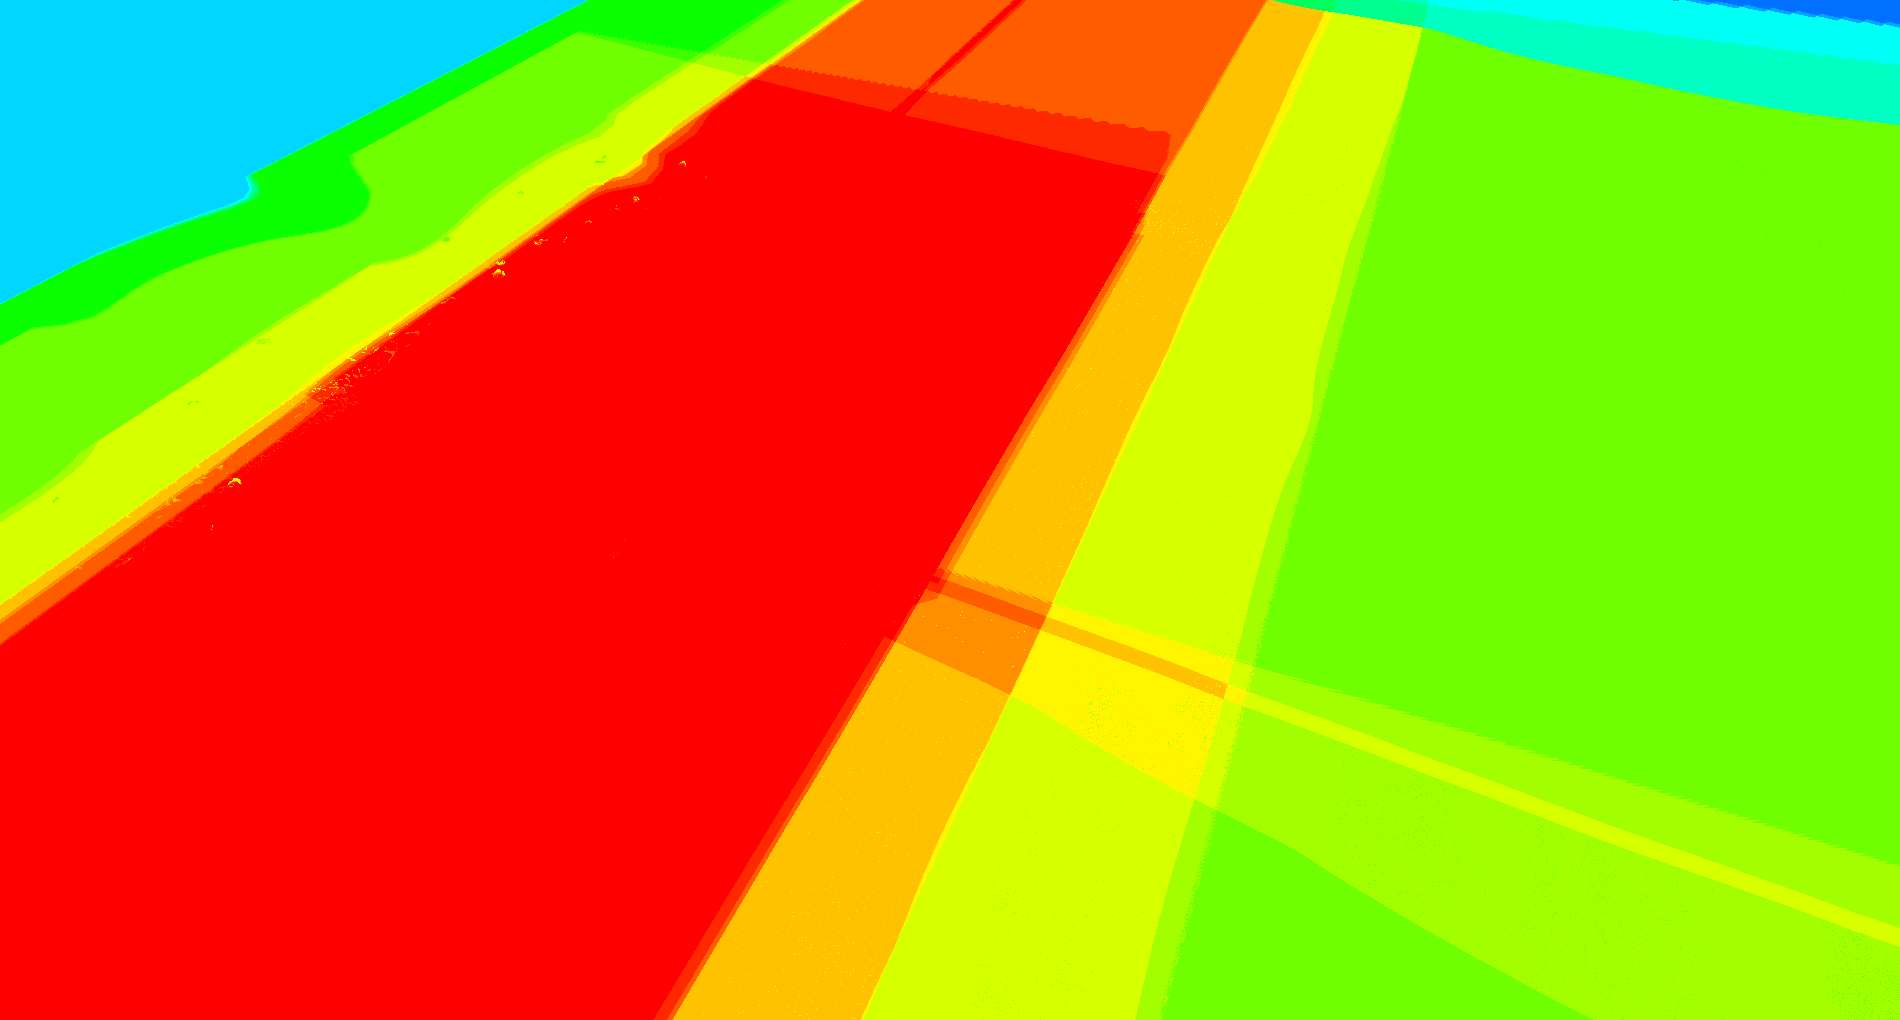
\includegraphics[width=.45\textwidth]{images/showcase/BeachUnmergedQuery38FPS.PNG}}
    \hfill
    \caption{Overlapping AABBs cause an increase in ray queries. Running @38FPS.}
    \label{fig:beachUnmerged}
\end{figure}

\begin{figure}
    \hfill
    \subfigure[Reorganized AABBs]{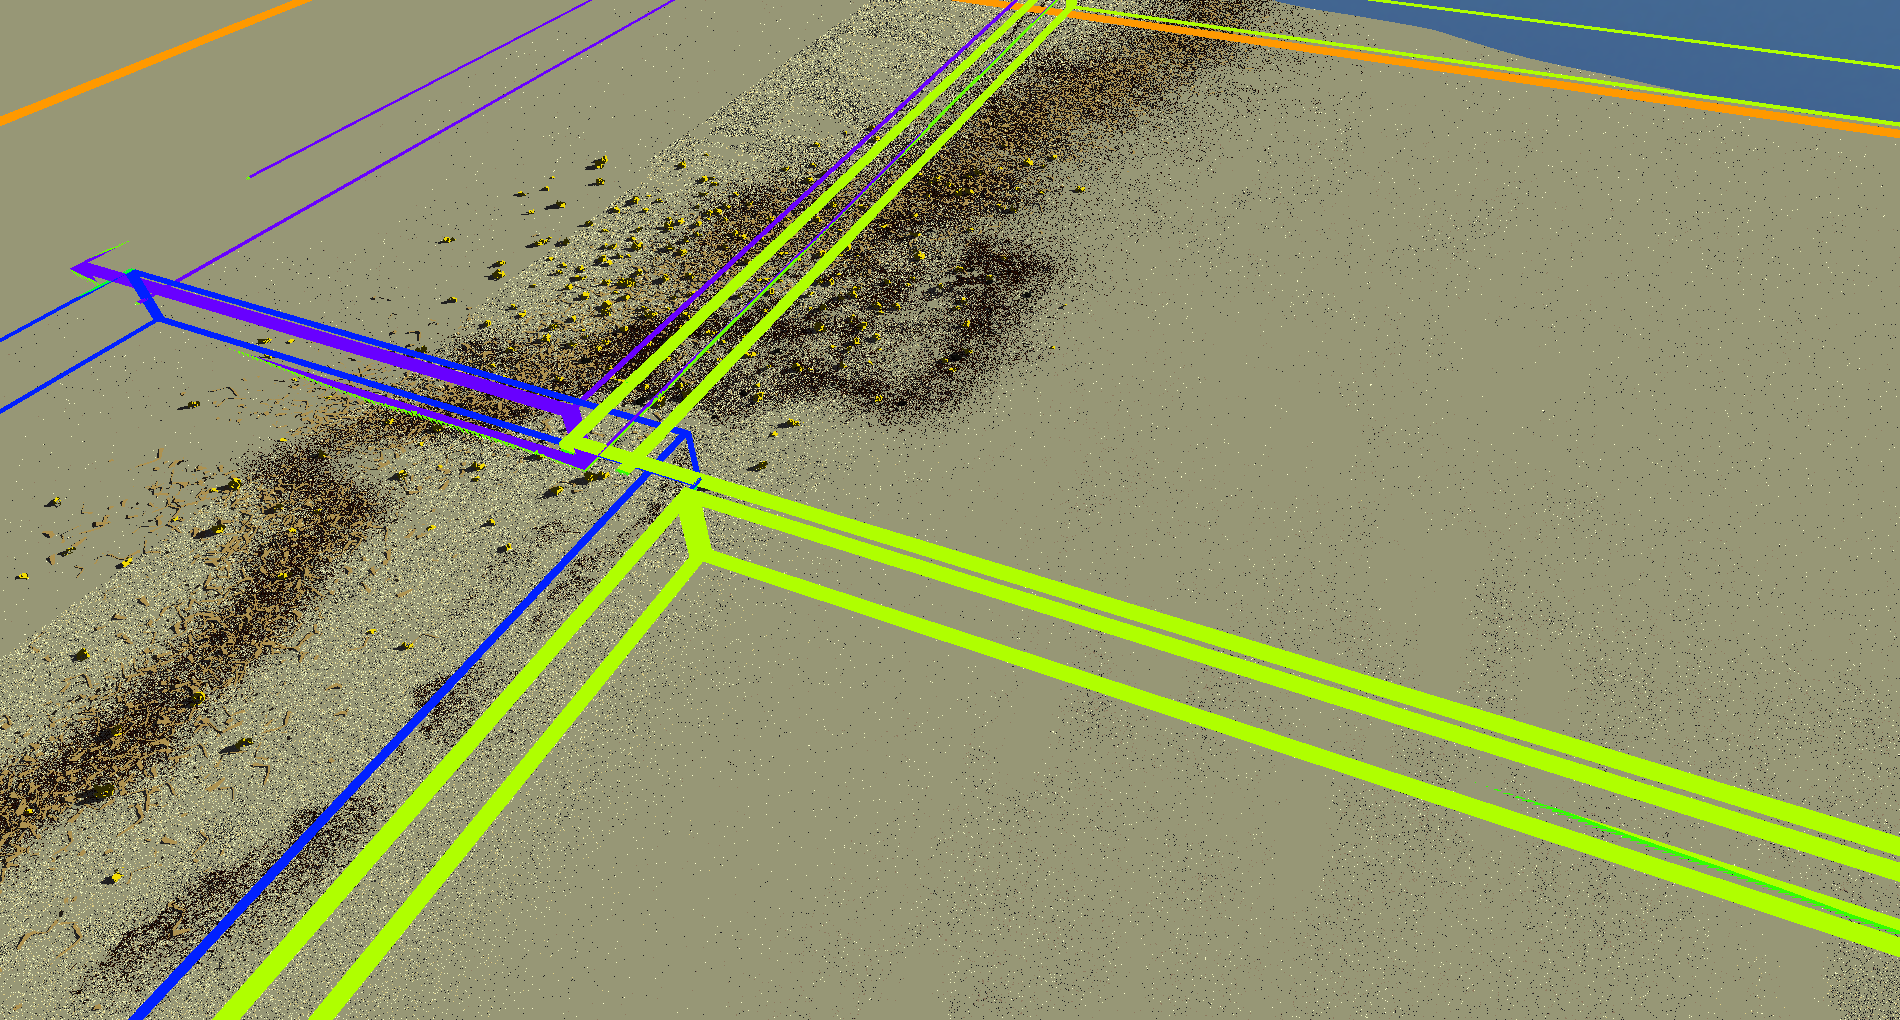
\includegraphics[width=.45\textwidth]{images/showcase/BeachMerged.PNG}}
    \hfill
    \subfigure[Ray query count]{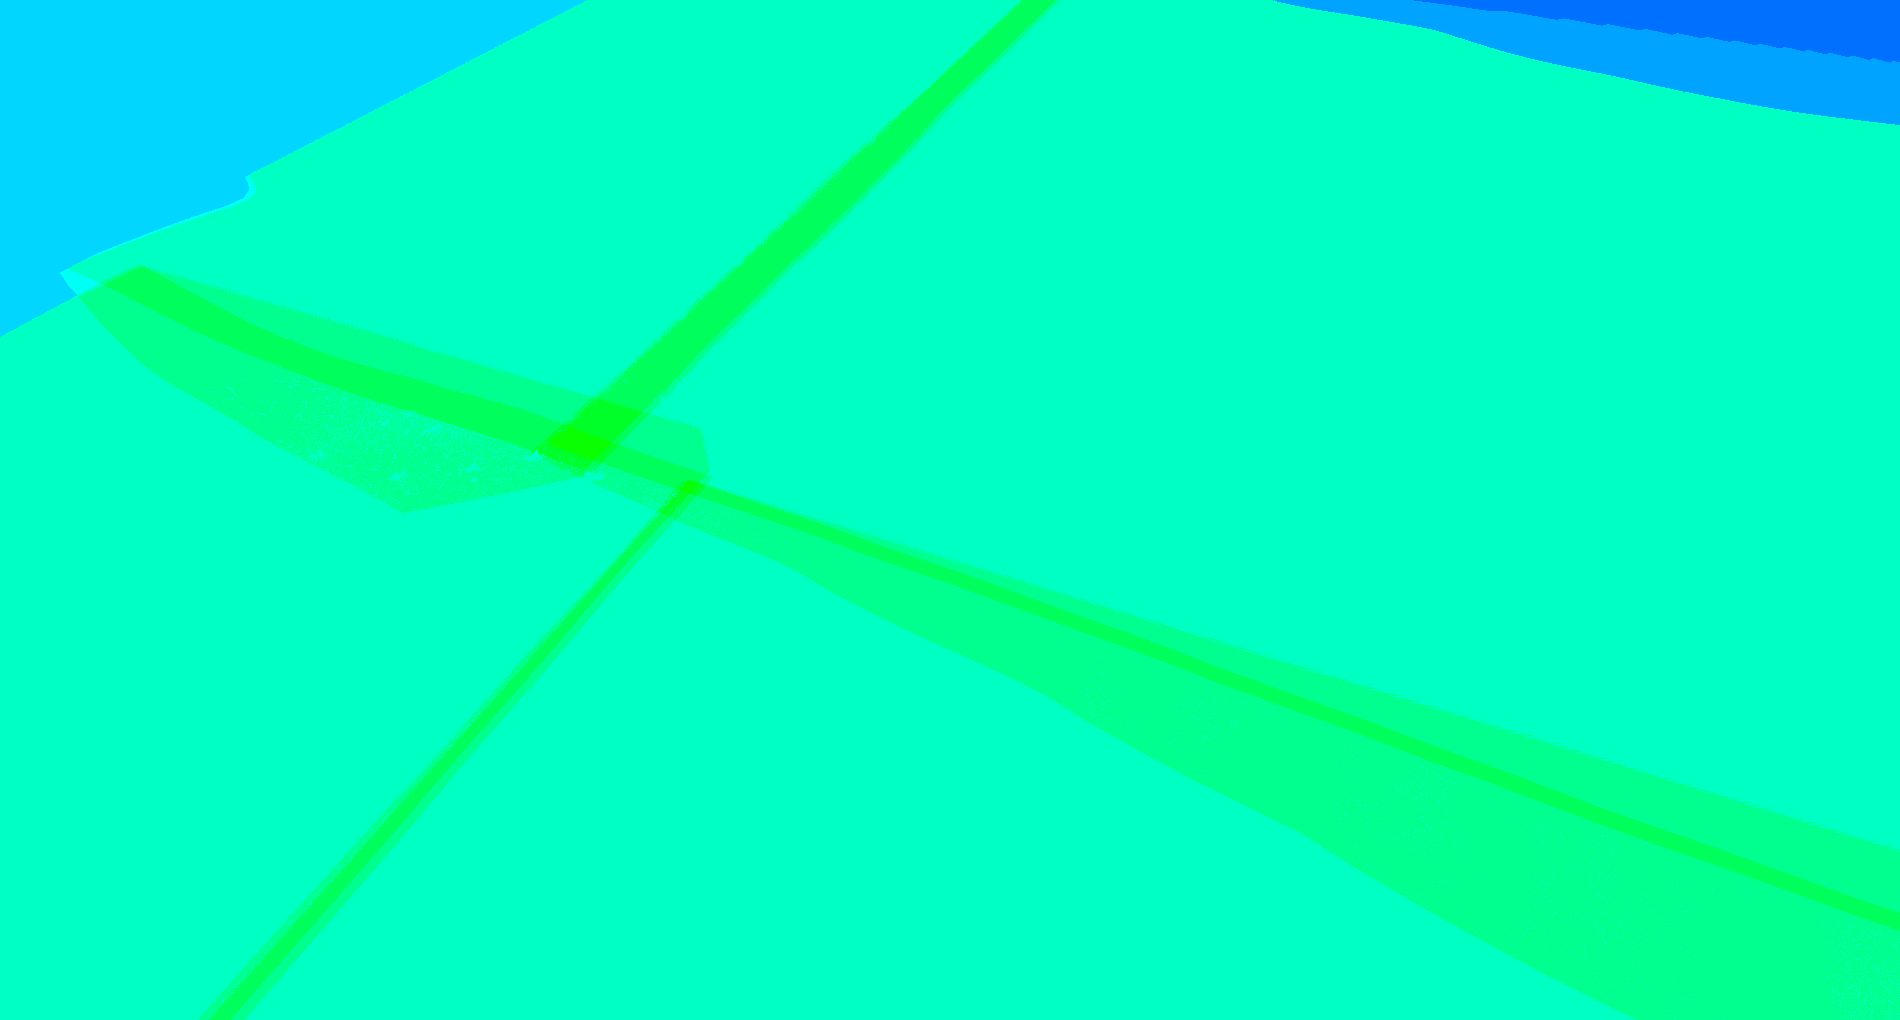
\includegraphics[width=.45\textwidth]{images/showcase/BeachMergedQuery128FPS.PNG}}
    \hfill
    \caption{Merging and then splitting results in less ray queries. Running @128FPS.}
    \label{fig:beachMerged}
\end{figure}
We are given a scene graph with a base geometry and an instance list for each instanced geometry. The issue now is that they too tend to overlap. As previously discussed, this leads to too many InstanceShader invocations than necessary. What then is possible is to merge all InstanceLists for a node into one which then requires only one InstanceShader invocation.\\
Note that there exists a limit on the number of instances that a scene can possess\ref{sec:BottleDeviceLimits}. Traversal shaders can bypass these limits by splitting the AABBs in such a way that they overlap as little as possible. The result can be something like \ref{fig:beachUnmerged} to \ref{fig:beachMerged}.
\newpage
\section{Using the Traversal Shader}
\label{sec:Usage}
Using the Traversal shader involves two steps. \\
First is modifying buffers and flagging nodes to indicate different behavior. PIs need to have even parity, else traversal shader is not invoked for these nodes. For this use a flag field in the scene node struct or define Boolean values.\\
The second step is modifying the InstanceShader function by implementing if-cases based on the nodes flags or bools.
\subsection{Multi-Level Instancing}
\label{sec:ImplMuliLevelInstancing}
The way traversal is executed in this shader easily allows for multi-level instancing. It supports the native instancing on even to odd levels. Wrapping Acceleration structures into AABBs also allows for more traversal depths, all that needs to be done is do enqueue another payload with the TLAS that was referenced by the AABB/Even node. For a pseudo code implementation see \ref{sec:InstanceShader}. For the structure of instances Figure \ref{fig:TraversalHierarchy} should also give a good idea.
\subsection{Level of Detail}
\label{sec:ImplLevelOfDetail}
\begin{figure}[h]
    \centering
    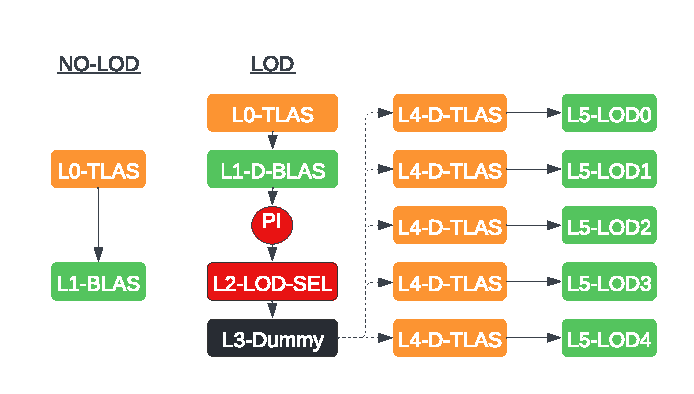
\includegraphics[width=.8\textwidth]{images/showcase/LOD-Select.pdf}
    \caption{Transformed scene graph for dynamic level of detail.}
    \label{fig:LODGraph}
\end{figure}
The current layout allows for a basic traversal through the scene graph with multi-level instancing. To now add more functionality into the traversal, it is necessary to flag nodes as specific types to indicate changed behavior. The example we will use is flagging nodes to select a Level-of-Detail for their children. First the scene node struct is added a new boolean field to indicates that a node is a LOD-Selector. These are predefined nodes that the scene compiler creates after we specify that we want a node to be a PI that selects a LOD. It is inserted in between the odd-geometry node and the even parent. Which means that in fact there must be two inserted nodes, since the parity constraint must hold, it is also necessary to consider the actual level that the node must have, which must be even. Because as stated previously: Traversal shader code can only be executed in the transition from odd to even level. 
\newpage
This leads to the insertion routine of a LOD-Selector S for a geometry node g (odd) as follows:
\begin{enumerate}
    \item Create an even LOD selector S node, that references g as LOD0
    \item For all parents of g replace g with with S as their child.
    \item Create levels of detail and add them to S as children in their order. With g as LOD0 being the highest LOD
    \item Let the constraint enforcer insert the dummies into the scene graph.
\end{enumerate}
Let's recap. An even node references odd geometry. A LOD-Selector does not execute traversal but instead selects another even node that has its own TLAS. This means that an odd dummy is inserted between each parent of g and the selector. Furthermore there is an odd dummy between the levels of Level-of-Detail and the selector. Lastly a Level-of-Detail consists of a TLAS that starts traversal and a BLAS as its only child that contains all geometry so that is another even and odd node added. This results in a graph like in \ref{fig:LODGraph}. Note that L2-LOD-SEL and L3-Dummy are nodes, but no AS is constructed for them. They exist for behavior and enforcing constraints.
\subsection{Other traversal functionality}
\label{sec:ImplOther}
Inserting more functionality follows the same principle. As the only things needing to be done is flag a node with a boolean or an integer flag, the last being better in the long run. Compiling the scene with the compiler and lastly adding an if clause in the InstanceShader to change traversal behavior. For example, it would be possible to flag a node as a portal, which transforms the ray to another position in the scene. Which then would have the effect of a portal. It is only necessary to pay attention to the AABBs and the t-Value in this case.
\section{Adjustments}
In this section I will present a few adjustments, which either prevent some artifacts or slightly improve performance further.
\subsection{Normal Transform}
\label{sec:NormalTransform}
Using a surface normal is essential for appropriate rendering. However, when rendering with this process there is no simple way to reconstruct the path which traversal took to reach to an instance. This was the reason that we used a worldToObject transform in the traversal shader instead of saving transformed origin and direction for the ray. That way at the end of the traversal the function also returns the final payload which then can be used to retrieve the node, intersection coordinates in world and object space as well as transforming the normal accordingly and the used LOD.
\subsection{Self occlusion}
\label{sec:SelfOcclusion}[h]
\begin{figure}
    \hfill
    \subfigure[Self occlusion]{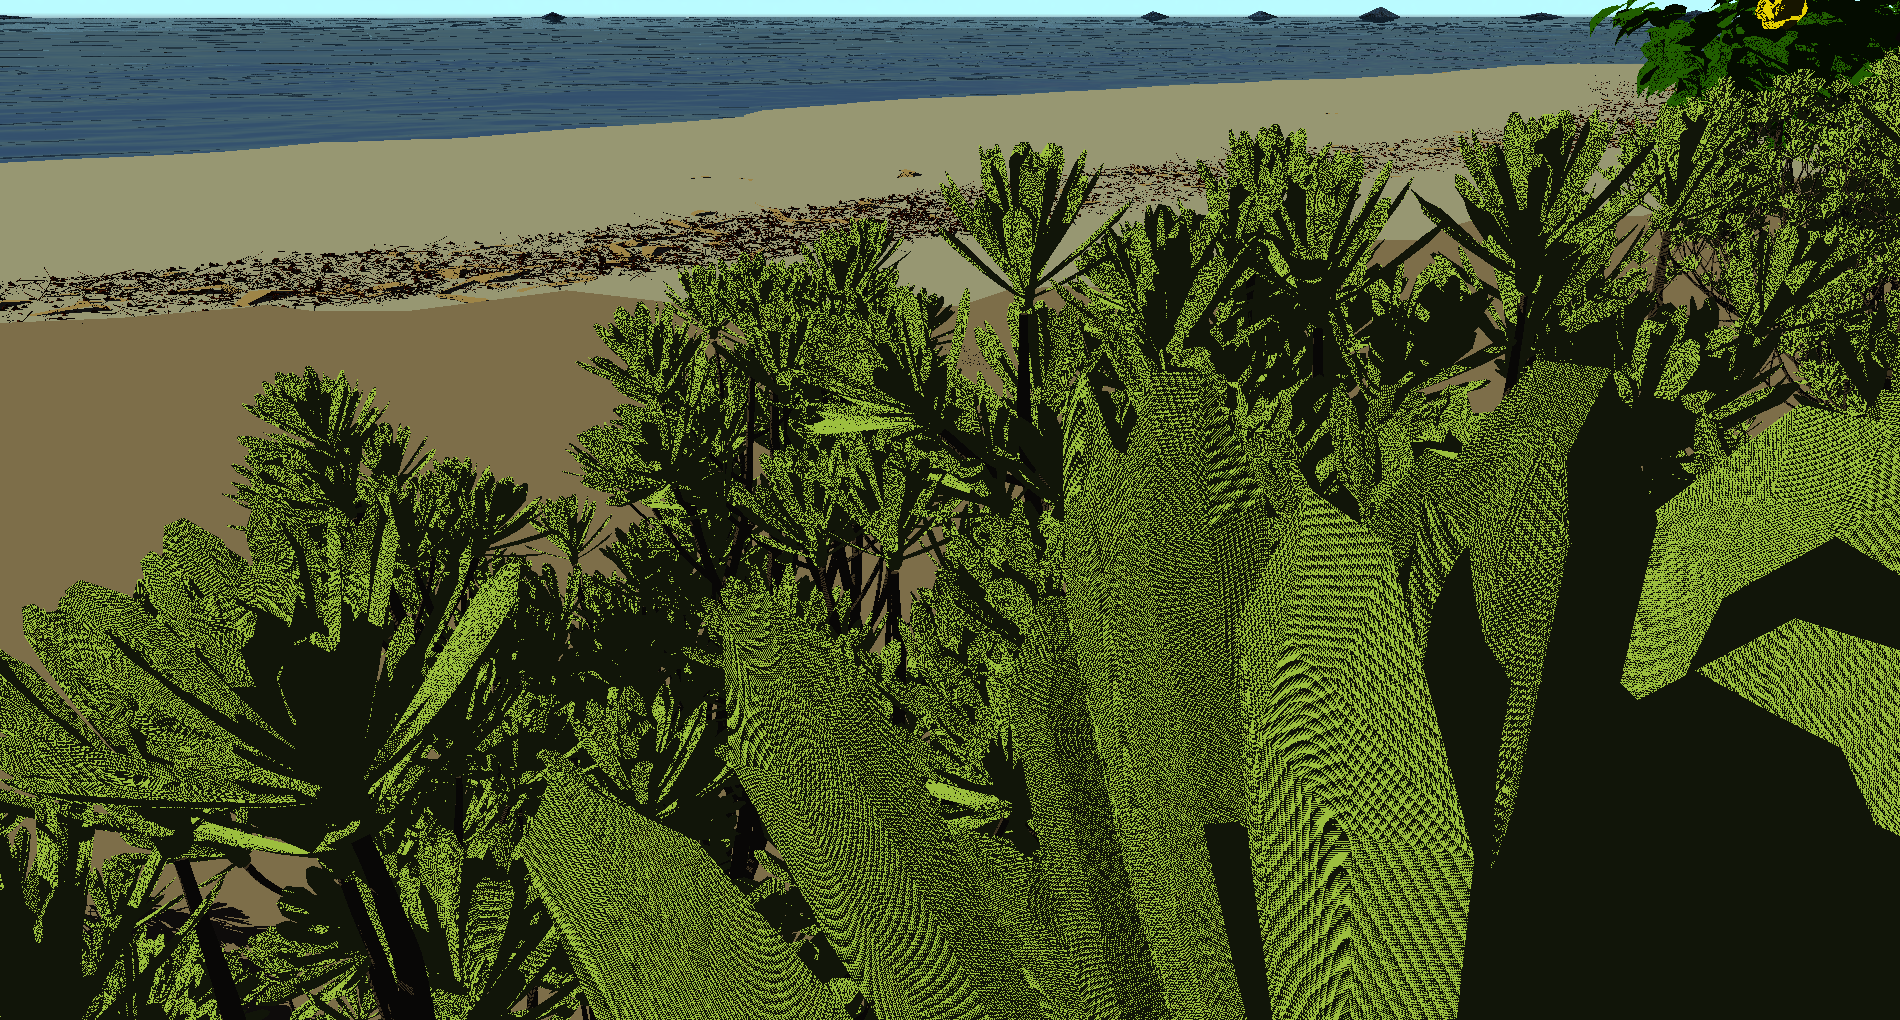
\includegraphics[width=.45\textwidth]{images/showcase/SelfOcclusion.PNG}}
    \hfill
    \subfigure[Fixed shadows]{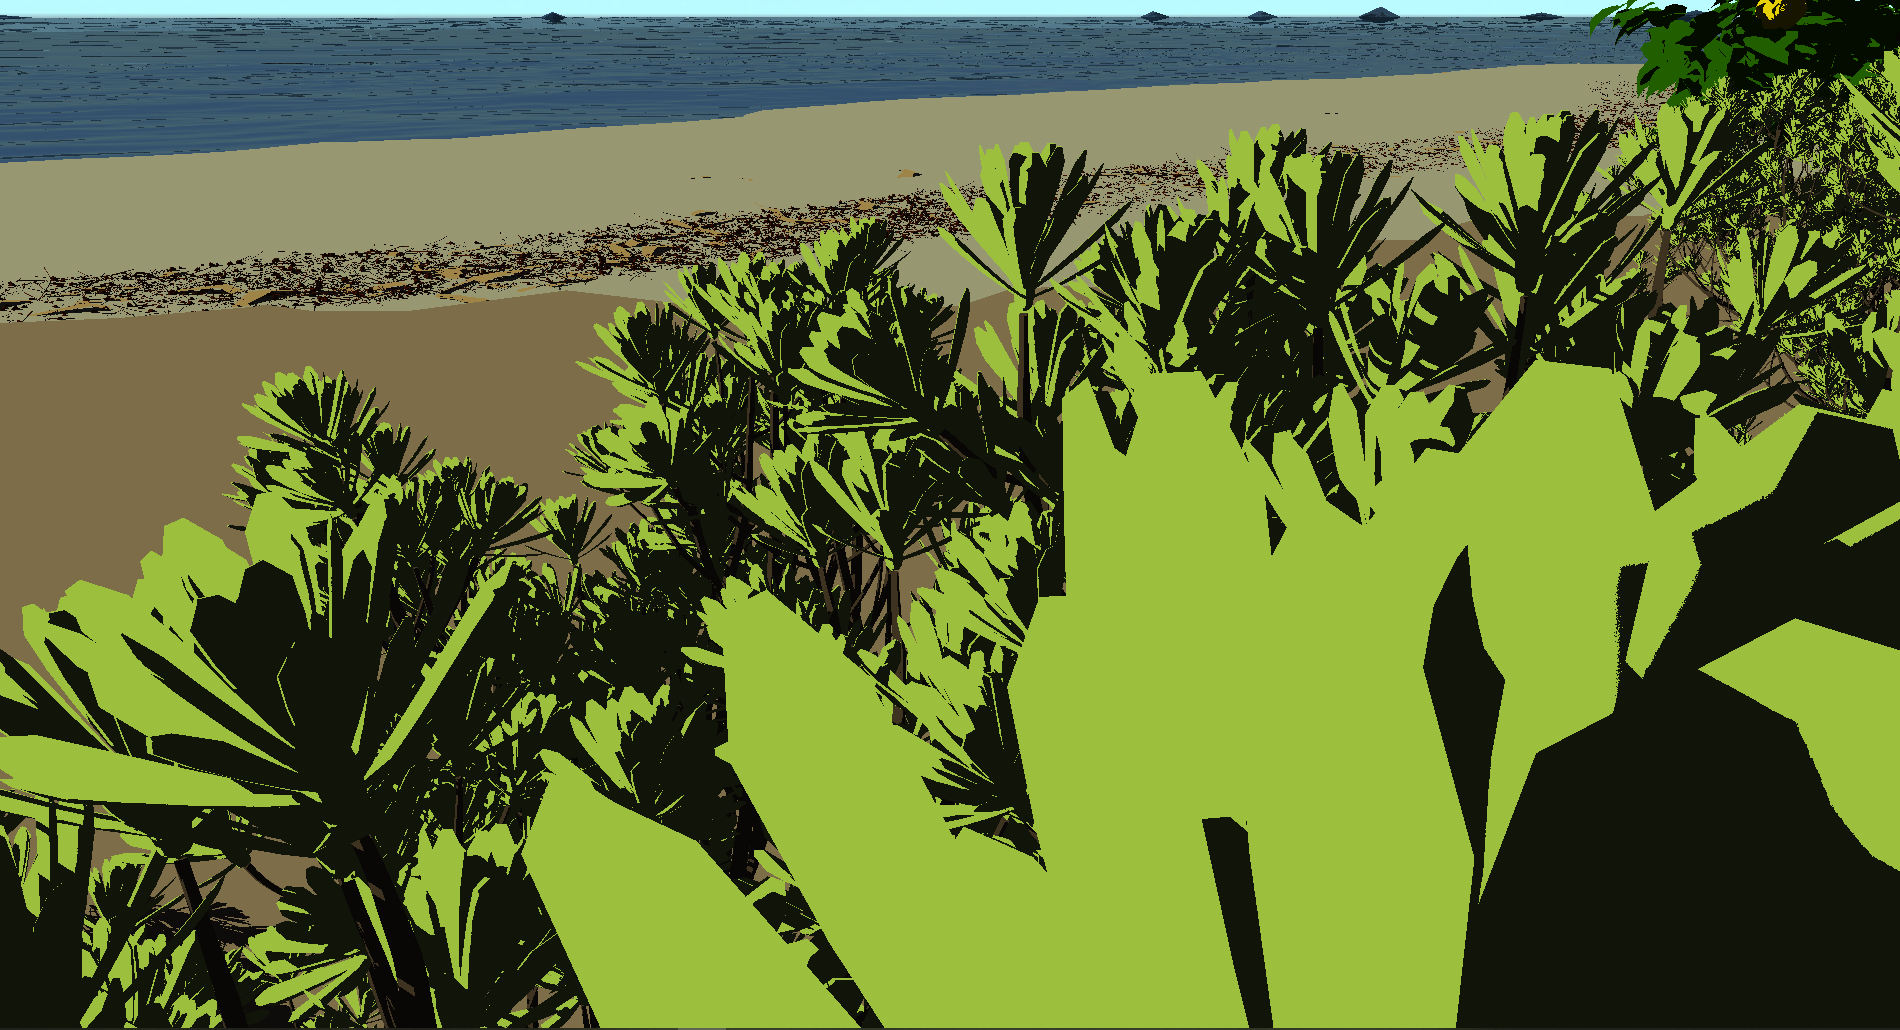
\includegraphics[width=.45\textwidth]{images/showcase/SelfOcclusionFixed.PNG}}
    \hfill
    \caption{Self occlusion caused by not offsetting intersection point.}
    \label{fig:SelfOcclusion}
\end{figure}
Self-occlusion is a common issue when raytracing. Most of the time be solved by offsetting tMin by a small margin. However, this is not feasible when there are significant size differences for triangles inside a scene, which is the case with our test set. Instead, the surface normal is used to offset the intersection by a small margin away from the surface, which is one of the reasons why the normal must be transformed into world space. The effects of this can be seen in \ref{fig:SelfOcclusion}.
\subsection{Level of Detail Artifacts}
\label{sec:LODArtifacts}
Level-of-Detail often suffers from a specific glitch, called the popping effect. This occurs when suddenly switching from one LOD to another. To prevent this from happening or minimize the visual effects, a common practice is using stochastic level of detail which stochasticly switches form one level of detail to another. This can be implemented with traversal shaders.\\
Additionally, LOD often has issues with self-occlusion (Fig \ref{fig:LODOcclusion}). This occurs if a primary ray intersects an object and the shadow ray uses another LOD than the primary ray. This can be solved by passing down the LOD into the traversal loop. With -1 indicating the use of a selected LOD and another value with the forced LOD level. The values are then passed on through the payloads and the finally used LOD is then returned by the result payload. Hence the comment for the TraversalPayload struct in \ref{sec:OptStackMemorySize}.
\begin{figure}[h]
    \hfill
    \subfigure[LOD-Self occlusion]{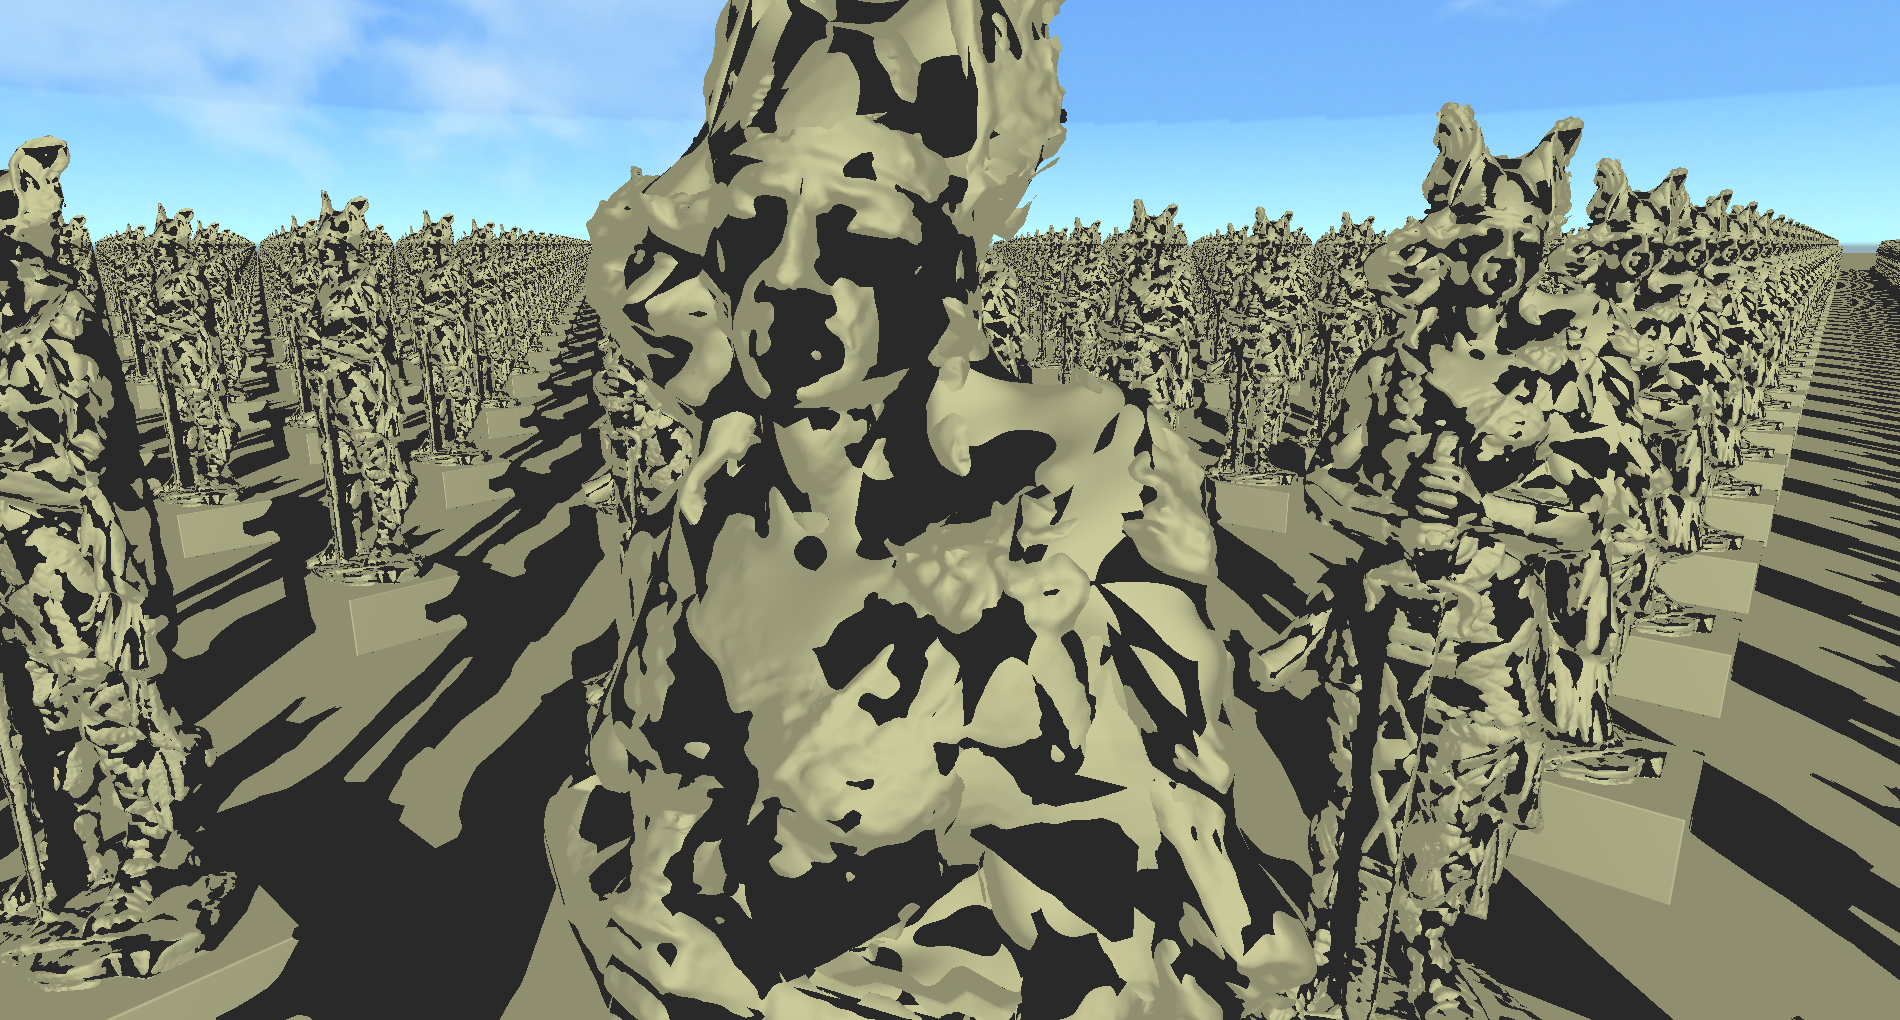
\includegraphics[width=.45\textwidth]{images/showcase/LOD-Occlude.PNG}}
    \hfill
    \subfigure[Fixed by forcing LOD for shadow rays]{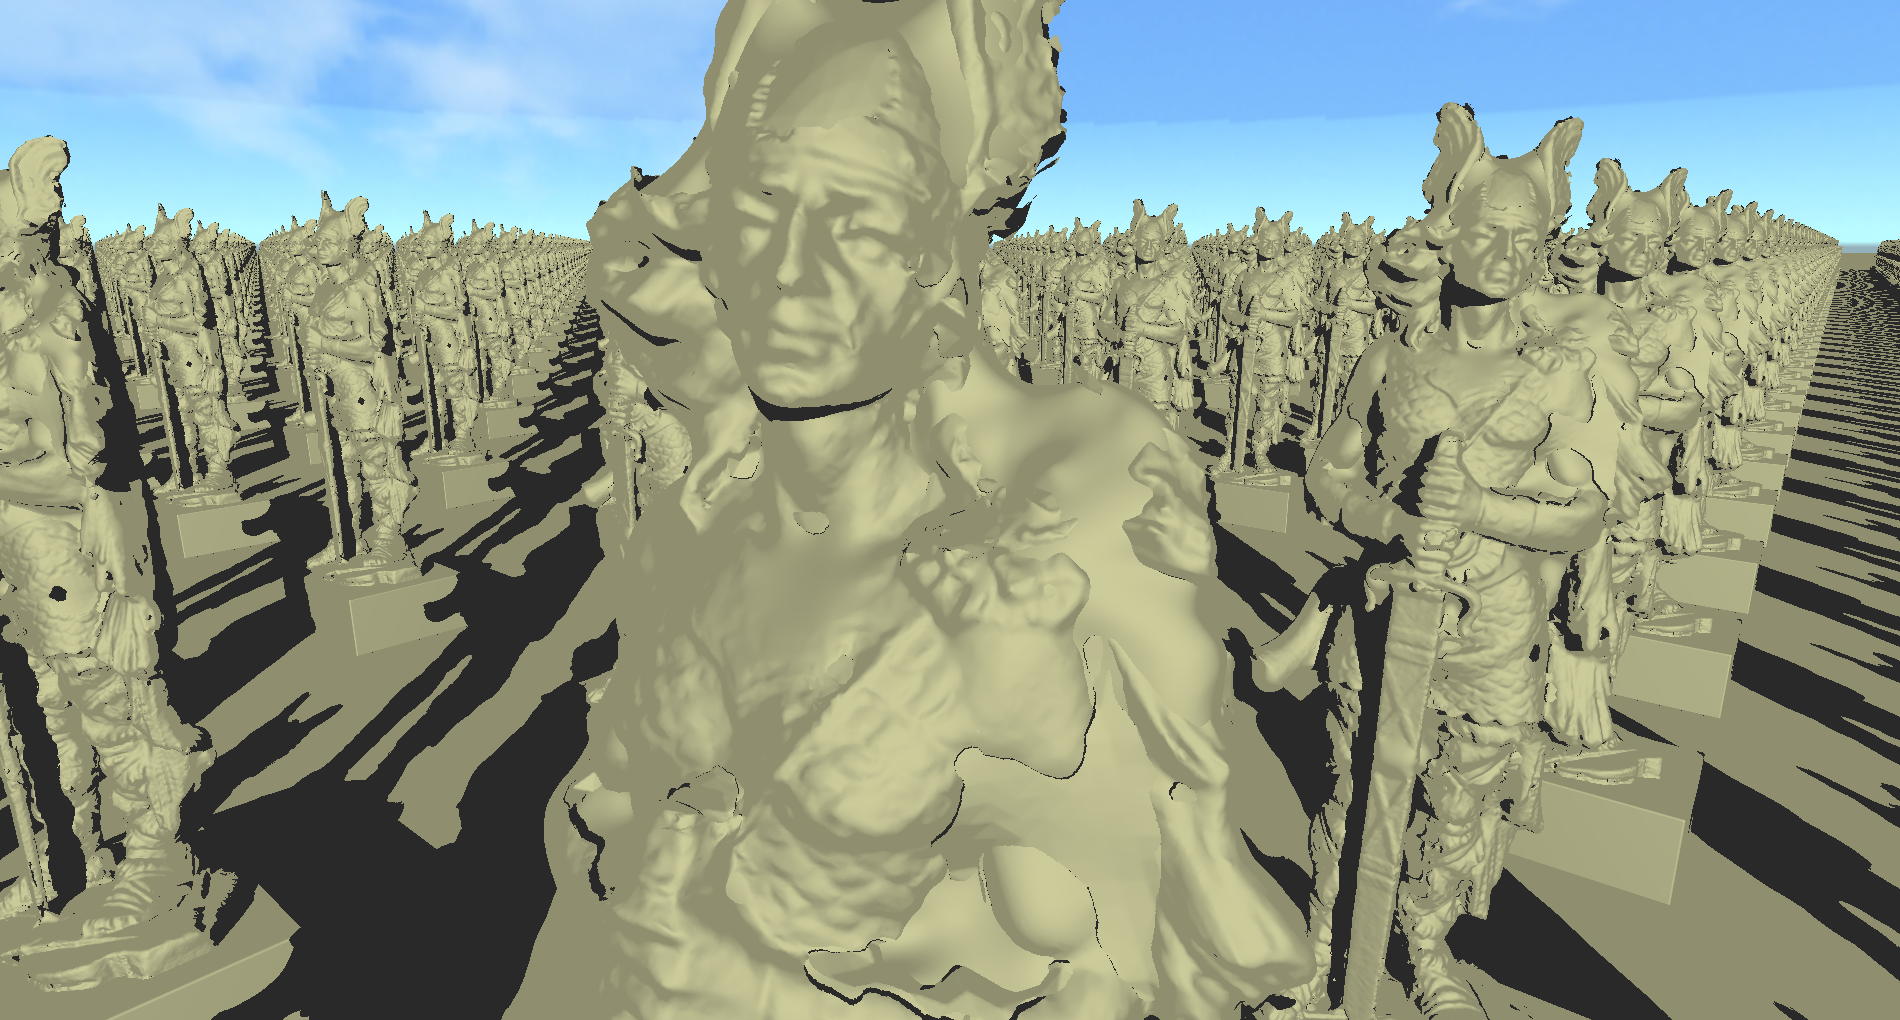
\includegraphics[width=.45\textwidth]{images/showcase/LOD-OccludeFixed.PNG}}
    \hfill
    \caption{Self occlusion caused by using the wrong LOD for shadow rays.}
    \label{fig:LODOcclusion}
\end{figure}
\subsection{Sm-Occupancy}
\label{sec:SmOccupancy}
One of the biggest problems when optimizing GPU computations is distributing work equally in such a way that all resources are used if possible. In testing the maximum warp occupancy that was reached was about 20\%. This is most likely due to only one RT-Core being available per SM thus limiting the amount of ray queries that can be run in parallel. This can be seen in \ref{fig:SMProfile} as the Pixel warps, which are the ones we run, only make less than 25\% of activity.
\newpage
\section{Final Layout}
\label{sec:FinalLayout}
In this section I will present the final layout of the traversal shader in GLSL code. First I will put the GLSL code and then go into detail. I will also reference the relevant chapters and sections for cross reference.
\subsection{Descriptors}
To understand the GLSL code I will use the actual buffer names as well as the function names. I will quickly list all descriptors and their names. For their usages see \ref{sec:SceneLayout}
\begin{itemize}
    \item buffer VertexBuffer vertices = $\mathbf{V}$
    \item buffer IndexBuffer indices = $\mathbf{T}$
    \item buffer NodeBuffer nodes = $\mathbf{N}$
    \item buffer TransfromBuffer transforms = $\{m | \exists  n \in \mathbf{N} : m = M(n)\}$
    \item buffer ChildBuffer childIndices = $\mathbf{C}$
    \item uniform accelerationStructureEXT[ ] tlas
\end{itemize}

\subsection{Traversal loop}
\label{sec:FinalTraversalLoop}
This is the loop that executes traversal and calls the InstanceShader() for intersected PIs. I will present all connected functions
\paragraph{Traversal Stack}
Let us first start with the traversal stack initialisation.
\begin{lstlisting}
struct TraversalPayload {// for the chosen layout see (*\ref{sec:OptStackMemorySize}*)
	mat4x3 world_to_object;
	float tNear; // the t for which this aabb was intersected
	int cIdx_nIdx; // after compute: node index; before compute: custom index
	int pIdx_lod; // after compute: LOD       ; before compute: primitve index
	int sIdx_un; // after compute: unsused   ; bebore compute: shaderOffset (grandchild)
};

const int TRAVERSAL_STACK_SIZE = 15;
int stackSize = 0; // on the usage of a stack see (*\ref{sec:Considerations}*)
TraversalPayload traversalStack[TRAVERSAL_STACK_SIZE];
\end{lstlisting}
This implements a stack with a maximum size, by updating the stackSize with every element added. The worldToObject matrix is necessary to transform the ray and later the normal.\\
t represents the AABBs t-Near value for skipping payloads, it is computed in the InstanceShader().
cIdx\_nIdx and pIdx\_lod are required to retrieve the intersected nodes and lastly sIdx is used as a value to denote another custom index, because instance lists use a transform node as well as the instanced node for which the BLAS will be traversed.
\newpage
\paragraph{Function Signature}
To now talk about the implementation of the traversal loop, lets first have a look at its signature
\begin{lstlisting}
bool ray_trace_loop(vec3 rayOrigin, vec3 rayDirection, 
float t_max, uint root, float minAlpha, int lod,
out vec3 tuv, out int triangle_index, 
out TraversalPayload resultPayload) {
\end{lstlisting}
The ray origin and direction are given in world space. tMax is the maximum distance a triangle hit is allowed. root is the index of the node from which traversal should start, in the most common case this is the root scene node. minAlpha denotes an alpha threshold for the triangle color for intersections to be committed. This can be used to simulate lighting though windows. lod is the forced LOD or -1 if none is forced. tuv represents a Vec3 that contains the result t-Value as well as the uv-coordinates for the triangle. triangleIndex is a pointer to the indexBuffer that allows to retrieve the triangle vertices and lastly the resultPayload is the payload of the closest traversal. It contains the node index and worldToObject transform.\\

\paragraph{Traversal initialisation}
Before traversal starts the stack must be initialized with the root node.
\begin{lstlisting}
tuv = vec3(0);
float min_t = 1.0e-4f;
float best_t = t_max; // our best_t which to keep decreasing
triangle_index = -1;// the index of the closest triangle, -1 to indicate no hit

TraversalPayload start; // start at root node
start.world_to_object = mat4x3(1);
start.cIdx_nIdx = int(root);
start.pIdx_lod = lod;
start.tNear = 0;
traversalStack[0] = start;

stackSize = 1;	
\end{lstlisting}
\newpage
\paragraph{Traversal loop}
\label{sec:ImplTraversalLoop}
This is the actual traversal loop that runs until the stack is empty. I will split this into two parts to make it easier to overview. First comes the query initialization  and the loop and lastly the closest hit routine.
\begin{lstlisting}
while (stackSize > 0) {
	stackSize--; // remove last element
	TraversalPayload load = traversalStack[stackSize];
	
	// there was already a closer hit, we can skip this payload (*\ref{sec:OptTraversalSpeed}*)
	if (load.tNear >= best_t) continue;
	
	int start = stackSize;
	SceneNode node = nodes[load.nIdx]; // retrieve scene Node
	uint tlasNumber = node.TlasNumber; // TLAS(n)
	
	vec3 query_origin = (load.world_to_object * vec4(rayOrigin,1)).xyz;
	vec3 query_direction = (load.world_to_object * vec4(rayDirection,0)).xyz;
	
	// for the ray query initialisation see (*\ref{sec:TraversalLoop}*)
	rayQueryEXT ray_query;
	rayQueryInitializeEXT(ray_query, tlas[tlasNumber], 0, 0xFF,
		query_origin, min_t,
		query_direction, best_t);

	while (rayQueryProceedEXT(ray_query)) {
	    // runs the ray query. For an elaboration see (*\ref{sec:ImplQueryLoop}*)
	}
	// tells us how many instances were added
	int end = stackSize;
	int added = end - start;
	
	// runs the instance shader for all intersected PIs
	// it was moved out of the query loop for performance. See (*\ref{sec:OptQuerySpeed}*)
	for(int i = start;i < end;i++) {
		// See (*\ref{sec:ImplInstanceShader}*)
		InstanceShader(node, i, rayOrigin, rayDirection, load.pIdx_lod);
	}
	
	// inverts the added payloads such that the top payload in the 
	// stack has probably the lowest t-Value. See (*\ref{sec:OptTraversalSpeed}*)
	for (int i = 0; i < added / 2; i++) {
		int i1 = start + i;
		int i2 = end - 1 - i;
		TraversalPayload tmp1 = traversalStack[i1];
		TraversalPayload tmp2 = traversalStack[i2];
		traversalStack[i1] = tmp2;
		traversalStack[i2] = tmp1;
	}
	
	if (commitedType == gl_RayQueryCommittedIntersectionTriangleEXT) {
		// process closest intersection. See (*\ref{sec:ImplClosestHit}*)
	}
}
\end{lstlisting}

First the payload is retrieved, then it is checked against the current best\_t and skipped if possible. Otherwise, the node is retrieved and the ray is transformed into node-object space and the ray query is initialized and started. Once it finishes, first, all instance hits are computed and after that the added payloads are reversed to speed up convergence. The payloads are added, or more precisely their data to be processed is set inside the query loop which I will talk about next. Just note that the function call of InstanceShader processes the payload, for further info see \ref{sec:ImplInstanceShader}.
\newpage
\paragraph{Query loop}
\label{sec:ImplQueryLoop}
The query loop runs the ray query and processes the triangle intersections or adds the data for the InstanceShader for each intersected PI to the stack to be processed afterwards\ref{sec:OptQuerySpeed}.
\begin{lstlisting}
while (rayQueryProceedEXT(ray_query)) {
    // determine candidate intersection type.
	uint type = rayQueryGetIntersectionTypeEXT(ray_query, false);
	switch (type) {
	case gl_RayQueryCandidateIntersectionTriangleEXT:
#ifdef OPAQUE_CHECK	
		// checks if the triangle hit is opaque. 
		// Can impact performance significantly
		triangleHit(ray_query, node, minAlpha);
		break;
#else
		// always commit if opaque check is disabled
		rayQueryConfirmIntersectionEXT(ray_query);
		break;
#endif
	case gl_RayQueryCandidateIntersectionAABBEXT:
	    // if the stack exceeds its maximum size, the only option is to skip adding more payloads.
	    // for what happens in that case see (*\ref{sec:BottleStackSize}*)
		if(stackSize>=TRAVERSAL_STACK_SIZE)
			break;
		// the shader passes all relevant values into a new payload, 
		// which later uses these to run the instance shader, 
		// it adds the parent payload and the required RayQuery parameters
		// for why the instanceShader is not here see (*\ref{sec:OptQuerySpeed}*)
		// for their use inside the InstanceShader see (*\ref{sec:ImplInstanceShader}*)
		traversalStack[stackSize] = load;
		traversalStack[stackSize].cIdx_nIdx = rayQueryGetIntersectionInstanceCustomIndexEXT(ray_query, false);
		traversalStack[stackSize].pIdx_lod = rayQueryGetIntersectionPrimitiveIndexEXT(ray_query, false);
		traversalStack[stackSize].sIdx_un = int(rayQueryGetIntersectionInstanceShaderBindingTableRecordOffsetEXT(ray_query, false));
		stackSize++;
		break;
	default: break;
	}
}
\end{lstlisting}
The ray query loop runs until no further triangles are found, then it switches based on the type of intersection and either processes a triangle hit or adds a new payload for the intersected PI. The closest triangle hit is then processed after the ray query finishes, which I come to now.
\newpage
\paragraph{Closest hit update}
\label{sec:ImplClosestHit}
If a RayQuery intersected a triangle its intersection is processed after the query loop and the InstanceShader() calls \ref{sec:TraversalLoop}. After that comes the update of the closest hit.

\begin{lstlisting}
// check if there was a commited triangle intersection
float t = rayQueryGetIntersectionTEXT(ray_query, true);
if (t < best_t) {
	// updates the tuv return value and the best_t
    best_t = t;
	tuv.x = t;
	
	// retrieve the BLAS node in which the intersection occured
	SceneNode blasChild;
		
	// instance lists use the shaderBindingOffset to denote the 
	// BLAS and custom index for the transfrom
	if(node.IsInstanceList){
		blasChild = nodes[rayQueryGetIntersectionInstanceShaderBindingTableRecordOffsetEXT(ray_query, true)];
	}
	else {
	    blasChild = nodes[rayQueryGetIntersectionInstanceCustomIndexEXT(ray_query, true)];
	}
		
	// updates the triangle index and the uv coordiantes
	triangle_index = blasChild.IndexBufferIndex / 3 +
		rayQueryGetIntersectionPrimitiveIndexEXT(ray_query, true);
	vec2 uv = rayQueryGetIntersectionBarycentricsEXT(ray_query, true);
	tuv.y = uv.y;
	tuv.z = uv.x;
			
	// updates the result payload which is returned
	mat4 world_to_object = mat4(rayQueryGetIntersectionWorldToObjectEXT(ray_query, true));
	resultPayload.cIdx_nIdx = blasChild.Index;
	resultPayload.world_to_object = mat4x3(world_to_object * mat4(load.world_to_object));
	resultPayload.tNear = best_t;
	resultPayload.pIdx_lod = load.pIdx_lod;
}
\end{lstlisting}

First the triangle t-Value is compared and updated, after that the scene node is retrieved and using its data the return values are updated. Triangle hits normally occur only as the Level increases, therefore, the InstanceShader gets invoked at low levels.
\newpage
\paragraph{Return value}
The method returns and passes its output via the constantly updated out values, which are updated whenever a closer hit is found. Whether a triangle intersection occurred or not is determined by \texttt{return triangle\_index >= 0}. This finishes the implementation of the traversal loop. Up next is the actual InstanceShader which can be used to emulate a traversal shader.

\subsection{Instance shader}
\label{sec:ImplInstanceShader}
The instance shader is responsible to update the payloads from the unprocessed values to the actually computed payloads which are then used to continue traversal. Like in \ref{sec:FinalTraversalLoop} I will first start with the function signature.
\paragraph{Function Signature}
The function signature is as follows:
\begin{lstlisting}
void instanceShader(SceneNode tlas, int index, 
        vec3 rayOrigin, vec3 rayDirection, 
        int parentLOD){	
	TraversalPayload nextLoad = traversalStack[index];
    ...
}
    
\end{lstlisting}
tlas is the TLAS scene node in which the BLAS for the PI is contained. index is the index into the stack to indicate which Payload to process and rayOrigin and rayDirection are the ray parameters in world space to be used to compute the t-Value for the payload. Using the index, the function then retrieves the payload to process from the stack (without removing it). ParentLOD is the passed down LOD for the payload which is used for the selection of the LOD \ref{sec:ImplLevelOfDetail}.
\newpage
\paragraph{BLAS and PI retrieval}
First thing to do is retrieve the BLAS node and the PI node, only then can different traversal behavior be modeled. The function uses the saved index data of the ray query to retrieve these values. InstanceLists hereby play a role as they behave differently, since the first child is only the transform and the second is the BLAS. The same goes for PIs in BLASs which are marked as an InstanceList. It is also necessary to keep track of the transforms, and in which order they are applied.

\begin{lstlisting}
// the direct child is referenced by the custom index 
// this is defined during the TLAS build. See (*\ref{sec:TraversalTreeBuild}*)
SceneNode blas;
// checks if the TLAS is an instance List
if(tlas.IsInstanceList)	{
    // the instance is the instance with the transformation
	SceneNode instance = nodes[nextLoad.cIdx_nIdx];
	blas = nodes[nextLoad.sIdx_un];
	// update the world_to_object matrix to transform into BLAS object space
	world_to_object = mat4x3(
	    mat4(inverse(transforms[blas.TransformIndex])) *
	    mat4(inv(transforms[instance.TransformIndex]))
	);
} else {
	blas = nodes[nextLoad.cIdx_nIdx];
	// update the world_to_object matrix to transform into BLAS object space
	world_to_object = inv(transforms[blas.TransformIndex]);
}

// get the PI
SceneNode next;
// checks if the BLAS is an instance list
if(blas.IsInstanceList){
    // a dummy exists for the instances because:
    // BLAS->odd, PI->even, instance is in between, therefore dummy is
    // inserted between BLAS and instances, dummy references the instances then
    // results in: BLAS->Dummy->Instances->PIs
    // a dummy also exists for TLAS instance lists, however it is skipped by 
    // using the custom index
	SceneNode dummy = nodes[childIndices[blas.ChildrenIndex]];
	SceneNode instance = nodes[childIndices[dummy.ChildrenIndex+nextLoad.pIdx_lod]];
	next = nodes[childIndices[instance.ChildrenIndex]];
	// update the world_to_object matrix to transform into PI-object
	world_to_object = mat4x3(
	    mat4(inv(transforms[instance.TransformIndex])) * 
	    mat4(world_to_object)
	);
} else {
	// update the world_to_object matrix to transform into PI-object
	next = nodes[childIndices[blas.ChildrenIndex + nextLoad.pIdx_lod]];
}
\end{lstlisting}

The first part is retrieving the BLAS-Node. This is by using the custom index and if the TLAS is an instance list, using the shaderIndex to specify which child of the instance is actually meant. For the usage of instance lists see \ref{sec:OptStackSize}. Something like the sIdx is not available for the BLAS, therefore, for the child not to be ambiguous there must only be one child per instance. Other than that, the world\_to\_object transform gets updated to transform the ray into object space.
\newpage
\paragraph{AABB intersection}
Next up is computing the t-Value for the payload. This requires the ray in object coordinates. For that the world ray has been passed and the parent payload with the world\_to\_object matrix can be used. The AABB is then intersected and the tNear value is set as the t-Value for the payload since it is the minimum distance at which a triangle hit can occur in this PI.

\begin{lstlisting}
// transforms the ray into object space
vec3 origin = world_to_object * vec4(nextLoad.world_to_object * vec4(rayOrigin,1),1);
vec3 direction = world_to_object * vec4(nextLoad.world_to_object * vec4(rayDirection,0),0);

// computes the AABB intersection using the AABB of the PI 
// as well as the transformed origin and direction.
float tNear, tFar;
intersectAABB(origin, direction, next.AABB_min, next.AABB_max, tNear, tFar);
\end{lstlisting}

The AABB intersection algorithm is as follows \cite{pbrBook}.
\begin{lstlisting}
bool intersectAABB(vec3 rayOrigin, vec3 rayDir, vec3 boxMin, vec3 boxMax, 
        out float tNear, out float tFar) {
	vec3 tMin = (boxMin - rayOrigin) / rayDir;
	vec3 tMax = (boxMax - rayOrigin) / rayDir;
	vec3 t1 = min(tMin, tMax);
	vec3 t2 = max(tMin, tMax);
	tNear = max(max(t1.x, t1.y), t1.z);
	tFar = min(min(t2.x, t2.y), t2.z);
	// AABB is intersected if tNear is <= tFar
	return tNear<=tFar;
}
\end{lstlisting}
\newpage
\paragraph{LOD-Selector implementation}
\label{sec:ImplLOD}
The instance shader that is implemented has LOD selection support. For this a boolean field in the scene node is retrieved and if the PI is a LOD selector it sets the TLAS to traverse next. The selection function for the LOD uses a projection of the object onto the screen. This is the inserted statement after the determination of the PI in the InstanceShader() function.
\begin{lstlisting}
// sets the used LOD to the parent LOD
int lod = parentLOD;
// checks if the PI is an instance selector
if(next.IsLodSelector) {
    // selects a LOD to traverse next
	mat3 tr = mat3(world_to_object * mat4(nextLoad.world_to_object));
	next = selectLOD(next,tNear, tr, parentLOD, lod);
}
\end{lstlisting}
And the called function:
\begin{lstlisting}
SceneNode selectLOD(SceneNode selector, float tNear, mat3 tr, 
        int parentLOD, out int lod){
	SceneNode dummy = nodes[childIndices[selector.ChildrenIndex]];
	int N = dummy.NumChildren;
	if(parentLOD >= 0) {
		lod = parentLOD;
	} else {
	    // calculates the radius of an encapsulating sphere
		float rObject = length(selector.AABB_max-selector.AABB_min)/2;
		float rMax = 5000;
		float t = max(0,tNear);
		// projects the sphere onto screen space
		float rPixel = rObject * height / (tan(PI / 180 * fov) * 2 * t);
		// selects LOD bases on rPixel
		lod = -int(log2(pow(2,N-1) * rPixel/rMax));
		lod = max(lod, 0);
	}
	lod = min(lod, N-1);
	return nodes[childIndices[dummy.ChildrenIndex + lod]];
}
\end{lstlisting}

After this the node next is the TLAS for the geometry, which can then be traversed once the traversal loop runs for that payload.
\newpage
\paragraph{Payload update}
Lastly the payload must be updated for traversal to function properly.
\begin{lstlisting}
// computes the world to object from TLAS space 
// to the space of the node next(without its transform)
world_to_object = mat4x3(mat4(inv(transforms[next.TransformIndex])) 
                       * mat4(world_to_object));

// sets the node index
nextLoad.cIdx_nIdx = next.Index;
// computes the transform from the world space to the node
nextLoad.world_to_object = mat4x3(mat4(world_to_object) 
                                * mat4(nextLoad.world_to_object));
// the hit can be discarded by setting t to a high value
nextLoad.t = tNear;
// saves the used LOD to be used for lower nodes
nextLoad.pIdx_lod = lod;
// updating the entry
traversalStack[index] = nextLoad;
\end{lstlisting}

Every acceleration structure is in the space of the defining node without the node transform. since the transform denotes the position relative to any parent. However, traversing the structure should be independent from any parent therefore it is in object space of the node.

\subsection{Recap}
This makes the implementation of the Traversal shader in GLSL. Let's recap the required functions quickly:
\begin{itemize}
    \item TraversalLoop - executes the traversal until the stack is empty. This is the entry point. \ref{sec:ImplTraversalLoop}
    \item InstanceShader - computes the nodes to traverse next after the query has finished with the saved values. \ref{sec:ImplInstanceShader}
    \item selectLOD - selects a level of detail for a given LOD-Selector, this is an implementation of LOD for a traversal shader. \ref{sec:ImplInstanceShader}
\end{itemize}
Next up is testing this implementation.

\chapter{Evaluation}
In this chapter we will take a look at the shader performance by using test data. We will be toggling on and off some of the optimizations we made in the previous chapter and take a look at their performance. For testing we use a Nvidia RTX 3060. The application runs almost solely on the GPU, say except for setting the uniform and applying camera movement. We will use a simple instantiation for a high-resolution mesh when testing for LOD. For multi-level and single-level instancing we will use the BayCedar of Moana Island. Lastly, we will test the shader on the Moana Island scene using a bunch of different configurations. All tests use 1920x1080 resolution. Note that for all tests here the opaque check is removed! This is due to it significantly slowing down ray queries in some cases. Instead, the triangle intersection is just commited. Transparency is simulated with secondary rays. Therefore, the rendered image stays the same. We will look at:
\begin{itemize}
    \item Frame rate - this is the most significant statistic as it determines usability for real time application. This is determined by the application frame rate display.
    \item GPU Memory - this is significant when using multi-level instancing as it is a technique to allow for lower memory usage. This gives us the ability to scale the scene exponentially. Memory hereby refers to the descriptor buffers and the buffers for the acceleration structures. This value is given by the application, it prints out the scene size on the GPU.
    \item Cache-Efficiency -tells us how performant the memory accesses are for the application, it is obtained by the GPU trace from Nvidia Nsight Graphics.
    \item Pixel-Warps - tells us how much of the GPU computation power we are actually using. This value is also obtained by the GPU trace from Nvidia Nsight Graphics.
    \item RQ-Stall - Nvidia Nsight Graphics gives the utility to profile shader performance and identify performance bottlenecks.The RQ-Stall hereby refers to the call of RayQueryProceedEXT() and how much shader time is spent executing this function.

\end{itemize}
\newpage
\section{Moana Island}
\begin{figure}
    \centering
    \subfigure[Overlook]{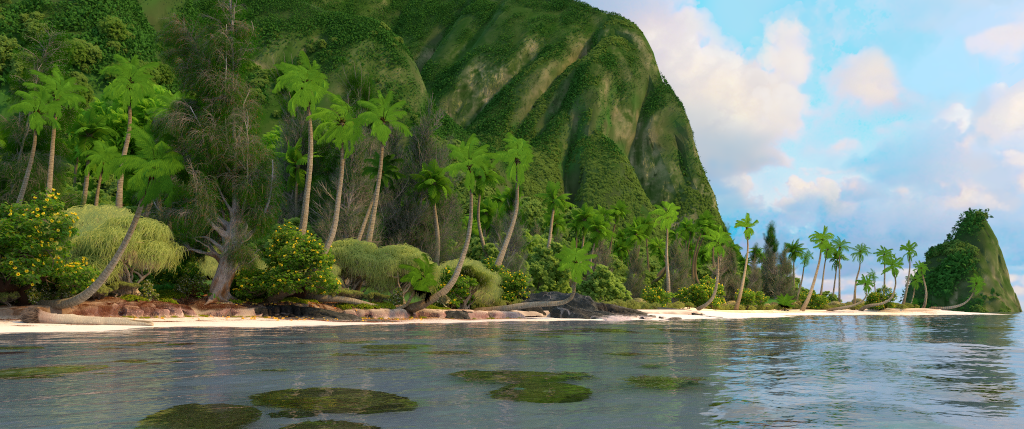
\includegraphics[width=.7\textwidth]{images/showcase/Moana shotCam.png}}
    \subfigure[Beach view]{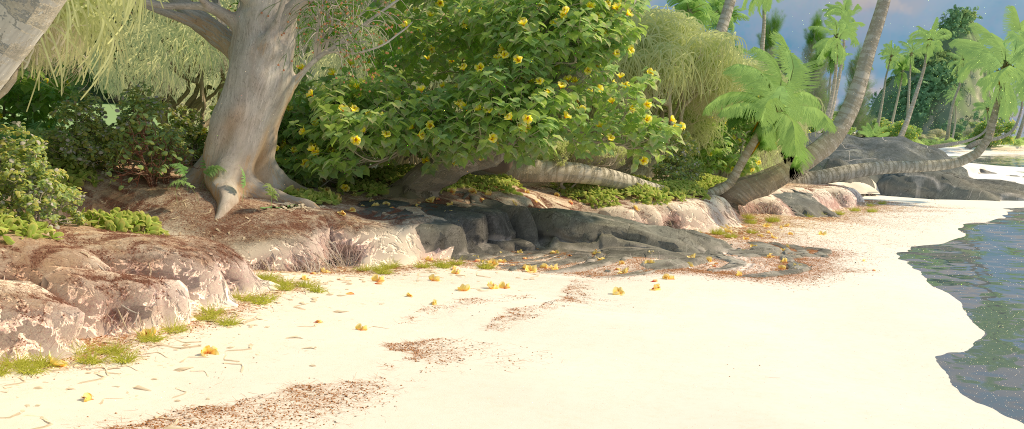
\includegraphics[width=.7\textwidth]{images/showcase/Moana beachCam.png}}
    \caption{Images of Moana island. Source:pbrt-images of Moana Island Dataset.}
    \label{fig:moanaPBRTRender}
\end{figure}
Moana island\cite{moanaIsland} is an open access Disney production asset. It features an island with high resolution meshes, multi-level instancing, the ptex texture format and much more. It consists of various sections that specify a specific part of the scene. UV-Textures are not used, as the ptex format is a per quad format which is difficult to implement and consumes quite a bit of memory. Figure \ref{fig:moanaPBRTRender} shows a full render of Moana Island, which is not quite feasible in our case. Instead, we will render most of the geometry but skip out on textures. The size of Moana Island exceeds 30M instances, 70M triangle primitives, 1.1B vertice and a total triangle count of over 30B. For our purposes this would require 5 TLAS and 313 BLAS. Unfortunately this scene is still too large to handle (10GB in byte buffer format) so we will only be able to render parts of it.
\newpage
\section{Level of Detail}
\label{sec:LODTEST}
First, we test Level-of-Detail to improve performance when using far away objects as described in \ref{sec:LOD}.
\subsection{Setup}
\begin{figure}
\hfill
\subfigure[Rendered image]{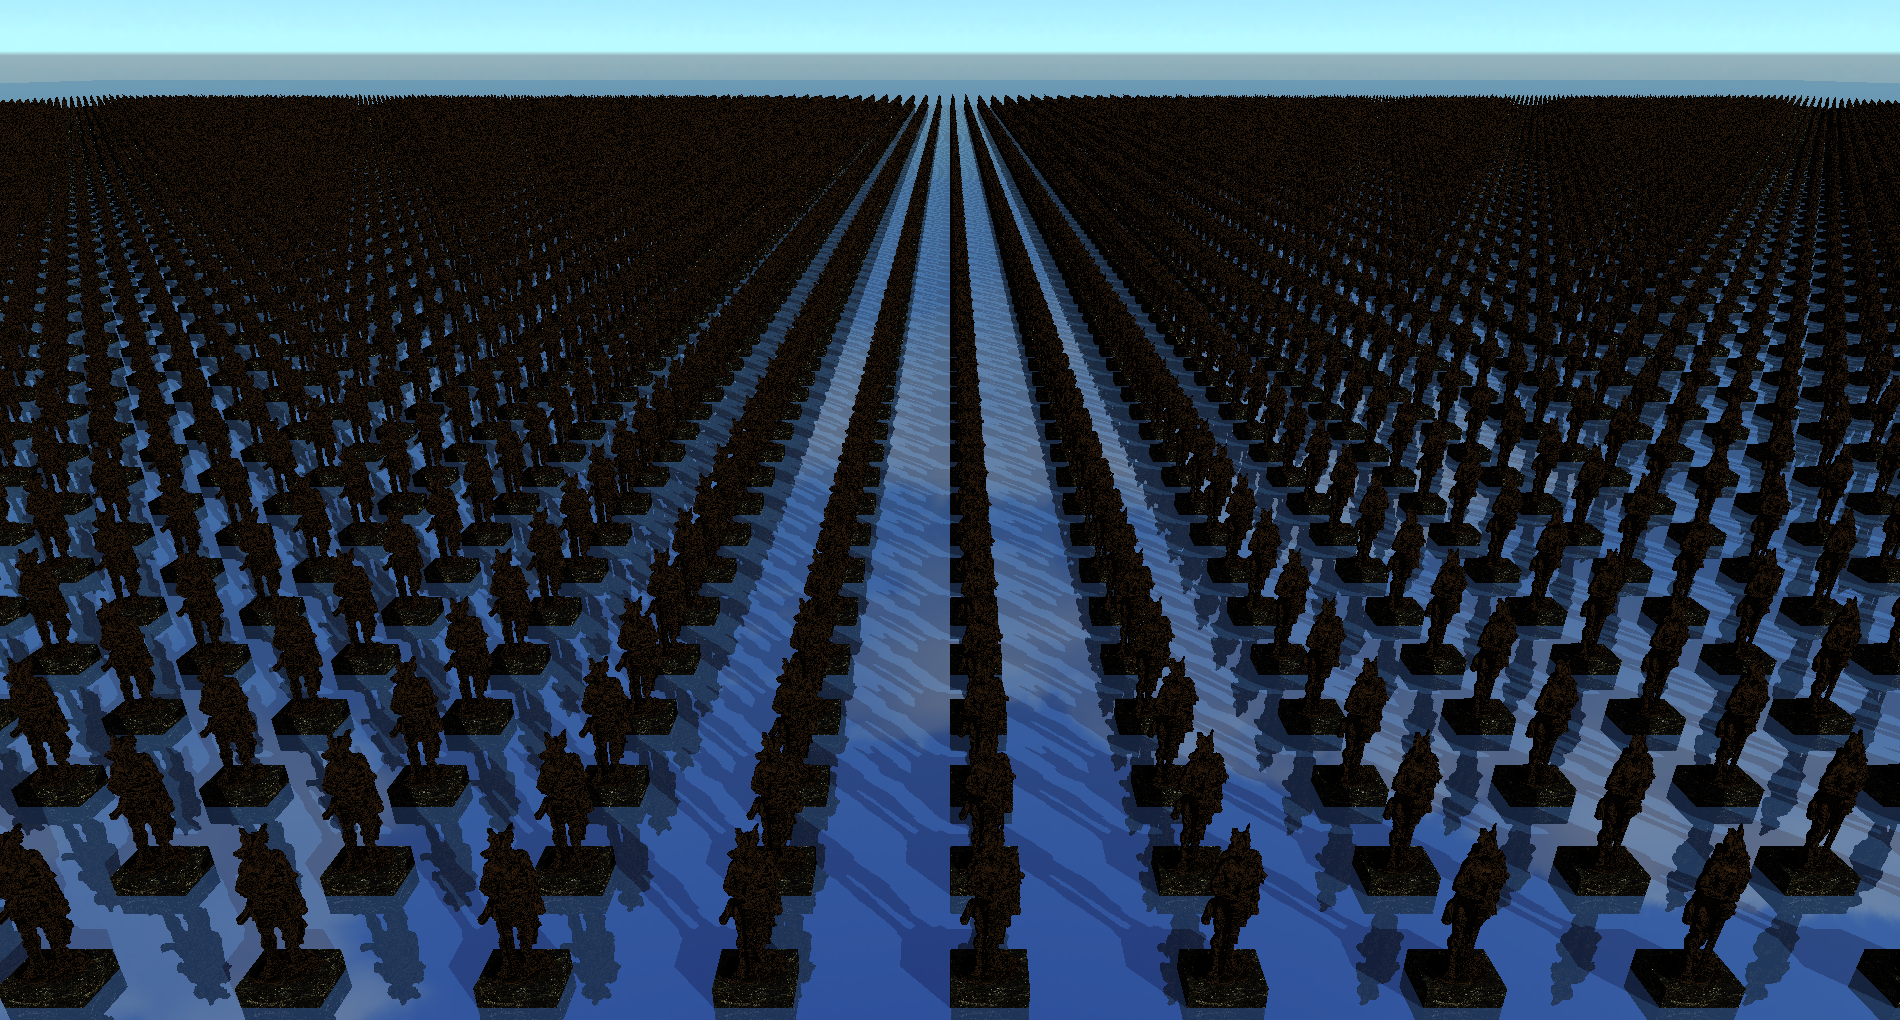
\includegraphics[width=.45\textwidth]{images/testing/LOD Render.PNG}}
\hfill
\subfigure[Displayed LOD]{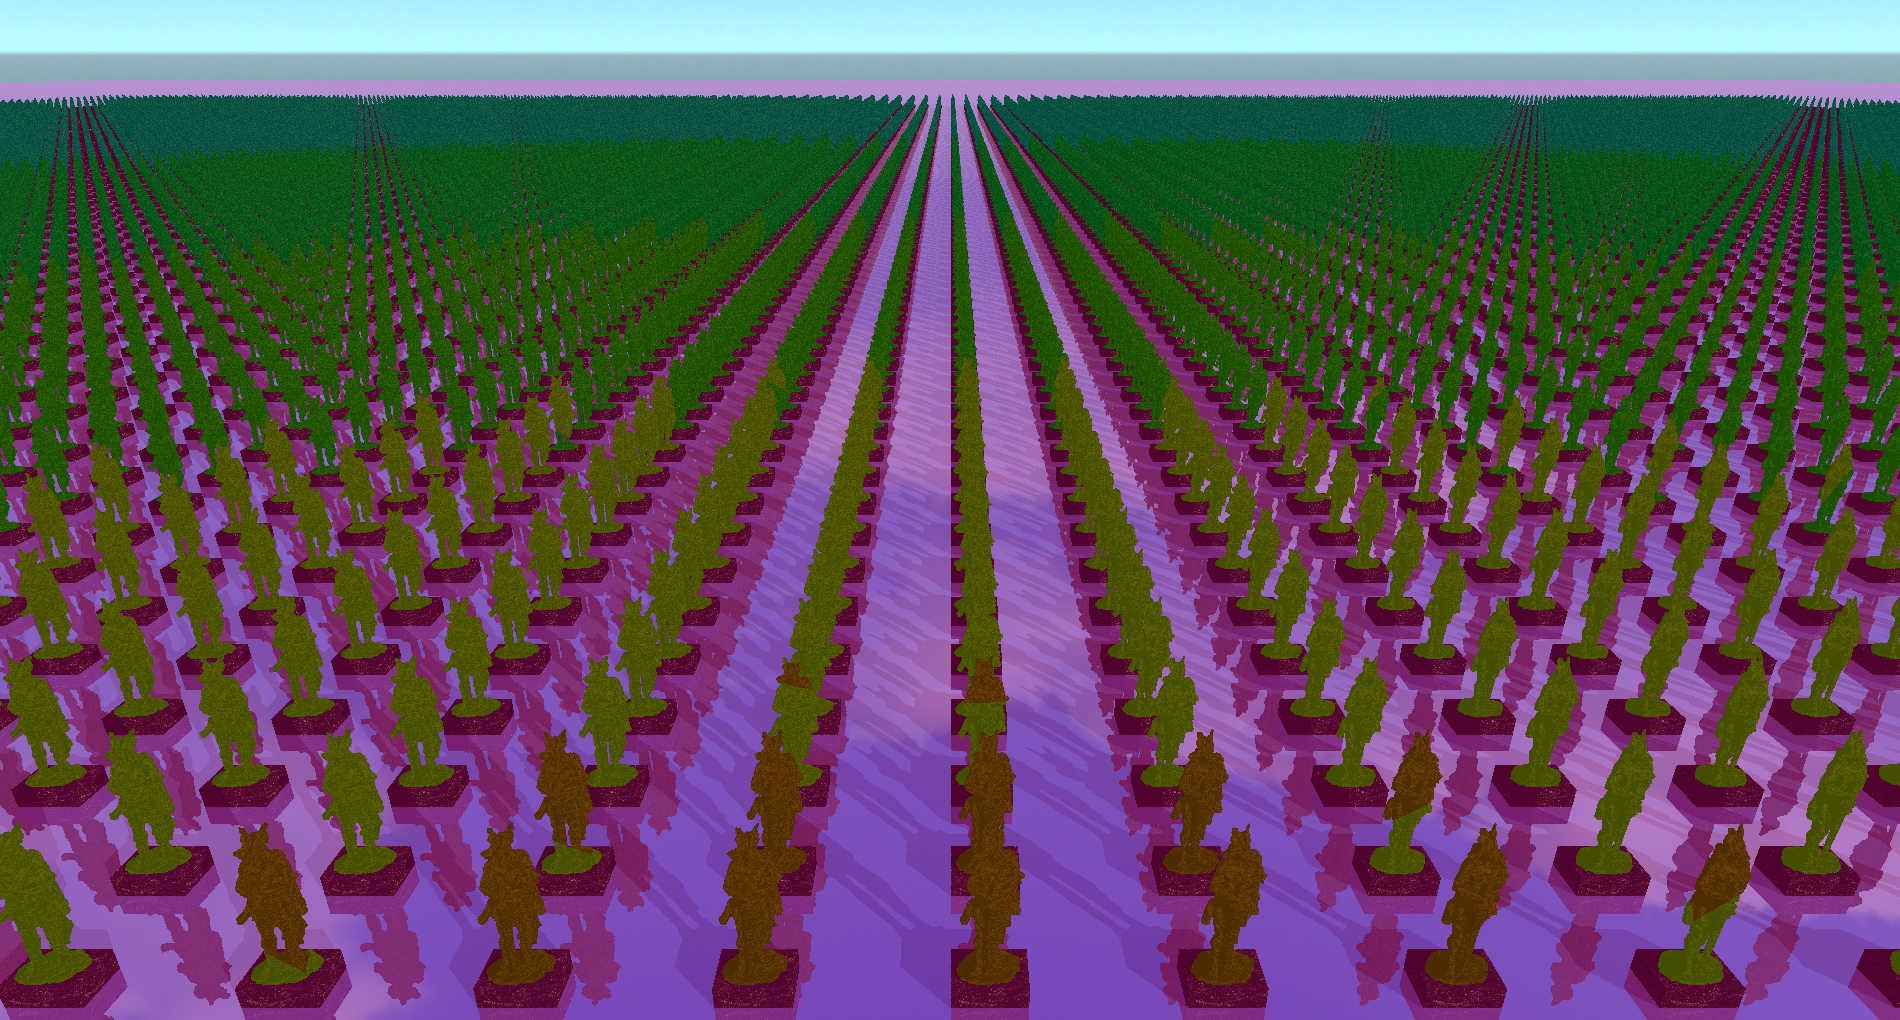
\includegraphics[width=.45\textwidth]{images/testing/LOD debug.PNG}}
\hfill
\caption{Displaying the LOD test scene. The chosen LOD is displayed left. The lowest LOD is green while more red indicates a high LOD.}
\label{fig:testLOD}
\end{figure}
To evaluate Level-of-Detail, we will be using an asset of a gallic statue (2.5M triangles) instanced multiple times around the scene. The LODs reduce the number of triangles by a factor of 4 for each level. The statue is instanced $128\times128$ times in x and z directions. We will be evaluating three different configurations. The total triangle count in the scene is (using the highest LOD) 41B. Each statue also has a footer and the scene uses a reflective and transparent ground.
\begin{enumerate}
    \item LOD6 - The instances reference an LOD-selector, which then decides on one of the six LODs. This scene uses a total 16385 instances. The 8 TLAS and 9 BLAS use a size of 234MB of VRAM.
    \item LOD1 - The LOD-selector always uses the highest LOD. The scene requires 3 TLAS and 4 BLAS which use a total of 178MB VRAM. The number of instances stays the same with 16385.
    \item LOD1-SL - The LOD-selector is removed and the scene is collapsed to a single level without changing the mesh. It requires 1 TLAS and 3 BLAS which total to a 188MB of VRAM used. The number of instances doubles to 32769 due to the footer being instanced as well.
\end{enumerate}
For all test scenes the total triangle count stays the same. (When using highest LOD). For LOD6 a total of 840k triangles are added for the LODs 1-5.
\newpage
\subsection{Results}
For testing, the camera is positioned in a way that lets the LOD impact performance well, which is high up so even far away statues are rendered. This is a beneficial test setup for the LOD. Profiling the application yields the following results:\\
\begin{center}
    \small{
\begin{tabular}{ |p{1.8cm}||p{0.7cm}|p{2.05cm}|p{1.8cm}|p{1.8cm}|p{2cm}|p{1.2cm}|  }
 \hline
 \multicolumn{7}{|c|}{LOD Results} \\
 \hline
 Test & FPS & Memory(MB) & L1-Hit(\%) & L2-Hit(\%) & Active pixel warps(\%) & RQ-Stall(\%)\\
 \hline
 LOD6   &   52  &   390 &   53,9    &   62,9    &   17,5    &   58,7\\
 \hline
 LOD1    &   42 &   296 &   48,2    &   53,0    &   17,6    &   61,0\\
 \hline
 LOD1-SL  &   47  &   308 &   38,4    &   40,2    &   18,2    &   72,5\\
 \hline
\end{tabular}
}
\end{center}
\begin{figure}
\hfill
\subfigure[LOD1-SL-Query Count]{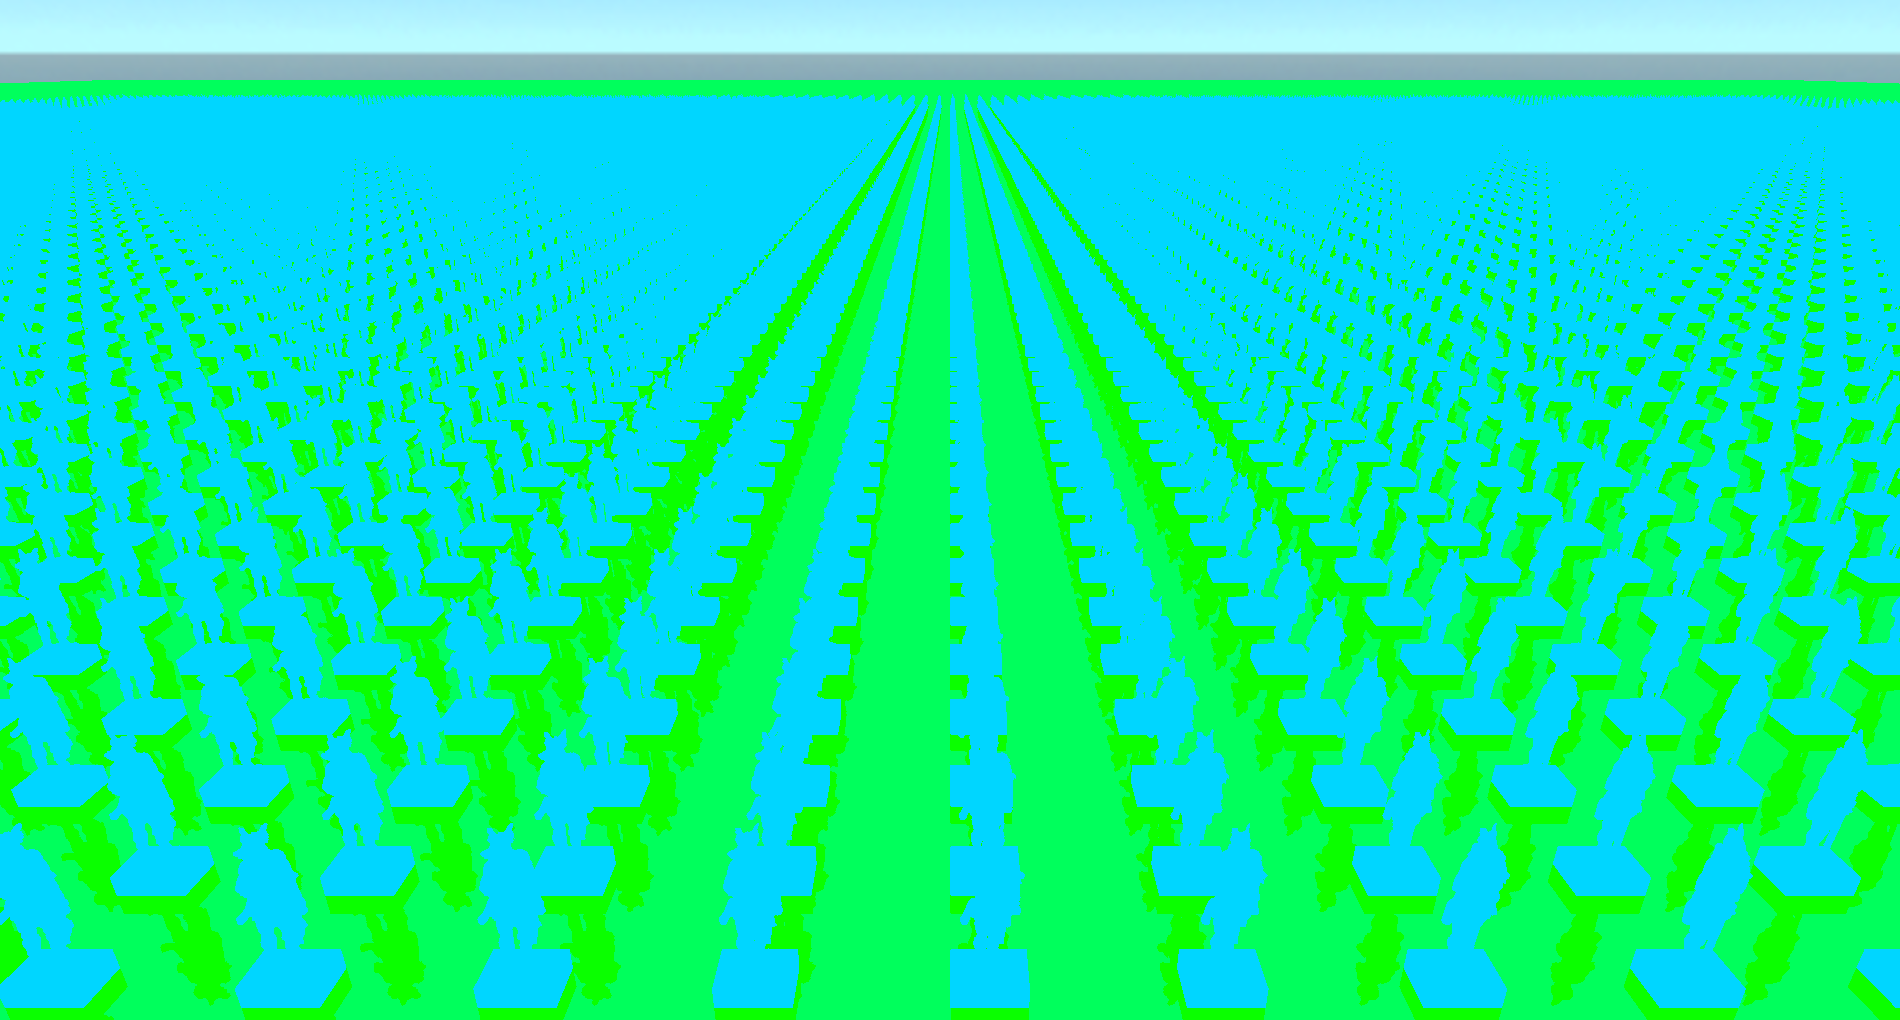
\includegraphics[width=.45\textwidth]{images/testing/LOD SL QueryCount.PNG}}
\hfill
\subfigure[LOD6-Query Count]{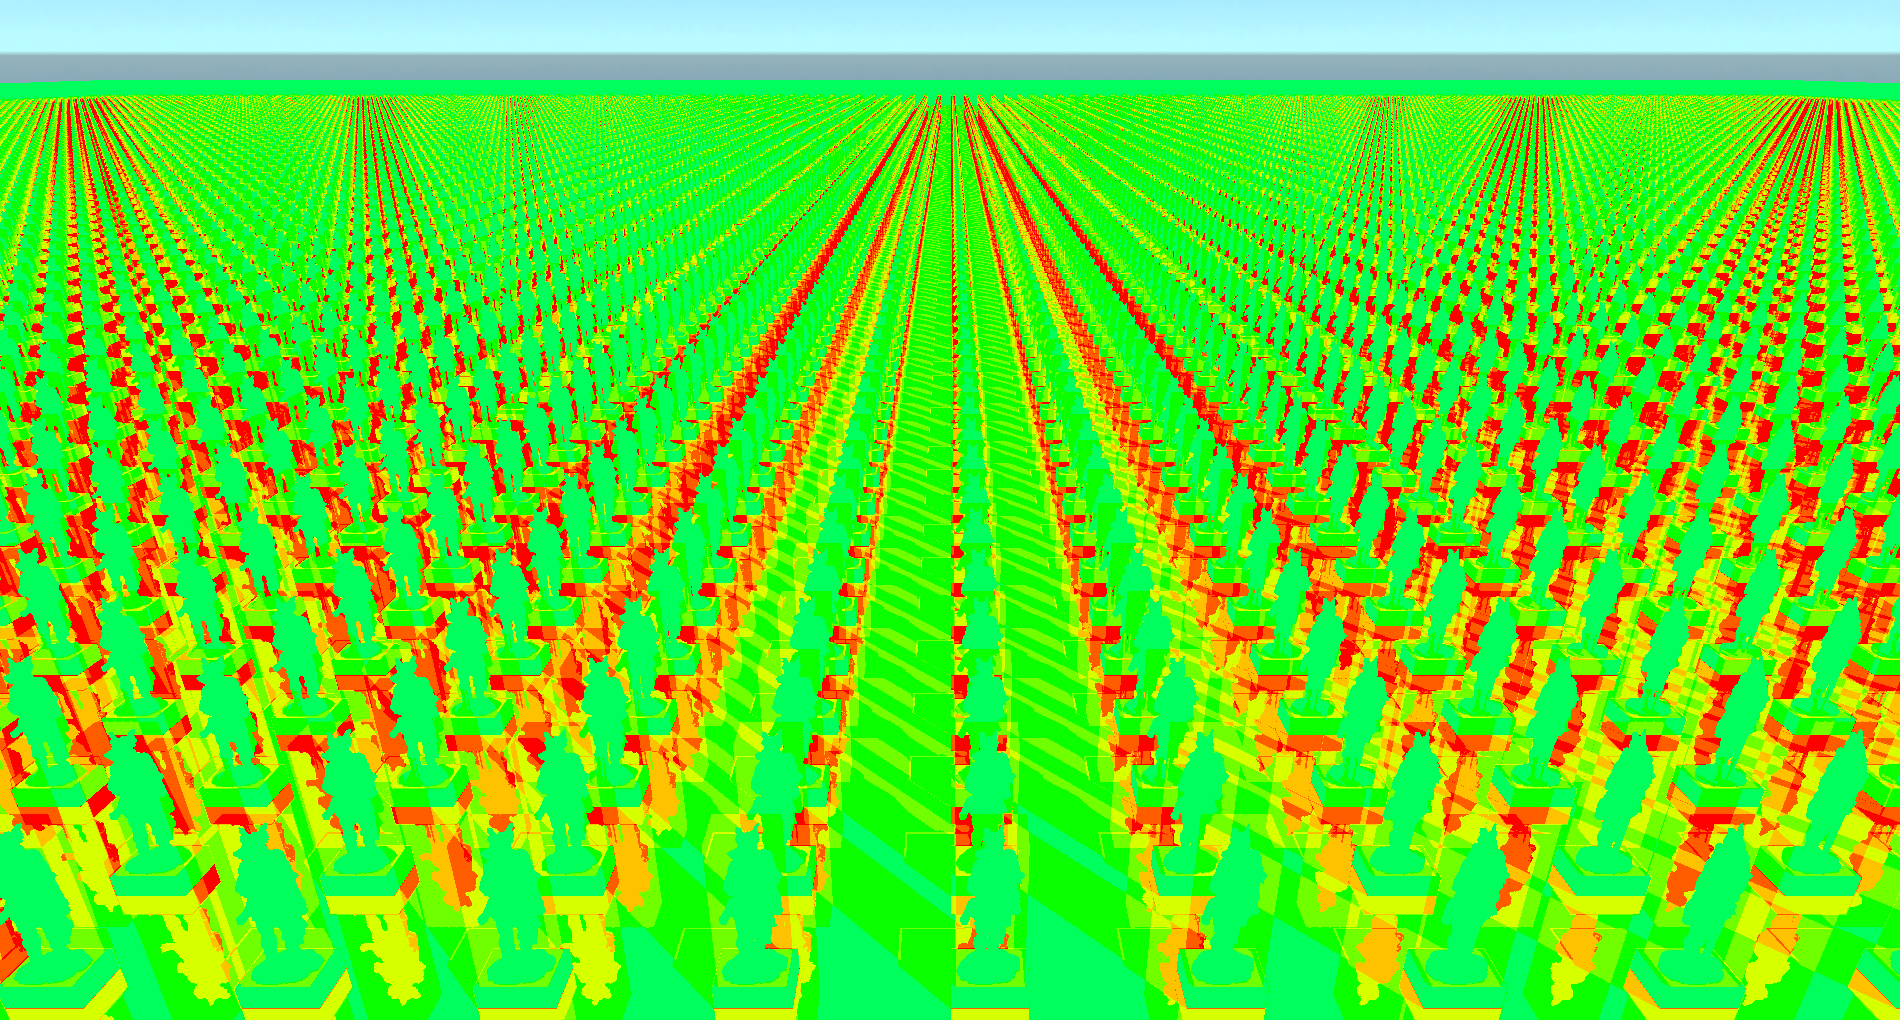
\includegraphics[width=.45\textwidth]{images/testing/LOD query count.PNG}}
\hfill
\caption{Number of ray queries (RQ). Red>15RQ, Blue$\approx$1RQ.}
\label{fig:LODRQCount}
\end{figure}
\subsection{Analysis}
In general the results show some promise for the usage of Level-of-Detail. I will now go into further detail regarding the various observed values.
\paragraph{FPS}
LOD increases the FPS by a small margin. The 42 FPS on LOD1 are also to be expected, since it is the same as LOD1-SL but with added traversal shader cost. However the perspective was deliberately chosen to display the effect LOD can have. When using a close-up view of the geometry where most of the screen is filled with a high level of detail, LOD1-SL will perform significantly better than LOD6.
\paragraph{Memory}
The increased memory for LOD6 is due to the added geometry. The increased memory for LOD1-SL is due to the added instances, since the traversal shader is not invoked and the footer and statue are no longer grouped together in a single instance.
\paragraph{Cache}
LOD offers benefits in cache efficiency due to the size of the traversed AS decreasing. This is due to the AS being smaller for far away objects. Cache rates of about 50\% are still bad, which is caused by the general size of the AS. As it uses 178MB in the smallest case and therefore requires a lot of memory swapping during traversal.
\paragraph{Pixel Warps and RQ-Stall}
The active pixel warps are limited by the amount of ray queries that can be fired on an SM in a given time period. This is caused by the high RQ-Stall. The increase form LOD6 to LOD1-SL is to be expected, given that in LOD6 some of the processing is shader code, as opposed to LOD1-SL where everything is calculated in a single ray query. This can be seen in \ref{fig:LODRQCount}. Nsight gives the stall reasons as primarily LSGB (long scoreboard) and MIO wait. Therefore, it is natural to assume that the shared use of the RT-Core between the different threads on the SM causes slowdowns. \cite{nvdiaCudaGuide}
\paragraph{Conclusion}
LOD can work in cases where there is a lot of geometry far away from the observer. The increase in memory is negligible unless the scene already uses a lot of memory. It also showed that cache can be improved by using LOD with traversal shaders. Though one has to keep in mind, that this test was designed to demonstrate usability not average performance. It is expected to see a decrease in performance when using LOD at low distances since then, the traversal cost reduction of LOD becomes negligible and the traversal shader cost increases.
\section{Multi-Level-Instancing}
\label{sec:INSTTEST}
Next up is evaluating the usage of Multi-Level-Instancing to reduce used VRAM as described in \ref{sec:instancing}.
\subsection{Setup}
\begin{figure}
\hfill
\subfigure[Rendered image]{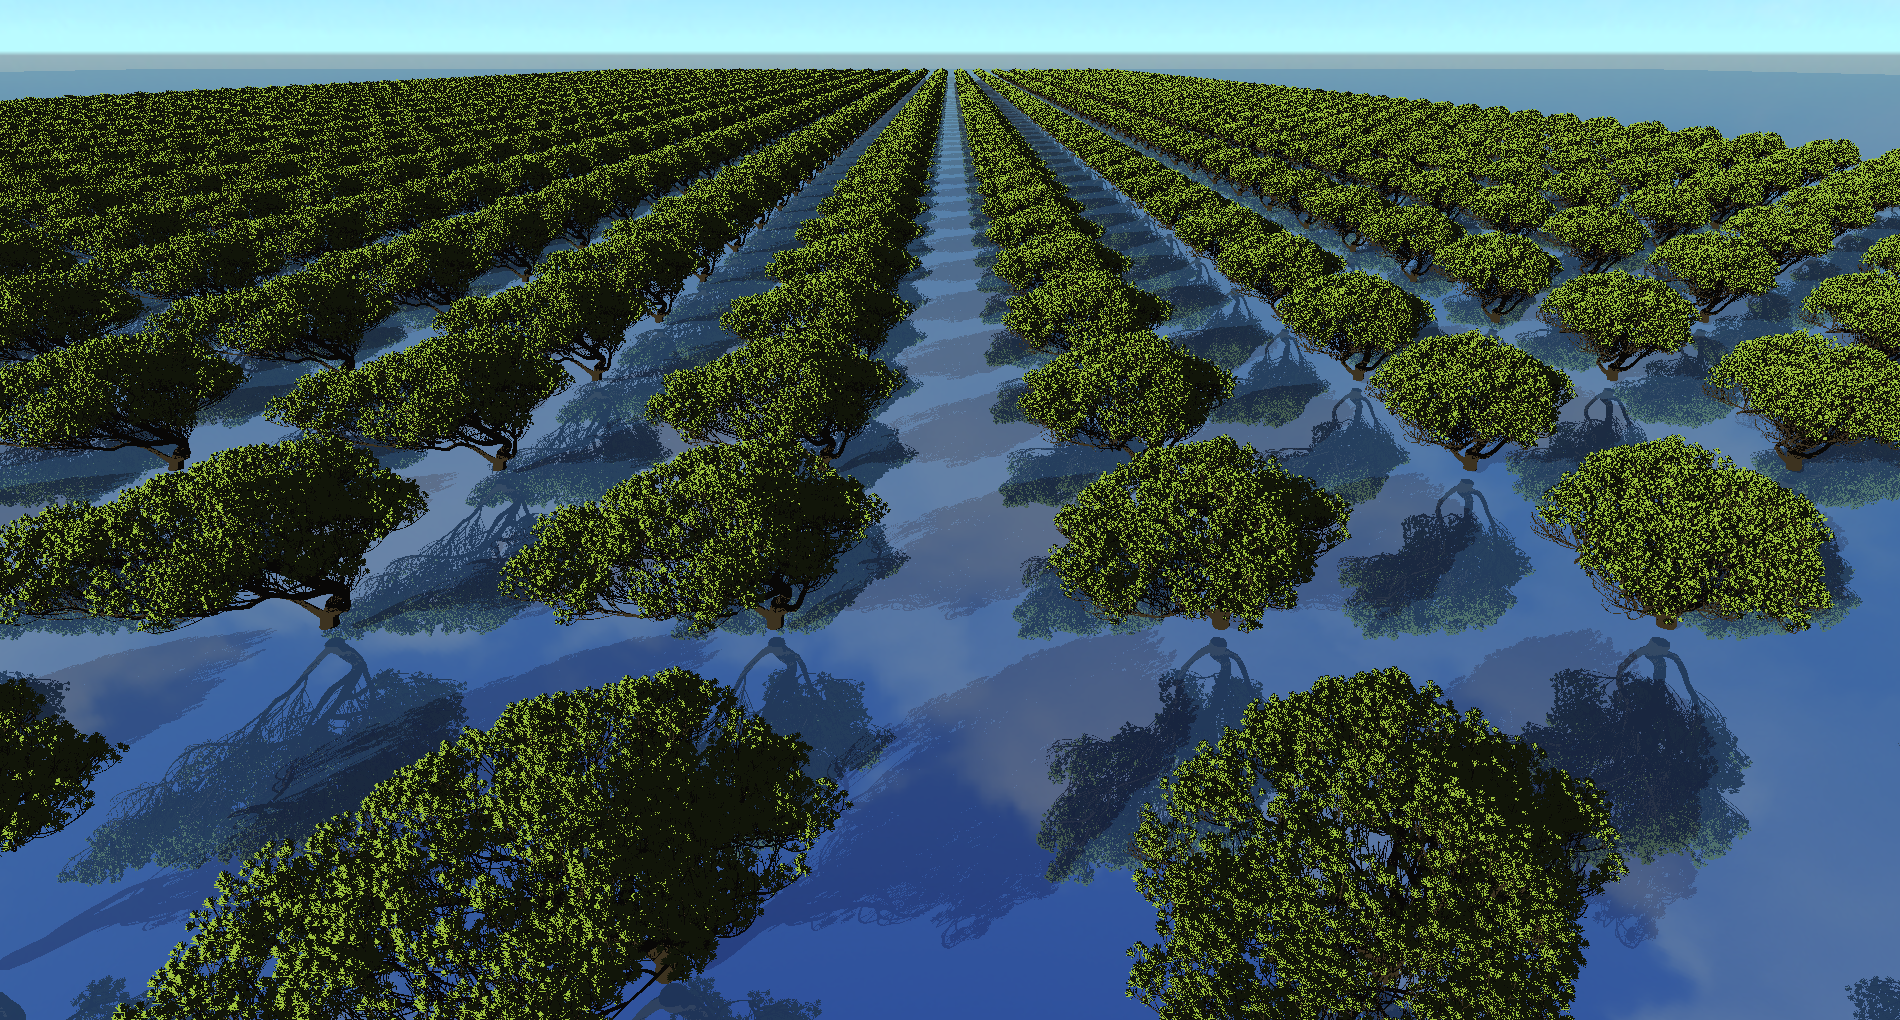
\includegraphics[width=.45\textwidth]{images/testing/Inst Render.PNG}}
\hfill
\subfigure[AABB Groups]{\includegraphics[width=.45\textwidth]{images/testing/Inst-ML-AABBs.PNG}}
\hfill
\caption{The Multi-Level-Instancing test scene (left) and the used AABB groups for the TLAS (right). Multiple trees are grouped together.}
\label{fig:MLRender}
\end{figure}
To evaluate the use of Multi-Level-Instancing we will use a tree from the Moana Island data set. The tree consists of one mesh that contains the trunk and branches with 1.9M triangles, its BLAS is 130MB in size. It then uses 8732 instanced leaves with a leaf mesh containing 864 triangles. The 8732 instances need a 5MB TLAS, the leaf geometry needs a <1MB BLAS. To assess the limits, we instance the tree as many times as possible, such that any further significant increase would put us over the TLAS instance limit $2^{24} \approx 16.7M$. This value is obtainable by using vkGetPhysicalDeviceProperties2 \cite{vulkanSpec}, it is device specific. We want to instance the scene in such a way that it barely fits onto a single level. This gives rise to the following calculation:
\begin{enumerate}
    \item Representing one tree with single-level instancing requires $8732+1$ (leaves+tree) instances.
    \item Number of tree instances possible: $2^{24}/8733 \approx 1921$.
    \item We want to use 3 levels when doing ML-Instancing. Therefore $\sqrt[3]{1921} \approx 12$
    \item A box instancing 4 times in x and 3 times in z direction achieves 12 instances
    \item The total instances on a single level:
    \[(3\cdot4)^3 \cdot 8733 + 1_{ground} = 15090625\]
    \item The total number of instances with multi level:
    \[(3\cdot4)\cdot3 + 8732 + 1_{ground} = 8769\]
    \item The total triangle count is therefore:
    \[(3\cdot4)^3 \cdot (8732 \cdot 864 + 1955190) + 2 = 16415374466 \approx 16B\]
\end{enumerate}
To clarify (6) an instance can refer to multiple children so the instance that refers to the list of leafs also refers to the mesh.\\
There still is some room, but if we use 3 levels of instanced trees and increase the instancing per level one further in any direction the number of instances exceeds device limitations. We now have the following tests:
\begin{itemize}
    \item SL-Max - Collapses the scene graph to a single level, it uses the mentioned 15M instances in a single TLAS, this TLAS has a size of 7132MB. It uses 3 BLAS (leaf, tree, ground). Total AS size: 7132MB
    \item ML-SL-EQ - This is the equivalent to SL-Max, but the tree remains uncollapsed. The number of instances is as in (6): 8769. It uses 5 TLAS and 7 BLAS. Total AS size is 135MB. 
    \item ML-Max - Increases instancing until it impossible for any SL scene to hold this many instances. The scene is instanced $32\times32$ 4 times. Through repeating the above calculation the triangle count is 10Q (quintillion). The instances on a single level would be 9q (quadrillion). It uses 6 TLAS and 8 BLAS which together use 138MB of memory.
\end{itemize}
\begin{figure}  
\hfill
\subfigure[SL-Query count]{\includegraphics[width=.45\textwidth]{images/testing/Inst SL-Query.PNG}}
\hfill
\subfigure[SL-EQ query count]{\includegraphics[width=.45\textwidth]{images/testing/Inst SL-EQ-Query.PNG}}
\hfill
\caption{The amount of ray queries by pixel. Red>45RQ, Blue$\approx$1RQ.}
\label{fig:MLQueryCount}
\end{figure}
\subsection{Results}
For this test, the observer is positioned in such a way that minimizes FPS. As the VRAM is static, it is beneficial to look at the performance impact. This is therefore a worst case test. Profiling yielded the following results:

\begin{center}
    \small{
\begin{tabular}{ |p{1.8cm}||p{0.7cm}|p{2.05cm}|p{1.8cm}|p{1.8cm}|p{2cm}|p{1.2cm}|  }
 \hline
 \multicolumn{7}{|c|}{LOD Results} \\
 \hline
 Test & FPS & Memory(MB) & L1-Hit rate(\%) & L2-Hit rate(\%) & Active pixel warps(\%) & RQ-Stall(\%)\\
 \hline
 SL-Max &   75  &   9096    &   67,6    &   56,5    &   17,9    &   85,0\\
 \hline
ML-SL-EQ    &   33  &   358 &   70,2    &   80,6    &   18,1    &   60,3\\
\hline
ML-Max  &   13  &   361  &  64,4    &   78,1    &   15,1    &   54,8\\
\hline
\end{tabular}
}
\end{center}

\subsection{Analysis}
As can be seen from the table, the usage of ML-instancing requires significantly more computation power. However, it can benefit memory massively. I will now go into further detail for the various results.
\paragraph{FPS}
The decrease in FPS is quite heavy. This is mostly due to the added traversal cost and massively increased number of ray queries, as can be seen in Figure \ref{fig:MLQueryCount}.
\paragraph{Memory}
The usage of ML-instancing can decrease memory usage by a huge margin, as can be seen from SL-Max to ML-SL-EQ. VRAM benefits especially well, as the AS are the main occupants of VRAM.
\paragraph{Cache}
Decreasing AS size results in improved cache efficiency. Which is definitely the case for the L2 caches for all tests. The drop in efficiency in L1 for ML-Max compared to SL-Max is difficult to explain. It could be that the number of memory accesses to the scene node and child index buffer increases heavily, which could justify these rates. But that is mostly speculation. Overall, ML-Instancing increases cache hit rates.
\paragraph{Pixel Warps and RQ-Stall}
These values follow the same pattern as in the LOD test. Using a single level increases RQ-Stall by quite a bit. However, this results in better performance due to the absence of traversal shader overhead. The pixel warps also follow the same pattern, as the RT core has to put in the most effort.
\paragraph{Conclusion}
Multi-Level-Instancing can decrease memory by huge margins. Though one has to pay attention that traversal cost does not become a problem. This is caused by non-occluding geometry, such as the used tree, as they tend to give many false positives for the instance intersections. This issue is normally solved with the query running as a whole on the RT core. This does not happen in this case which leads to increased cost and a rising number of ray queries. Additionally, the size of the traversal stack might become a problem if the number of intersected PIs grows too large.

\newpage
\begin{figure}
    \centering
    \includegraphics[width=.7\textwidth]{images/testing/Moana Render.PNG}
    \caption{Moana Island render @32FPS.}
    \label{fig:MoanaRender}
\end{figure}

\begin{figure}
    \centering
    \includegraphics[width=.7\textwidth]{images/testing/Moana ML-RE AABB.PNG}
    \caption{ML-RE contains multi-level instanced trees.}
    \label{fig:MoanaRenderAABBs}
\end{figure}
\section{Moana Island}
\label{sec:MOANATEST}
Moana Island represents the biggest and most realistic test. Here we will be using ML-instancing to show what the traversal shader can achieve. Creating LODs for the geometry was not feasible due to high AABB overlap, as it slowed down performance far too much by requiring more ray queries.
\subsection{Setup}
The setup uses the .pbrt format for the Moana Island scene. Moana island does not use classic UV-textures, instead it uses the Ptex texture format. Ptex is a per quad texture format. Supporting such a texture format would be quite cumbersome, so I opted to skip an implementation and instead use materials with fixed colors.\\
The parts of Moana we will use include 5M instances at lowest, with ML-instancing. A total of 22B triangles, 46M triangle primitives and 70M vertices. We will render Moana island with 4 different configurations.
\begin{itemize}
    \item SL-Max - Renders Moana Island with as many instances as possible while using only a single level. The count was approximated by lowering the amount of instances to a point where the VRAM would be sufficient enough to build and hold the AS. The number of instances in the TLAS is 15M with a size of 6583MB. This is not the maximum, but the build sizes do not allow for more, as the build scratch buffer would exceed VRAM size. It uses 1 TLAS and 236 BLAS. The total AS size is 9709MB. Build scratch buffer is about 1967MB for the TLAS.
    \item ML-UN - this is equivalent to SL-Max but uses Multi-Level-Instancing. The scene graph is only partially optimized and still contains a lot of overlapping AABBs. This configuration uses 19 TLAS and 254 BLAS. VRAM for the AS is 5925MB.
    \item ML-RE - the same as ML-UN but the scene graph is reduced to two levels of instancing. This configuration uses 5TLAS and 240 BLAS with a total AS VRAM usage of 5889MB. Figure \ref{fig:MoanaRenderAABBs} shows the AABBs used. The largest of which is the AABB for the entire scene. The small AABBs are trees that are multi-instanced. These are similar trees as the ones in the instancing test \ref{sec:INSTTEST}.
    \item ML-Max - tries to put ML-instancing to its limits by increasing the amount of instances until the AS can no longer be built. For this, the ASs are split such that the scratch buffer size is smaller, therefore resulting in 16 TLAS and 241 BLAS. Together these AS use a 10889MB of VRAM. The total triangle count increases by only 4M to 26M. This is due to all ML-instancing geometry already being included.
\end{itemize}
\subsection{Results}
For the results the observer will be placed in a spot that minimizes FPS for the SL test. From this position all other tests will be evaluated. Profiling the application gave these results:
\begin{center}
    \small{
\begin{tabular}{ |p{1.8cm}||p{0.7cm}|p{2.05cm}|p{1.8cm}|p{1.8cm}|p{2cm}|p{1.2cm}|  }
 \hline
 \multicolumn{7}{|c|}{LOD Results} \\
 \hline
 Test & FPS & Memory(MB) & L1-Hit rate(\%) & L2-Hit rate(\%) & Active pixel warps(\%) & RQ-Stall(\%)\\
 \hline
 SL-Max &   33  &   15479   &   64,4    &   43,9    &   18,4    &   89,5\\
 \hline
 ML-UN  &   21  &   10816   &   59,7    &   65,3    &   18,8    &   74,9\\
\hline
 ML-RE  &   32  &   10794   &   64,2    &   44,4    &   18,4    &   88,4\\
\hline
 ML-Max &   25  &   16900   &   57,5    &   67,0    &   18,8    &   ?\\
\hline
\end{tabular}
}
\end{center}
\newpage
\begin{figure}
\hfill
\subfigure[SL-Max Query count]{\includegraphics[width=.32\textwidth]{images/testing/Moana SL Max Query.PNG}}
\hfill
\subfigure[ML-UN Query count]{\includegraphics[width=.32\textwidth]{images/testing/Moana ML-UN Query.PNG}}
\hfill
\subfigure[ML-RE Query count]{\includegraphics[width=.32\textwidth]{images/testing/Moana ML-RE Query.PNG}}
\hfill
\caption{Query counts for various renders. Red>60, Blue$\approx$1RQ.}
\label{fig:MoanaQueryCount}
\end{figure}
\subsection{Analysis}
As the most realistic test Moana Island showed with ML-RE, that traversal shader can work if sufficient effort is put into optimizing the scene. I will now get into detail about each column.
\paragraph{FPS}
FPS is determined by a mix of the number of ray queries, traversal shader cost and AS size, so it is expected to see a decrease for ML-Max. Furthermore, scene optimization can have a significant performance impact. This can be seen with ML-UN and ML-RE, which are the same scene by the latter is optimized. Additionally, this is also indicated by the number of TLAS a scene uses, as they partially correspond to the maximum amount of traversal shader overhead that can occur. This can be seen in Figure \ref{fig:MoanaQueryCount}. The most surprising thing perhaps is that SL-Max and ML-RE perform equally as good. Indicating that if using ML-Instancing with a low AABB overlap has no significant impact on performance but reduces memory by a lot.
\paragraph{Memory}
ML-UN and ML-RE as expected decrease memory usage significantly, while the latter keeping up in FPS. This is a good use-case for real-world, real-time applications. Though it has to be done in moderation as the \ref{sec:INSTTEST} showed. This test also showed that the build scratch size can decrease the possible number of instances as well, due to it easily requiring 1.5GB of VRAM for the build. This can be solved by splitting large TLAS into smaller as with the isBeach split in \ref{sec:OptInstanceOverlap}.
\paragraph{Cache}
As with the previous tests it shows that smaller AS lead to better cache hit rates, especially for the L2 cache. However, these values are difficult to explain. SL-Max and ML-RE behave similarly, as ML-RE has a very large TLAS for the entire scene just like SL-Max. The high L1 hit rate    s for those two could be explained by the usage of their BLAS, since in both cases, the BLAS are similarly small. This would also explain ML-UN and ML-Max as they all use the same BLASs. The improved efficiency for ML-UN and ML-Max is also to be expected, this is due to the root TLAS for the entire scene being split into multiple parts, which leads to the improved cache hit rate like in the ML-Instancing test \ref{sec:INSTTEST}.
\paragraph{Pixel Warps and RQ-Stall}
As before the Pixel warps are again limited by the availability of the RT-Core. SL-Max and ML-RE also spend most of their time executing ray queries, since both graphs are optimized to do so. ML-UN uses the traversal shader significantly more, which results in the RQ-Stall being lower than for the other two. For ML-Max no RQ-Stall could be measured due to the additional amount of VRAM Nvidia Nsight uses. This led to the scene not being able to allocate their buffers.
\paragraph{Conclusion}
This test shows the real world application for traversal shaders, and the results are promising. With enough consideration traversal shaders can decrease AS size by $\approx$40\% and still keep the framerate next to equal. They also improve cache efficiency in most cases, but suffer from the limitation of the RT-Core.

\section{Discussion}
While there are many things to talk about, the tests showed a couple of things which need to be considered when using traversal shaders.
\begin{itemize}
    \item LOD - Level of detail can work, if applied correctly. However, it is necessary to figure out if LOD is actually required for an object. Examples would be mountains that are really far away from the observer. If the observer comes close, they offer much more detailed geometry. LOD is unnecessary for large counts of small objects, as it increases traversal shader cost and leads to overlapping AABBs. Therefore LOD is the most beneficial for large, high-resolution geometry. Due to the logarithmic traversal times an AS provides \ref{sec:BVH}, a decrease in geometry by a factor only results in a constant decrease in query time, which is the primary reason why LOD offers only a small benefit.
    \item Multi-level - The traversal shader with Multi-Level-Instancing suffers a lot from non occluding geometry, especially with trees like in the instancing test \ref{sec:INSTTEST}. However when it comes to real applications it can decrease memory usage by quite a lot and still keep up a good frame rate. Here, moderation is the most important aspect. ML-Instancing should only be used if the geometry would be much too large for a normal BLAS. Additionally, AABB overlap plays an important role. Therefore ML-Instancing is most promising in enclosed spaces that are separated from each other by geometry like walls or mountains that do not use multi-level instancing or are at least on level that is lower than the instanced geometry.
    \item Ray queries - The hardware for raytracing is good beyond any doubt. However, it has limitations, as every single test ran showed more than 60\% of shader time is spent executing the ray query. But there are ways to make ray queries more efficient, which I talked about before \ref{sec:OptQuerySpeed}. The main problem being overlapping AABBs as well as AABBs that are only intersected but do not return a hit. Holes in geometry for example.
\end{itemize}

Memory might be the biggest reason why anyone would be using traversal shading, as framerate almost always drops when using traversal. The results show that with the right scene layout and sufficient scene graph optimization, traversal can save vast amounts of memory while only impacting performance slightly. The bottleneck is latency between memory, shader, and RT-core. All of these can be improved with an integrated pipeline and enhanced raytracing capabilities. It is definitely possible for such improvements to arrive in the near future, as GPU vendors keep improving on their real-time realism with raytracing.

\chapter{Summary}
In this chapter, I will summarize what we have learned and how to go from this point on.
\section{Results}
This thesis showed that traversal shaders do, in fact, work in a couple of scenarios. As the Moana Island test \ref{sec:MOANATEST} showed, they are able to reduce memory usage by 40\% and still keep the frame rate next to equal. However, in some cases, they are not as efficient. These are the cases where traversal continues through multiple AS, but the closest hit comes very late. In those cases they can still reduce memory by over 90\% but also reduce framerate by 50\% or more.\\
With the high RQ-Stall, the tests also show a limit for raytracing on the current GPUs. This can be attributed to the availability of only one RT-Core as well as the interaction between shader and RT-Core consuming too much time. Another issue are the partially very bad cache-hit rates. The traversal shader shows to improve them a little, but there is much room for improvement. Low cache hit rates mostly occur due to very large AS sizes. Traversal shaders can help with this.\\
Traversal speed improves massively though the presence of occluding objects like mountains or walls. It suffers from partially non-occluding geometry. This problem is native to AS in general, but traversal shaders make it worse due to traversal being interrupted by the instance shader.\\
Considering distribution and overlap, the performance of traversal shaders depends highly on the density of PIs in an AS in local areas. Applications implementing traversal shaders should make sure that any traversal though an AS does not intersect more than predefined number of PIs from any angle. This threshold number can be determined experimentally, but it should give a good indication for performance. For (Moana Island \ref{sec:MOANATEST}) the maximum PIs intersected was about 5 and they did not overlap.
\section{Leftover issues}
The most pressing issue is latency between RT-Core, shader, and VRAM. Large scene and AS sizes directly correspond to a high traversal cost. Even when not using traversal shaders at all. Therefore, AS compaction can deal with memory sizes. This would also result in an improved cache-efficiency and therefore faster traversal. Another way to deal with low cache efficiency is grouping rays of neighboring pixels into a thread group that is executed on the same SM.\\
Traversal speed is largely determined by the convergence of the t-Value. So, it is necessary to traverse AABBs with low t-Near values first before higher ones. However, there is no guarantee for this, so it might be worthwhile to look into techniques to optimize the traversal stack, by sorting it a bit.\\
Another thing worth trying might be dedicated code implementation for various types of Nodes. For example, if a node only has geometry and no PIs, then it could be flagged as geometry-only. Then a traversal loop could be used that only implements this functionality, therefore saving a few case switches while the loop is running.
\section{Best usage}
\label{sec:BestUsage}
Traversal shaders show the most promising results on systems with sufficient computation power. Scenes that use multi-level instancing benefit the most, especially if the geometry is in an enclosed space. Best candidates are trees, houses, and other reoccurring groups. Scenes should be optimized with traversal in mind to achieve the most improvement. If that is the case, traversal shader can improve performance slightly (with LOD) and memory greatly (with ML-Instancing). Moderation in using traversal and thorough consideration is key.
A good use-case would be instanced rooms in a house with the following pattern:
\begin{enumerate}
    \item LVL0 - House - TLAS - contains BLAS references for house walls and one BLAS that contains a PI for each room
    \item LVL1 - House wall - BLAS - contains triangle geometry
    \item LVL2 - Room - TLAS - with BLAS references for walls and BLAS references for geometry inside the room
    \item LVL3 - Room wall - BLAS - contains triangle geometry
    \item LVL3 - Room geometry - contains either direct triangle geometry or a PI to a multi-instanced object
    \item LVL4 - PI - multi-instanced objects like flowers
    \item LVL5+ - geometry for multi-instanced objects, possible deeper tree for example for a doll-house with instanced rooms
\end{enumerate}
To avoid the performance trap \ref{sec:OptStackSize} it is necessary for the TLAS to represent the collection of instances and not an instance itself. The instances should be represented by BLAS-references in a TLAS. This becomes extremely important when the instances are close or even overlapping! The presence of walls basically guarantees that no more than one PI for a room is traversed, unless the observer stands before an open door.
\section{Outlook}
A full raytracing pipeline can benefit from traversal shaders. However, for now the better practice remains the usage of a visibility and shading pass for a minimal amount of ray queries. The traversal shader can be used in a couple of cases. Overhead only is added if there are actually PIs in an AS, otherwise it behaves like any closest hit RQ. It is definitely worth considering integrating a version of this if an application uses a group of instances multiple times. Furthermore, modifying traversal can be quite handy in other cases. One such example would be the implementation of a portal or other light path manipulating objects.\\
The next approach tries to minimize memory even further by using a lazy build as proposed by Won-Jong et al. \cite{traversalLazyBuild}. It uses the separation of instances inside AS to construct them on demand. For example, an application could have one TLAS for the entire world and then use a lazily build the AS for the specific parts of the scene depending on where the observer is currently positioned. This would result in saving memory by not building the ASs for geometry that has no impact on the rendered image. This is useful because currently the AS are much larger than the geometry they are based upon, even when using compaction techniques. The house-example for the best usage \ref{sec:BestUsage} is one such case where a lazy build would work great.\\
Another promising example would be moving instances. If the range of movement for an object is known, then it is possible to hull the object inside an AABB and let traversal do the intersection using a separate query. This works because the traversal shader can transform the ray in any way it wants, so it can also offset the ray in such a way that it represents the movement of the object. This completely removes the requirement to rebuild the AS for such objects. It would require passing the required values by updating the node in the node buffer and adjusting the traversal shader accordingly. There is a small drawback here though, an application implementing this must  pay attention that AABBs do not overlap as much. Another way this could be applicable would be to reduce the requirement to rebuild an AS. The AABB could be multiple times the size of the object, resulting in the AS being less often required to be updated when the object is moving, even if the range of movement is not known.\\
The shader that was developed during this thesis is definitely not optimal, so there is room for improvement here too.

\section{Further reading}
Further reading on raytracing with Vulkan \cite{vulkanNvidia}, \cite{vulkanRayTracing}. For basic knowledge of Vulkan see the Vulkan-Tutorial \cite{vulkanTutorial} as well as the Vulkan-Specification can help \cite{vulkanSpec}. For basics in computer graphics my main source of knowledge was the CG lecture@KIT, but also the open book \cite{pbrBook} and Scratchapixel \cite{scrathAPixel} were great sources.

\section{Acknowledgements and thanks}
This might give a good outlook into the future and may prepare for any future developments. My thanks go out to all the great sources available as well as the code which mine is based or took inspiration from, that being Christoph Peters \cite{momentsingraphics} and his toy renderer, the Vulkan tutorial \cite{vulkanTutorial}and the well maintained Vulkan Spec \cite{vulkanSpec}. Thanks also to the KIT, especially the Computer Graphics lecture by Prof. Carsten Dachsbacher and my thesis supervisor Killian Herveau.  Thanks go also out to the open-sources that were used in this thesis, that being the Vulkan-Lunar-SDK, GLFW, Dear ImGui, vcglib and the Moana Island scene \cite{moanaIsland}. That is all.

\begin{center}
    Thank you for reading.
\end{center}